% ---
% Capitulo Análises
% ---
\chapter{Análises Realizadas}\label{chap:analises}

\section{Estatísticas Descritivas}\label{sec:bd-estat-descr}

A seguir serão apresentadas algumas estatísticas descritivas das variáveis, bem como outras observações julgadas pertinentes.

A variável \textbf{ANO}, de natureza qualitativa, não possui ``NA'' e conta com quatro valores únicos, cujas frequências absolutas são apresentadas na Tabela \ref{tab:estat-ano}. Esta variável não era original dos bancos de dados e foi inserida para poder gerar \textit{dummies} de marcação da \textit{cross-section} observada para análises de caráter longitudinal.

\begin{table}[htb]
    \IBGEtab{%\renewcommand{\arraystretch}{1.5}%%\ABNTEXfontereduzida%
        \renewcommand{\arraystretch}{1.5}
        \caption{Estatísticas da variável ``ANO''}
        \label{tab:estat-ano}
    }{%
        \begin{tabular}{P{3.00cm} P{4.0cm}}
            \toprule
               \headerTabCenterCell{Categoria} &
               \headerCell{Frequência Absoluta} \\
            \midrule \midrule
                1 - 1977 & 229.046\\
            \midrule
                2 - 1987 & 223.926\\
            \midrule
                3 - 1997 & 199.640\\
            \midrule
            4 - 2007 & 196.698\\
            \bottomrule
        \end{tabular}
    }

\end{table}
% Estatísticas para todos os registros da base

A variável \textbf{CD_ENTRE}, \textit{dummy}, não possui ``NA'' e conta com dois valores únicos (0 e 1) em que o 1 indica se houve viagem (83\%) e 0, se não houve viagem (17\%) . Sua frequência absoluta, segundo o ano e sexo é apresentada na Tabela \ref{tab:estat-cd-entre}.

\begin{table}[htb]
\centering
   \IBGEtab{%\renewcommand{\arraystretch}{1.5}%%\ABNTEXfontereduzida%
        \renewcommand{\arraystretch}{1.5}
        \caption{Estatísticas da variável ``CD_ENTRE''}
        \label{tab:estat-cd-entre}
    }{%

    \begin{tabular}{cccccc}
        \toprule
        \textbf{ANO} & \textbf{1977} & \textbf{1987} & \textbf{1997} & \textbf{2007} & \textbf{Total}\\ \midrule \midrule
        \textbf{CD\_ENTRE=0} & 41.514  & 40.808  & 36.106  & 27.033  & 145.461 \\ \hline
        \textbf{CD\_ENTRE=1} & 187.532 & 183.118 & 163.534 & 169.665 & 704.849 \\ \bottomrule
        \end{tabular}
    }

\end{table}
% Estatísticas para todos os registros da base

A variável \textbf{DIA_SEM}, de natureza qualitativa, conta com cinco valores únicos, cujas frequências absolutas são apresentada na Tabela \ref{tab:estat-dia-sem}.
Ela possui 296.893 registros ``NA'', sendo 229.046 de 1977, ano em que esta variável não foi levantada. Os demais \textit{missing values} foram adotados para o caso em que os valores eram originalmente iguais a 0, dividindo-se entre os anos de 1987 e 2007 e indicando observações relativas a não-viagens. Nas transformações efetuadas na preparação da base de dados, em 1987, foram feitas duas correções porque pressupôs-se erro de preenchimento: (i) 187 casos com registro 1 (valor que não consta nos layouts oficiais) que foram transformados para 2 (segunda-feira); e (ii) 170 casos de registro 7 (valor que não consta nos layouts oficiais) que foram transformados para 6 (sexta-feira).
 Vale observar que a sexta-feira (DIA_SEM=6) é superrepresentado devido à metodologia de coleta utilizada: na pesquisa, domiciliar, pregunta-se ao(à) respondente sobre as viagens que fizera no dia anterior e sábado é o dia em que mais se encontram as pessoas em casa, assim, há mais respostas sobre a sexta-feira do que sobre os demais dias da semana.

\begin{table}[htb]
    \IBGEtab{%\renewcommand{\arraystretch}{1.5}%%\ABNTEXfontereduzida%
        \renewcommand{\arraystretch}{1.5}
        \caption{Estatísticas da variável ``DIA_SEM''}
        \label{tab:estat-dia-sem}
    }{%

    \begin{tabular}{cccccc}
        \toprule
        \textbf{ANO} & \textbf{1977} & \textbf{1987} & \textbf{1997} & \textbf{2007} & \textbf{Total}\\ \midrule \midrule
        \textbf{DIA_SEM=2} & 0 & 27.771 & 32.956 & 25.129 & 85.856\\ \hline
        \textbf{DIA_SEM=3} & 0 & 34.089 & 36.817 & 23.764 & 94.670\\ \hline
        \textbf{DIA_SEM=4} & 0 & 35.275 & 37.695 & 27.242 & 100.212\\ \hline
        \textbf{DIA_SEM=5} & 0 & 33.003 & 32.924 & 28.010 & 99.937\\ \hline
        \textbf{DIA_SEM=6} & 0 & 52.980 & 59.248 & 65.514 & 177.742\\ \bottomrule
        \end{tabular}
    }

\end{table}
% Estatísticas para todos os registros da base

As variáveis \textbf{UCOD} (domicílio, escola, trabalhos, origem e destino), qualitativas, estabelecem correspondência com as zonas conforme Anexo \ref{chap:anexo_ucod}.

As \textbf{ZONAS} e \textbf{SUBZONAS} (domicílio, escola, trabalhos, origem e destino), qualitativas, de cada ano podem ser observadas no Anexo \ref{chap:anexo_mapas_zonas}. Não foi disponibilizado o mapa com as subzonas de 1977 e, em 2007, não existem subzonas.

As \textbf{coordenadas X e Y} (domicílio, escola, trabalhos, origem e destino), variáveis métricas, foram extraídas diretamente dos mapas pelo uso do software QGIS \footnote{``O QGIS é um Sistema de Informação Geográfica (SIG) de Código Aberto licenciado segundo a Licença Pública Geral GNU.'' Fonte: \url{http://www.qgis.org/pt_BR/site/about/index.html} Acesso em 26 de dezembro de 2015}. Em 1977, elas foram determinadas a partir dos centroides das zonas. Em 1987 e 1997, elas foram determinadas a partir dos centroides das subzonas. Já em 2007, o levantamento contou com a tecnologia GPS\footnote{GPS significa \textit{Global Positioning System} e é um sistema de posicionamento que permite localização em qualquer ponto da Terra desde que o receptor móvel esteja no campo de visão de quatro satélites GPS. Até meados dos anos 2000, a utilização do GPS para uso civil ainda tinha pouca precisão.} e o banco de dados já continha as coordenadas.

As variáveis \textbf{F_DOM}, \textbf{F_FAM} e \textbf{F_PESS} são \textit{dummies} que identificam o primeiro registro do domicílio, família e pessoa, respectivamente. Não contam com ``NA'' e têm suas frequências absolutas apresentadas pelas Tabelas \ref{tab:estat-f-dom}, \ref{tab:estat-f-fam} e \ref{tab:estat-f-pess}. Vale observar que os valores correspondentes a F_DOM=1, F_FAM=1 e F_PESS=1 significam exatamente os tais de domicílios, famílias e pessoas entrevistados em cada um dos anos.

\begin{table}[htb]
\centering
   \IBGEtab{%\renewcommand{\arraystretch}{1.5}%%\ABNTEXfontereduzida%
        \renewcommand{\arraystretch}{1.5}
        \caption{Estatísticas da variável ``F_DOM''}
        \label{tab:estat-f-dom}
    }{%

    \begin{tabular}{cccccc}
        \toprule
        \textbf{ANO} & \textbf{1977} & \textbf{1987} & \textbf{1997} & \textbf{2007} & \textbf{Total}\\ \midrule \midrule
        \textbf{F\_DOM=0} & 204.433 & 197.856 & 175.799 & 166.741 & 744.829 \\ \hline
        \textbf{F\_DOM=1} &  24.613 &  26.070 &  23.841 &  29.957 & 104.481 \\ \bottomrule
        \end{tabular}
    }

\end{table}
% Estatísticas para todos os registros da base

\begin{table}[htb]
\centering
   \IBGEtab{%\renewcommand{\arraystretch}{1.5}%%\ABNTEXfontereduzida%
        \renewcommand{\arraystretch}{1.5}
        \caption{Estatísticas da variável ``F_FAM''}
        \label{tab:estat-f-fam}
    }{%

    \begin{tabular}{cccccc}
        \toprule
        \textbf{ANO} & \textbf{1977} & \textbf{1987} & \textbf{1997} & \textbf{2007} & \textbf{Total}\\ \midrule \midrule
        \textbf{F\_FAM=0} & 202.889 & 195.709 & 172.795 & 165.843 & 737.236 \\ \hline
        \textbf{F\_FAM=1} &  26.157 &  28.217 &  26.845 &  30.855 & 112.074 \\ \bottomrule
        \end{tabular}
    }

\end{table}
% Estatísticas para todos os registros da base

\begin{table}[htb]
\centering
   \IBGEtab{%\renewcommand{\arraystretch}{1.5}%%\ABNTEXfontereduzida%
        \renewcommand{\arraystretch}{1.5}
        \caption{Estatísticas da variável ``F_PESS''}
        \label{tab:estat-f-pess}
    }{%

    \begin{tabular}{cccccc}
        \toprule
        \textbf{F\_PESS=0} & \multicolumn{4}{c}{\textbf{ANO}} & \multirow{2}{*}{\textbf{Total}} \\ \cline{1-5}
        \textbf{SEXO}      &  \textbf{1977} & \textbf{1987} & \textbf{1997} & \textbf{2007} & \multicolumn{1}{c}{} \\ \midrule \midrule
        \textbf{Masculino} &  72.040   &  62.264   &  52.146   &  51.732   & 238.182 \\ \hline
        \textbf{Feminino}  &  48.978   &  50.849   &  48.714   &  53.561   & 202.102 \\ \hline
        \textbf{Total}     & 121.018   & 113.113   & 100.860   & 105.293   & 440.284 \\\bottomrule

        \textbf{F\_PESS=1} & \multicolumn{4}{c}{\textbf{ANO}} &\multirow{2}{*}{\textbf{Total}} \\ \cline{1-5}
        \textbf{SEXO}      & \textbf{1977} & \textbf{1987} & \textbf{1997} & \textbf{2007} & \multicolumn{1}{c}{} \\ \midrule \midrule
        \textbf{Masculino} &  52.162   &  53.176   &  47.326   &  42.289   & 194.953 \\ \hline
        \textbf{Feminino}  &  55.866   &  57.637   &  51.454   &  49.116   & 214.073 \\ \hline
        \textbf{Total}     & 108.028   & 110.813   &  98.780   &  91.405   & 409.026 \\\bottomrule
        \end{tabular}
    }

\end{table}
% Estatísticas para todos os registros da base

As variáveis \textbf{FE_DOM}, \textbf{FE_FAM} e \textbf{FE_PESS}, variáveis métricas, são fatores de expansão (pesos) de domicílio, família e pessoa, respectivamente, já fornecidos pelas bases de dados e que não sofreram transformação alguma.

Os fatores de expansão da família e da pessoa têm intervalos praticamente iguais aos do domicílio (ver Tabela \ref{tab:estat-fe-dom}), sendo que as médias, medianas e intervalos inter-quartis se alteram, pouco, dentro do mesmo ano.
O Gráfico \ref{graf:freq-abs-fe-dom} apresenta as distribuições por ano da variável FE_DOM, cujo máximo valor da abscissa ficou em 550 pois o maior valor do intervalo inter quartil foi 535,5 em 2007. As variáveis FE_FAM e FE_PESS possuem distribuições bastante semelhantes a esta.


\begin{table}[htb]
\centering
   \IBGEtab{%\renewcommand{\arraystretch}{1.5}%%\ABNTEXfontereduzida%
        \renewcommand{\arraystretch}{1.5}
        \caption{Estatísticas da variável ``FE_DOM''}
        \label{tab:estat-fe-dom}
    }{%

    \begin{tabular}{cccccc}
        \toprule
        \textbf{ANO} & \textbf{Mínimo} & \textbf{1º Quartil} & \textbf{Mediana} & \textbf{3º Quartil} & \textbf{Máximo}  \\ \midrule \midrule
        \textbf{1977}  & 0,50 & 25,75 &  72,09 & 139,25 & 1562,75 \\ \hline
        \textbf{1987}  & 1,02 & 78,32 & 110,49 & 150,89 & 2210,00 \\ \hline
        \textbf{1997}  & 1.00 & 51,41 & 117,14 & 213,09 & 2548,63 \\ \hline
        \textbf{2007}  & 2,55 & 40,92 &  87,42 & 234,90 & 2256,41 \\ \hline
        \textbf{Geral} & 0,50 & 48,67 &  99,20 & 174,06 & 2548,63 \\ \bottomrule
        \textbf{ANO} & \textbf{Média} & \textbf{Desvio Padrão} & \textbf{Assimetria} & \textbf{Curtose} & \textbf{Nº de ``NA''}  \\ \midrule \midrule
        \textbf{1977}  &  94,92 &  92,42 & 2,63 & 18,78 & 0 \\ \hline
        \textbf{1987}  & 127,53 &  90,95 & 5,02 & 54,44 & 0 \\ \hline
        \textbf{1997}  & 178,75 & 209,77 & 3,51 & 20,44 & 0 \\ \hline
        \textbf{2007}  & 183,82 & 228,96 & 2,69 & 10,66 & 0 \\ \hline
        \textbf{Geral} & 147,67 & 174,64 & 3,79 & 23,63 & 0 \\ \bottomrule
        \end{tabular}
    }

\end{table}

\begin{grafico}[htb]%
    \caption{\label{graf:freq-abs-fe-dom}Distribuição da variável ``FE_DOM'', por ano}%
    \begin{center}%
        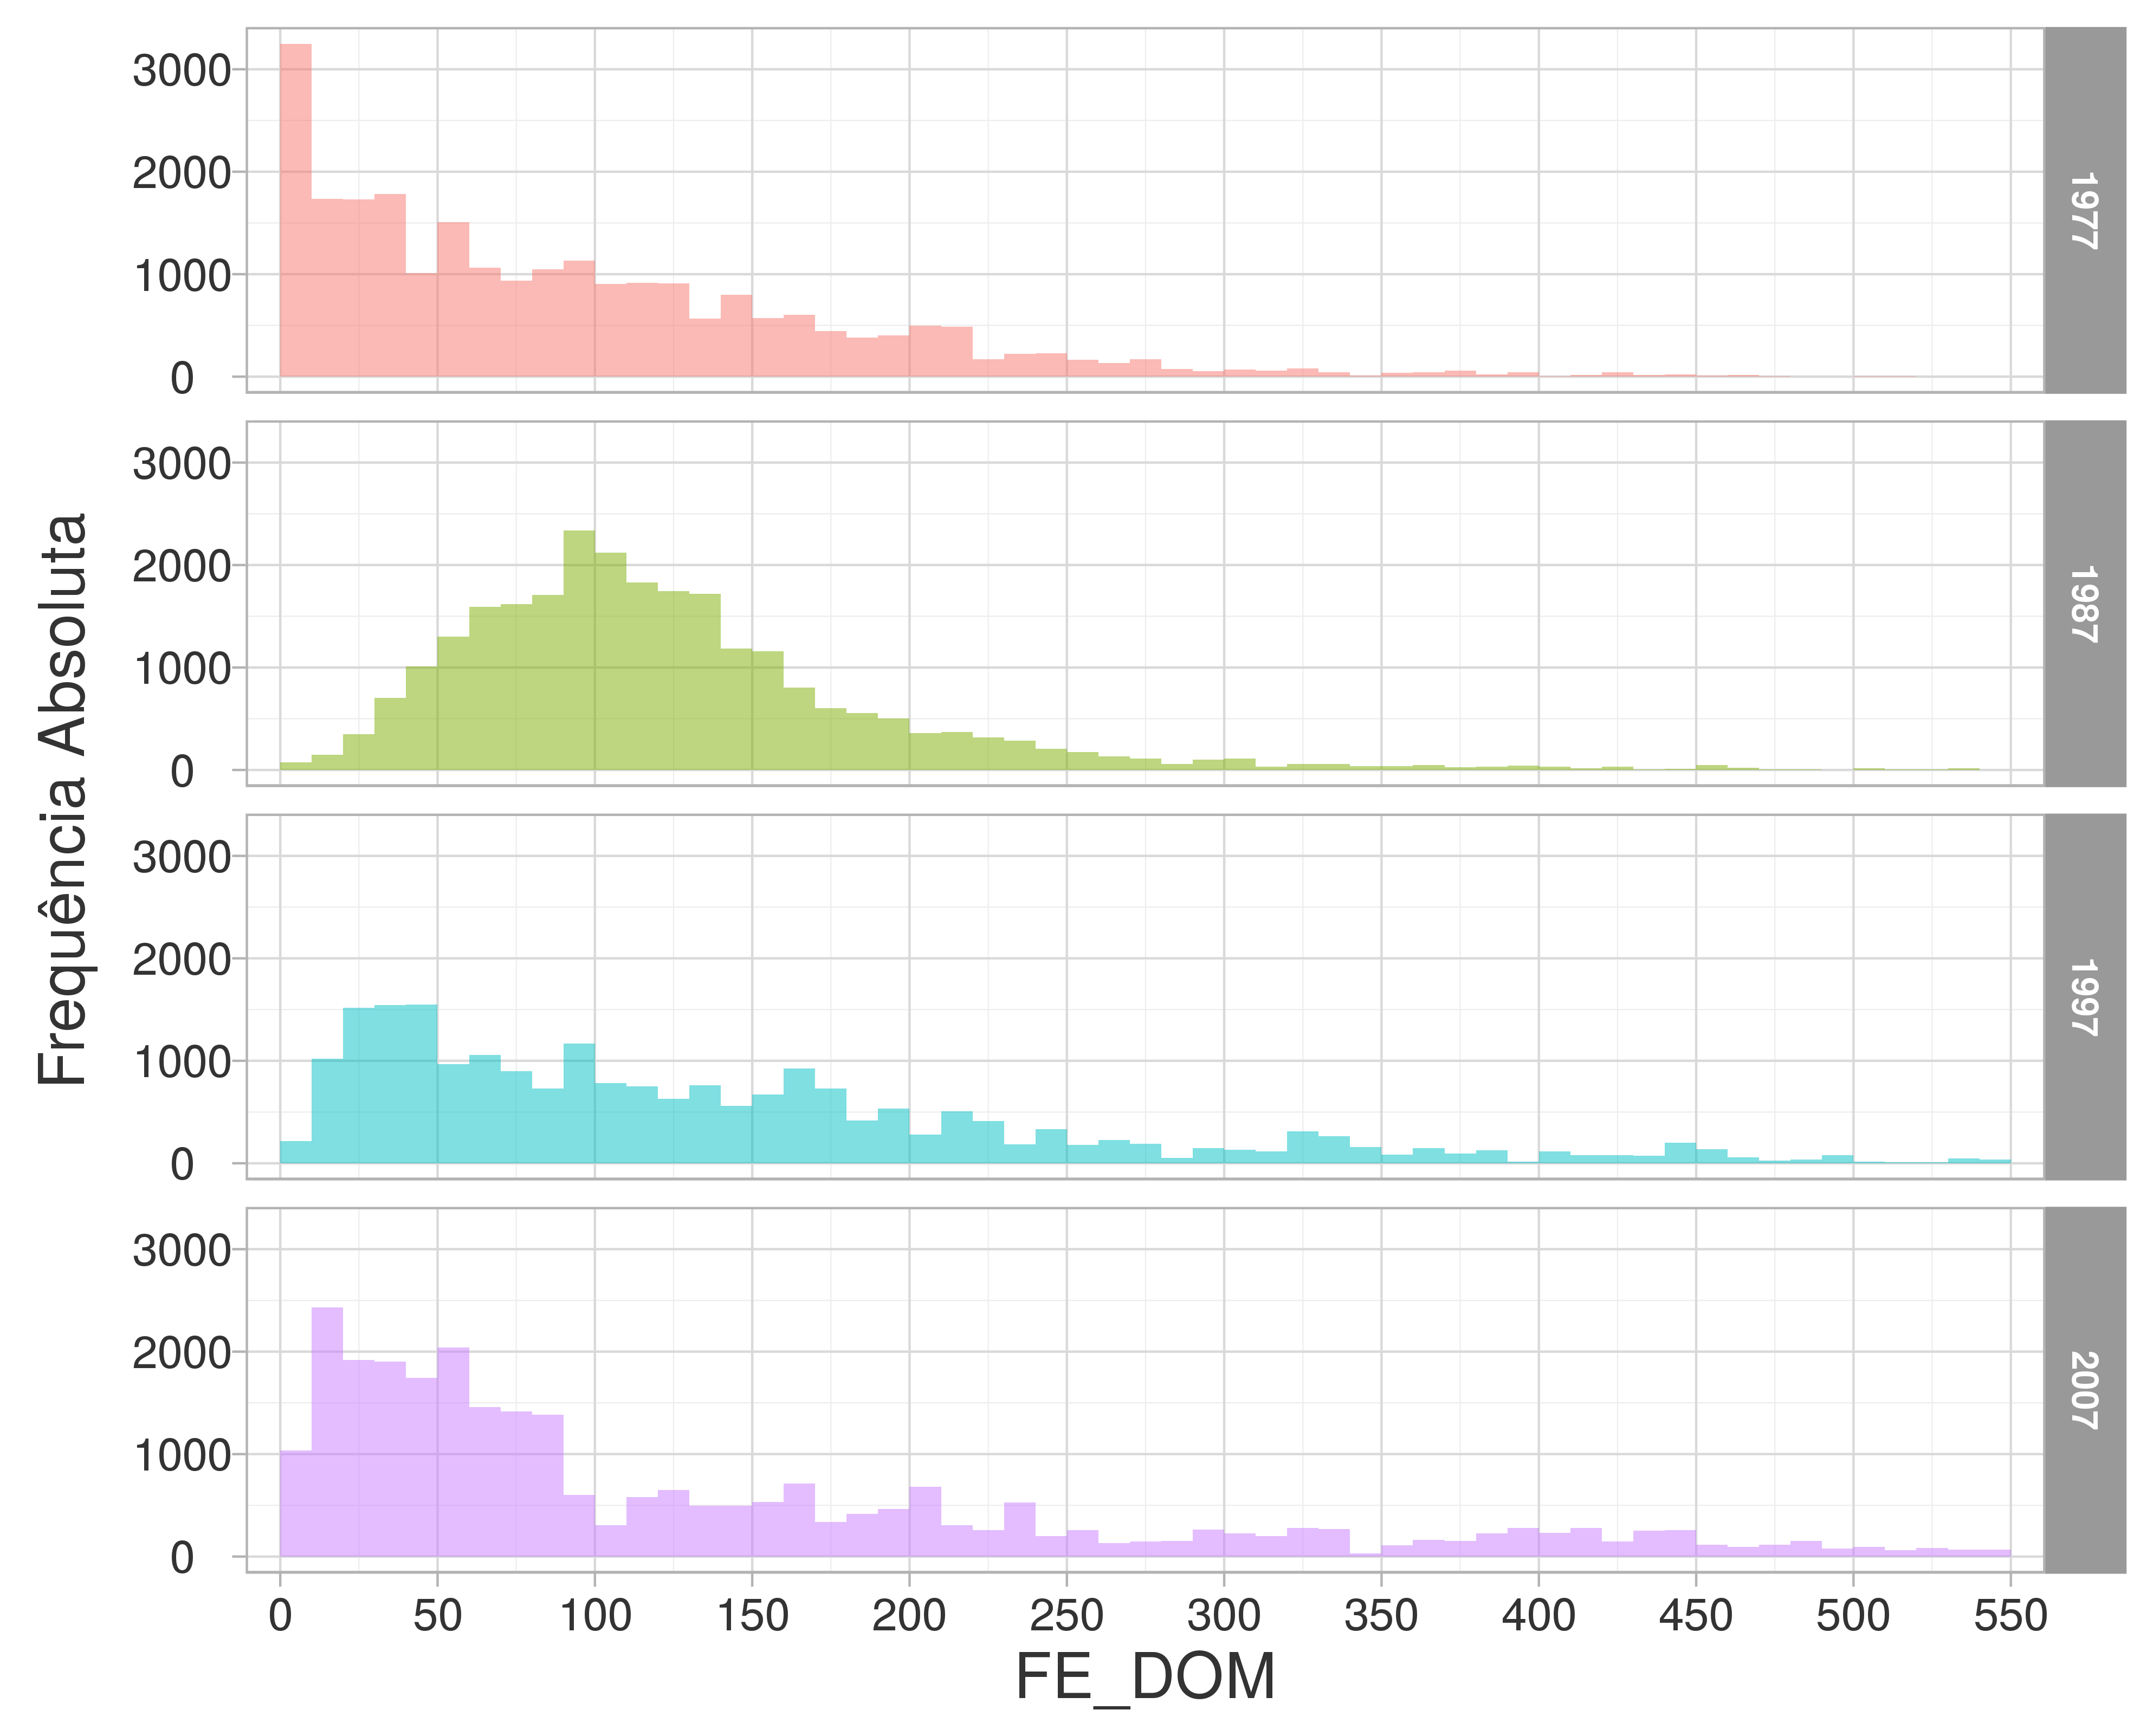
\includegraphics[width=1\textwidth]{./imagens/freq-abs-fe-dom.png}%
    \end{center}%
    %\fonte{Compilação própria}
\end{grafico}%


\clearpage

%\begin{table}[htb]
%\centering
%   \IBGEtab{%\renewcommand{\arraystretch}{1.5}%%\ABNTEXfontereduzida%
%        \renewcommand{\arraystretch}{1.5}
%        \caption{Estatísticas da variável ``FE_FAM''}
%        \label{tab:estat-fe-fam}
%    }{%
%
%    \begin{tabular}{cccccc}
%        \toprule
%        \textbf{ANO} & \textbf{Mínimo} & \textbf{1º Quartil} & \textbf{Mediana} & \textbf{3º Quartil} & \textbf{Máximo}  \\ \midrule \midrule
%        \textbf{1977}  & 0,50 & 24,77 &  68,49 & 137,90 & 1562,75 \\ \hline
%        \textbf{1987}  & 0,00 & 78,62 & 110,93 & 151,20 & 2210,00 \\ \hline
%        \textbf{1997}  & 1,00 & 49,26 & 109,54 & 200,05 & 2513,93 \\ \hline
%        \textbf{2007}  & 2,55 & 41,31 &  88,67 & 237,21 & 2256,41 \\ \hline
%        \textbf{Geral} & 0,00 & 48,00 &  99,37 & 172,85 & 2513,93 \\ \bottomrule
%        \textbf{ANO} & \textbf{Média} & \textbf{Desvio Padrão} & \textbf{Assimetria} & \textbf{Curtose} & \textbf{Nº de ``NA''}  \\ \midrule \midrule
%        \textbf{1977}  &  93,04 &  92,12 & 2,64 & 18,70 & 0 \\ \hline
%        \textbf{1987}  & 128,04 &  90,65 & 4,90 & 52,08 & 0 \\ \hline
%        \textbf{1997}  & 169,80 & 199,60 & 3,62 & 22,09 & 0 \\ \hline
%        \textbf{2007}  & 185,42 & 229,03 & 2,65 & 10,35 & 0 \\ \hline
%        \textbf{Geral} & 145,67 & 171,27 & 3,79 & 23,80 & 0 \\ \bottomrule
%        \end{tabular}
%    }
%
%\end{table}
%% Estatísticas para registros com F_FAM==1
%
%\begin{table}[htb]
%\centering
%   \IBGEtab{%\renewcommand{\arraystretch}{1.5}%%\ABNTEXfontereduzida%
%        \renewcommand{\arraystretch}{1.5}
%        \caption{Estatísticas da variável ``FE_PESS''}
%        \label{tab:estat-fe-pess}
%    }{%
%
%    \begin{tabular}{cccccc}
%        \toprule
%        \textbf{ANO} & \textbf{Mínimo} & \textbf{1º Quartil} & \textbf{Mediana} & \textbf{3º Quartil} & \textbf{Máximo}  \\ \midrule \midrule
%        \textbf{1977}  & 0,00 & 25,33 &  71,05 & 139,25 & 1562,75 \\ \hline
%        \textbf{1987}  & 0,00 & 79,46 & 111,78 & 151,24 & 2210,00 \\ \hline
%        \textbf{1997}  & 1,00 & 46,72 & 109,21 & 200,22 & 2516,28 \\ \hline
%        \textbf{2007}  & 2,92 & 48,25 & 111,45 & 296,24 & 2723,05 \\ \hline
%        \textbf{Geral} & 0,00 & 50,53 & 101,89 & 175,00 & 2723,05 \\ \bottomrule
%        \textbf{ANO} & \textbf{Média} & \textbf{Desvio Padrão} & \textbf{Assimetria} & \textbf{Curtose} & \textbf{Nº de ``NA''}  \\ \midrule \midrule
%        \textbf{1977}  &  95,10 &  94,15 & 2,76 & 20,84 & 0 \\ \hline
%        \textbf{1987}  & 128,58 &  90,56 & 4,78 & 49,15 & 0 \\ \hline
%        \textbf{1997}  & 170,00 & 203,37 & 3,69 & 23,14 & 0 \\ \hline
%        \textbf{2007}  & 213,72 & 260,38 & 2,81 & 12,60 & 0 \\ \hline
%        \textbf{Geral} & 148,76 & 177,83 & 4,14 & 29,04 & 0 \\ \bottomrule
%        \end{tabular}
%    }
%
%\end{table}
%% Estatísticas para registros com F_PESS==1

\clearpage
A variável \textbf{TIPO_DOM}, em 1977 e 1987, contava somente com as categorias particular e coletivo; já em 1997 e 2007 passou a existir também a categoria favela. Foram adotadas as categorias coletivo e particular, de forma que funcionasse como uma \textbf{dummy} indicativa de domicílio particular (1) ou não (0). Quem não respondeu foi tratado como ``NA'', encerrando 4 domicílios (23 registros) em 1987, conforme pode ser observado na Tabela \ref{tab:estat-tipo-dom}. Nota-se que o percentual de moradias unifamiliares sempre permaneceu, em média, superior a 90\%.

\begin{table}[htb]
\centering
   \IBGEtab{%\renewcommand{\arraystretch}{1.5}%%\ABNTEXfontereduzida%
        \renewcommand{\arraystretch}{1.5}
        \caption{Estatísticas da variável ``TIPO_DOM''}
        \label{tab:estat-tipo-dom}
    }{%

    \begin{tabular}{cccccc}
        \toprule
        \textbf{ANO} & \textbf{1977} & \textbf{1987} & \textbf{1997} & \textbf{2007} & \textbf{Total}\\ \midrule \midrule
        \textbf{TIPO\_DOM=0}       &    148 &    207 &  2.054 &  1.195 &   3.604 \\ \hline
        \textbf{TIPO\_DOM=1}       & 24.465 & 25.859 & 21.787 & 28.762 & 100.873 \\ \hline
        \textbf{TIPO\_DOM=``NA''}  &      0 &      4 &      0 &      0 &       4 \\ \bottomrule
        \end{tabular}
    }

\end{table}
% Estatísticas para registros com F_DOM==1

A variável \textbf{TOT_FAM}, um dado de contagem, indica quantas famílias existem no domicílio e tem suas estatísticas descritivas apresentadas na Tabela \ref{tab:estat-tot-fam}. O valor médio indica haver pouco mais de uma família por domicílio, sendo a maior média de 1997 - dado coerente com a menor porcentagem de domicílios individuais (~91\%) indicada pela variável TIPO_DOM. A Figura \ref{fig:box-plot-tot-fam} mostra que a influência dos \textit{outliers} diminui com o tempo, o que também se reflete na queda dos desvios padrão, que indica menor dispersão dos dados.


\begin{figure}[htb]%
    \caption{\label{fig:box-plot-tot-fam}Box plot da variável ``TOT_FAM'', por ano}%
    \begin{center}%
        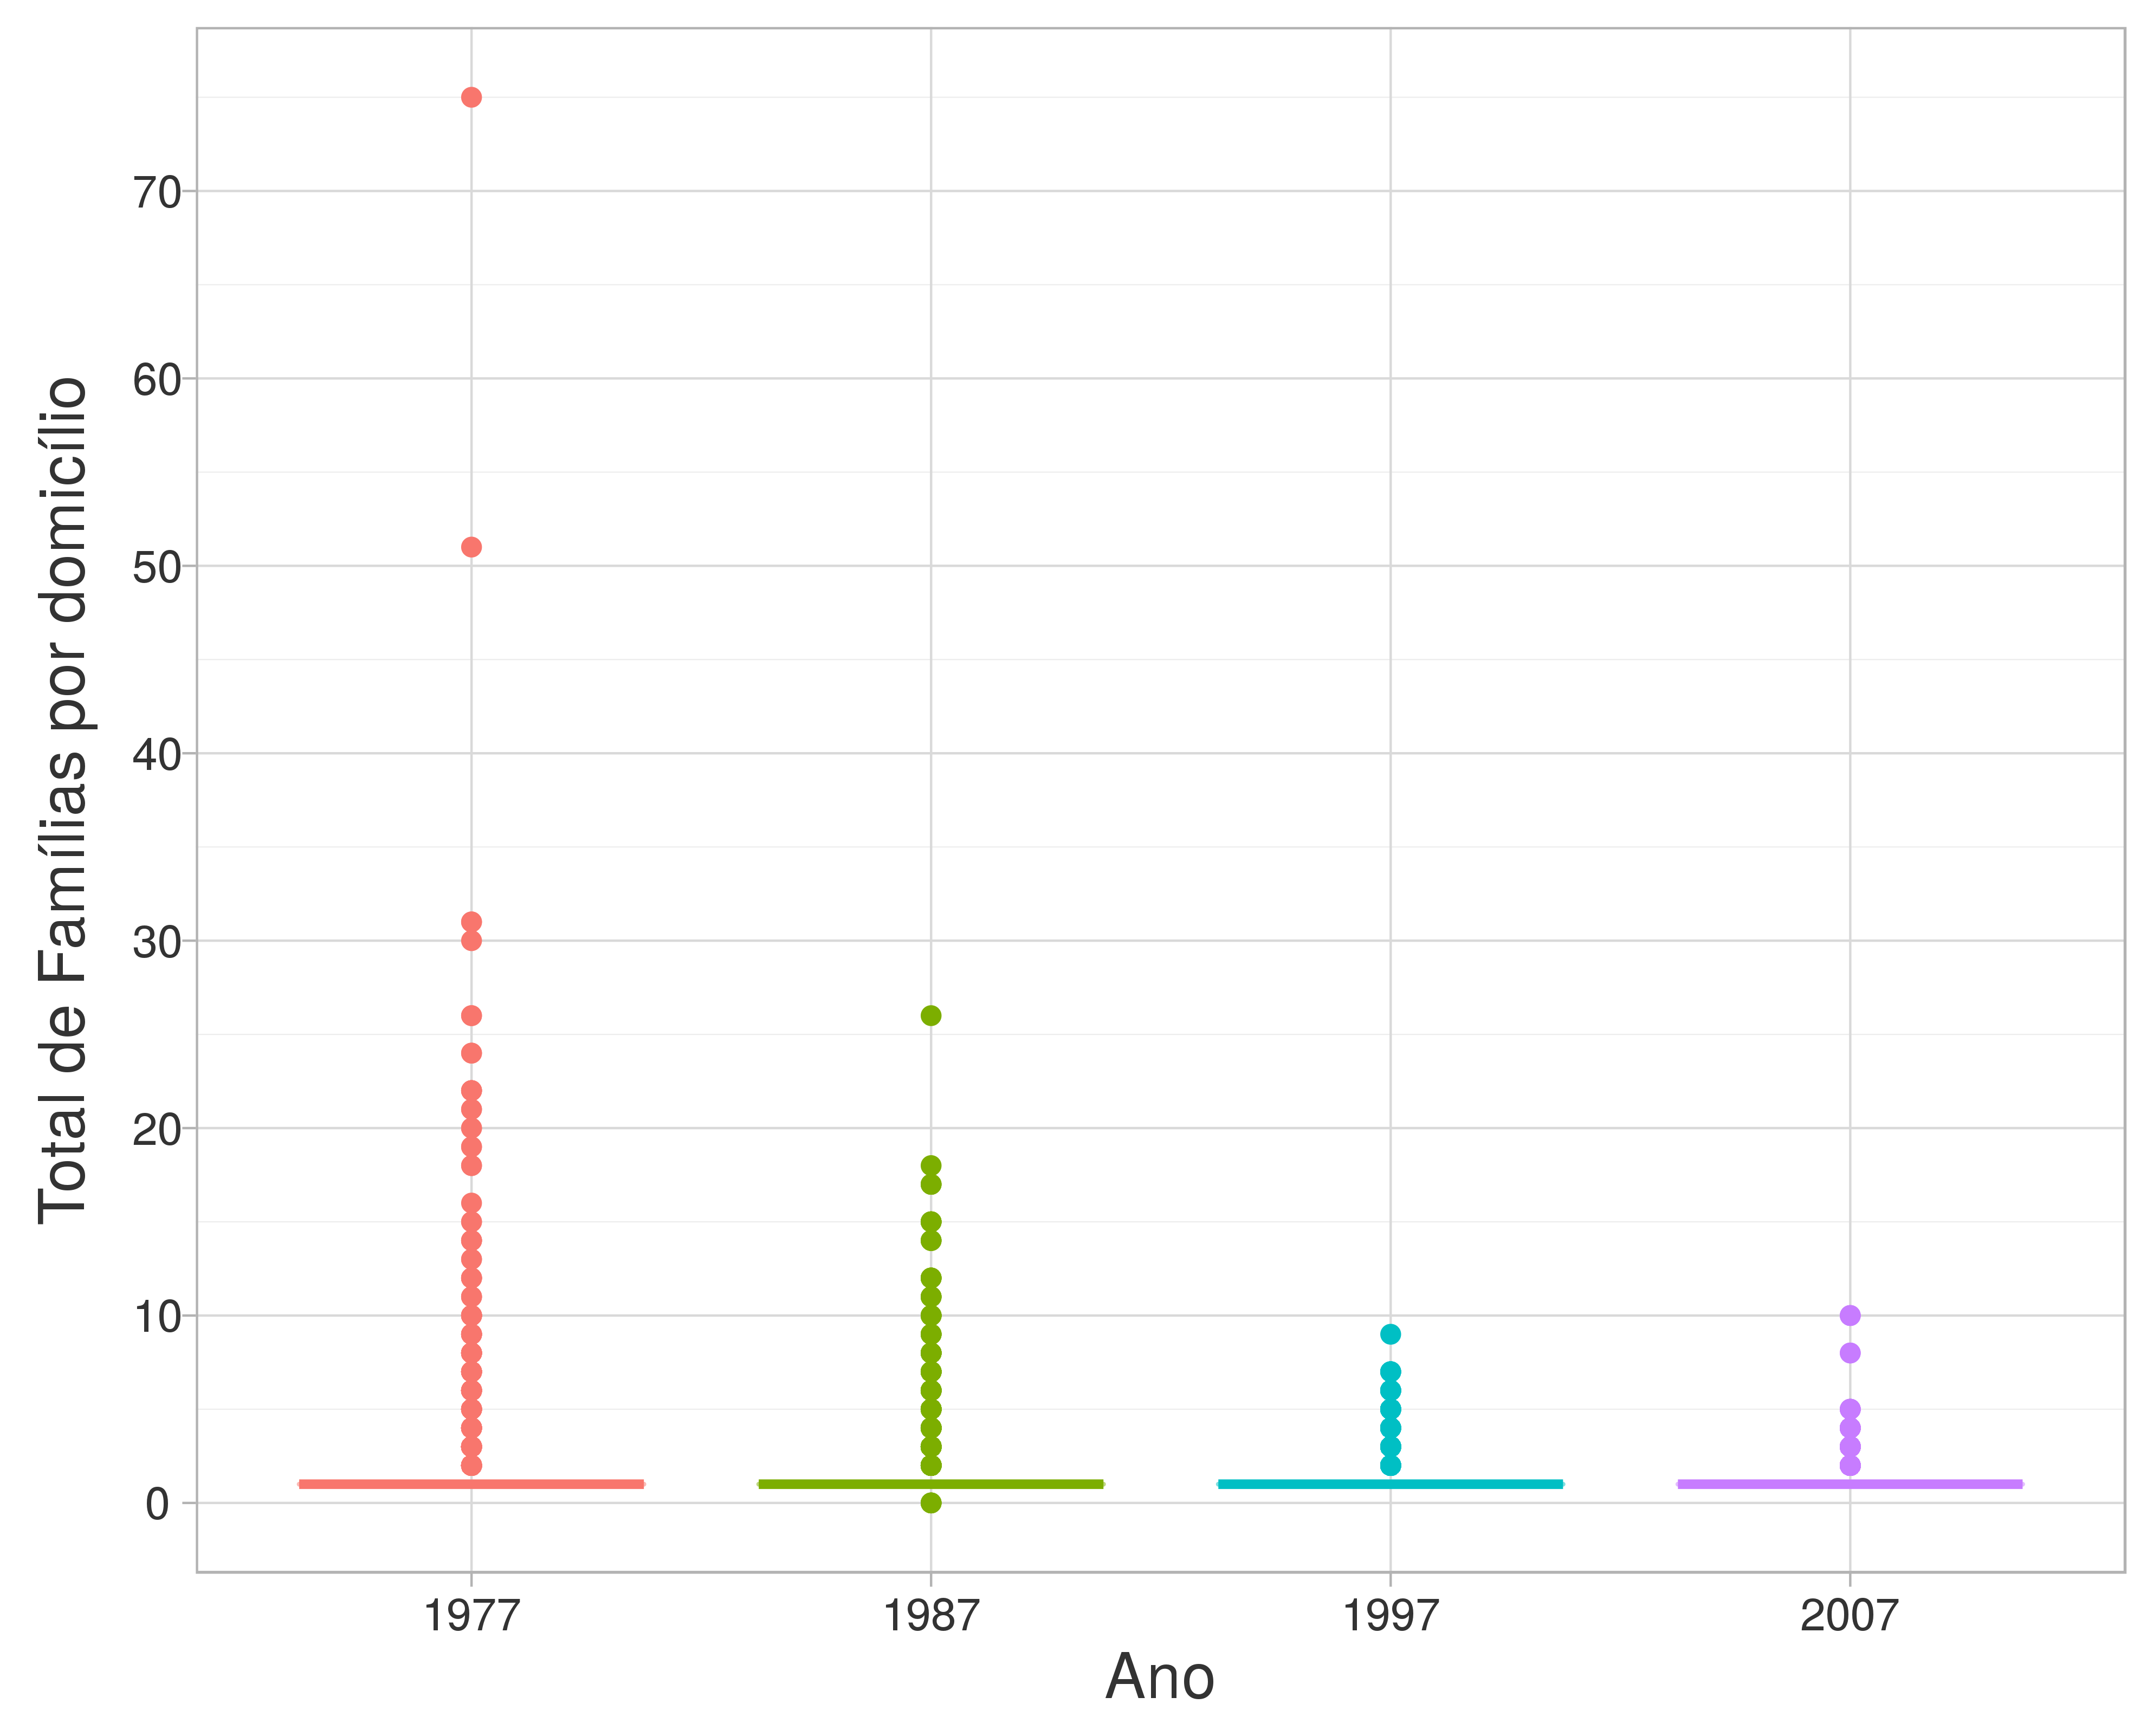
\includegraphics[width=1\textwidth]{./imagens/box-plot-tot-fam.png}%
    \end{center}%
    %\fonte{Compilação própria}
\end{figure}%

\begin{table}[htb]
\centering
   \IBGEtab{%\renewcommand{\arraystretch}{1.5}%%\ABNTEXfontereduzida%
        \renewcommand{\arraystretch}{1.5}
        \caption{Estatísticas da variável ``TOT_FAM''}
        \label{tab:estat-tot-fam}
    }{%

    \begin{tabular}{cccccc}
        \toprule
        \textbf{ANO} & \textbf{Média} & \textbf{Desvio Padrão} & \textbf{Assimetria} & \textbf{Curtose} & \textbf{Máximo}  \\ \midrule \midrule
        \textbf{1977}  & 1,08 & 0,99 & 33,70 & 1777,74 & 75 \\ \hline
        \textbf{1987}  & 1,12 & 0,61 & 13,72 & 306,37 & 26 \\ \hline
        \textbf{1997}  & 1,13 & 0,45 & 4,85 & 32,42 & 9 \\ \hline
        \textbf{2007}  & 1,03 & 0,23 & 14,00 & 346,13 & 10 \\ \hline
        \textbf{Geral} & 1,09 & 0,62 & 35,68 & 2734,92 & 75 \\ \bottomrule
        \end{tabular}
    }

\end{table}
% Estatísticas para registros com F_DOM==1


\newpage 

A variável \textbf{COND_MORA}, de natureza qualitativa, conta com três valores únicos, cujas frequências absolutas de registros são apresentada na Tabela \ref{tab:estat-cond-mora}. 
A categoria ``alugada'' (1) que em 1977 representava ~35\% da amostra, caiu para 23\% em 2007. A posse de residência (categoria ``própria'' - 2), subiu de 57\% para 68\% da amosta anual. A categoria ``outros'' (3), que abarca as categorias originais ``cedida'', ``outros'' e ``não se aplica'', oscila numa faixa próxima dos 10\%. Quem não respondeu foi tratado como ``NA'', encerrando 717 domicílios: 9 em 1977, 264 em 1987, 26 em 1997 e 460 em 2007.

\begin{table}[htb]
    \IBGEtab{%\renewcommand{\arraystretch}{1.5}%%\ABNTEXfontereduzida%
        \renewcommand{\arraystretch}{1.5}
        \caption{Estatísticas da variável ``COND_MORA''}
        \label{tab:estat-cond-mora}
    }{%

    \begin{tabular}{cccccc}
        \toprule
        \textbf{ANO} & \textbf{1977} & \textbf{1987} & \textbf{1997} & \textbf{2007} & \textbf{Total}\\ \midrule \midrule
        \textbf{COND_MORA=1}      &  9.174 &  7.967 &  5.168 &  7.268 & 29.577 \\ \hline
        \textbf{COND_MORA=2}      & 14.984 & 17.429 & 18.040 & 21.062 & 71.515 \\ \hline
        \textbf{COND_MORA=3}      &  1.990 &  2.557 &  3.611 &  1.830 &  2.065 \\ \hline
        \textbf{COND_MORA=``NA''} &      9 &    264 &     26 &    460 &    759 \\ \bottomrule
        \end{tabular}
    }

\end{table}
% Estatísticas para registros com F_FAM==1


Não foram mantidas no BDU as variáveis relativas aos bens de consumo, pois a função delas era servir de \emph{input} para determinar a renda atribuída (na ausência de declaração da renda), informação de que já se dispõe no banco de dados. Apenas os bens que são meios de transporte foram mantidos (automóveis, motocicletas e bicicletas) e serão explorados mais adiante.

Os valores monetários de renda familiar, renda individual e valor de estacionamento encontravam-se, em cada banco de dados, em um mês de referência diferente (segundo Quadro \ref{qua:atrib-renda}). Foram estudadas as possibilidades de correção pelos seguintes índices:

\begin{compactitem}
\item IPC-Brasil: índice de preços ao consumidor, que mede a variação de preços de um conjunto fixo de bens e serviços componentes de despesas habituais de famílias com nível de renda situado entre 1 e 33 salários mínimos mensais. Sua pesquisa de preços se desenvolve diariamente, cobrindo as sete principais capitais do país. Suas variações (DI, M e 10) referem-se ao período da coleta dos preços. A série histórica que se obteve de fontes oficiais (página da FGV e do Banco Central) não disponibilizava valores anteriores a 1989.

\item IGP: índice geral de preços, (a partir de 1950) é a média aritmética ponderada de três outros índices de preços (desde : Índice de Preços ao Produtor Amplo (50\%), Índice de Preços ao Consumidor (30\%) e Índice Nacional de Custo da Construção (10\%). O IGP-M/FGV se refere ao período do dia vinte e um do mês anterior ao dia vinte do mês de referência e o IGP-DI/FGV se refere ao período do dia um ao dia trinta do mês em referência. A série histórica que se obteve de fontes oficiais (página da FGV e do Banco Central) não disponibilizava valores anteriores a 1989 para o IGP-M, ao passo que o IGP-DI
\footnote{Metodologia do IGP-DI disponível em: \url{http://portalibre.fgv.br/lumis/portal/file/fileDownload.jsp?fileId=8A7C82C54DB5CA9F014DD9322ADD306E} Acesso em 30 de agosto de 2015} dispunha de valores para correção desde a década de 1940.

\item IPCA: índice geral de preços ao consumidor amplo, que mede a variação de preços de um conjunto fixo de bens e serviços componentes de despesas habituais de famílias com nível de renda situado entre 1 e 40 salários mínimos mensais. Sua pesquisa de preços se desenvolve diariamente, cobrindo as dez principais capitais do país e Brasília. A série histórica que se obteve de fontes oficiais (página do IBGE e do Banco Central) divulga valores após dezembro de 1979. Sua variação IPCA-E é ainda mais recente (1991) e tem divulgação trimestral.

\item INPC: índice nacional de preços ao consumidor amplo, que mede a variação de preços de um conjunto fixo de bens e serviços componentes de despesas habituais de famílias com nível de renda situado entre 1 e 5 salários mínimos mensais. Sua pesquisa de preços se desenvolve continuamente, cobrindo as dez principais capitais do país e Brasília. A série histórica que se obteve de fontes oficiais (página do IBGE e do Banco Central) divulga valores após março de 1979.

\end{compactitem}

Assim, pela abrangência histórica foi utilizado o IPG-DI para levar os valores de setembro de 1977 para setembro de 1987. Estes valores, bem como os advindos da OD de 1987, foram levados a outubro de 2007 sofrendo correção do INPC. Este mesmo índice foi utilizado para levar os valores de outubro de 1997 a outubro de 2007. Escolheu-se o INPC, dentro os demais disponíveis, devido à faixa de abrangência da renda familiar utilizada em sua determinação. Não se quis priorizar índices cujas cestas tivessem um perfil de consumo alto, dado que as politicas de transporte público devem priorizar especialmente as menores faixas de renda. A composição final dos deflatores utilizados é apresentada na Tabela \ref{tab:deflatores}.

\begin{table}[htb]
    \IBGEtab{%\renewcommand{\arraystretch}{1.5}%%\ABNTEXfontereduzida%
        \renewcommand{\arraystretch}{1.5}
        \caption{Deflatores utilizados para correção dos valores monetários para outubro/2007}
        \label{tab:deflatores}
    }{%

    \begin{tabular}{ccccc}
        \toprule
        \textbf{ANO} & \textbf{1977} & \textbf{1987} & \textbf{1997} & \textbf{2007}\\ \midrule \midrule
        \textbf{Deflator} & 0,44234590 & 0,09664666 & 1,94136464 & 1  \\ \bottomrule
        \end{tabular}
    }

\end{table}


A renda familiar (variável \textbf{REN_FAM}) tem seus maiores de média e mediana em 1977, conforme Tabela \ref{tab:estat-ren-fam}, talvez por reflexo da época do ``milagre econômico brasileiro'', %TODO por referencia aqui 
comumente atribuído ao período do final dos anos 1960 até a metade dos anos 1970.
Após isso, 1987 apresenta a menor média e também queda da mediana, pode ser devido à recessão que marcou o Brasil nos anos 1980, quando se registraram baixo crescimento do PIB, %TODO por referencia aqui
alto nível de desemprego, %TODO por referencia aqui
perda do poder de compra da população, %TODO por referencia aqui 
e índices de inflação extremamente elevados. %TODO por referencia aqui
Em 1997, as média da renda familiar sobe, porém a mediana continua a cair, o que pode significar uma recuperação do aquecimento econômico, porém, sem frear o aprofundamento das desigualdades. %TODO por referencia aqui
Com o valor da média de 2007, parece realmente estar ocorrendo uma recuperação econômica (aumento da renda média familiar) e também uma redução das desigualdades (aumento da mediana da renda média familiar) - ver Gráfico \ref{graf:freq-rel-ren-fam}.


\begin{table}[htb]
\centering
   \IBGEtab{%\renewcommand{\arraystretch}{1.5}%%\ABNTEXfontereduzida%
        \renewcommand{\arraystretch}{1.5}
        \caption{Estatísticas da variável ``REN_FAM''}
        \label{tab:estat-ren-fam}
    }{%
    \begin{tabular}{cccccc}
        \toprule
        \textbf{ANO} & \textbf{Mínimo} & \textbf{1º Quartil} & \textbf{Mediana} & \textbf{3º Quartil} & \textbf{Máximo}  \\ \midrule \midrule
        \textbf{1977}  & 0 & 1.351,51 & 2.534,08 & 4.796,58 &  42.234,2 \\ \hline
        \textbf{1987}  & 0 &   875,62 & 1.523,44 & 2.801,21 &  61.830,1 \\ \hline
        \textbf{1997}  & 0 &   330,03 & 1.203,65 & 2.912,05 & 172.781,0 \\ \hline
        \textbf{2007}  & 0 & 1.144,82 & 2.080,00 & 4.000,00 &  46.000,0 \\ \hline
        \textbf{Geral} & 0 &   935,73 & 1.801,63 & 3.582,21 & 172.181,0 \\ \bottomrule
        \textbf{ANO} & \textbf{Média} & \textbf{Desvio Padrão} & \textbf{Assimetria} & \textbf{Curtose} & \textbf{Nº de ``NA''}  \\ \midrule \midrule
        \textbf{1977}  & 4.037,27 & 4.724,88 & 3,56 &  18,74 & 0 \\ \hline
        \textbf{1987}  & 2.393,58 & 2.826,96 & 4,06 &  29,85 & 0 \\ \hline
        \textbf{1997}  & 2.453,89 & 4.148,06 & 7,20 & 149,78 & 0 \\ \hline
        \textbf{2007}  & 3.186,19 & 3.312,25 & 2,85 &  13,73 & 0 \\ \hline
        \textbf{Geral} & 3.009,86 & 3.845,58 & 4,74 &  63,49 & 0 \\ \bottomrule
        \end{tabular}
    }

\end{table}
% Estatísticas para registros com F_FAM==1

\begin{grafico}[htb]%
    \caption{\label{graf:freq-rel-ren-fam}Distribuição da variável ``REN_FAM'', por ano}%
    \begin{center}%
        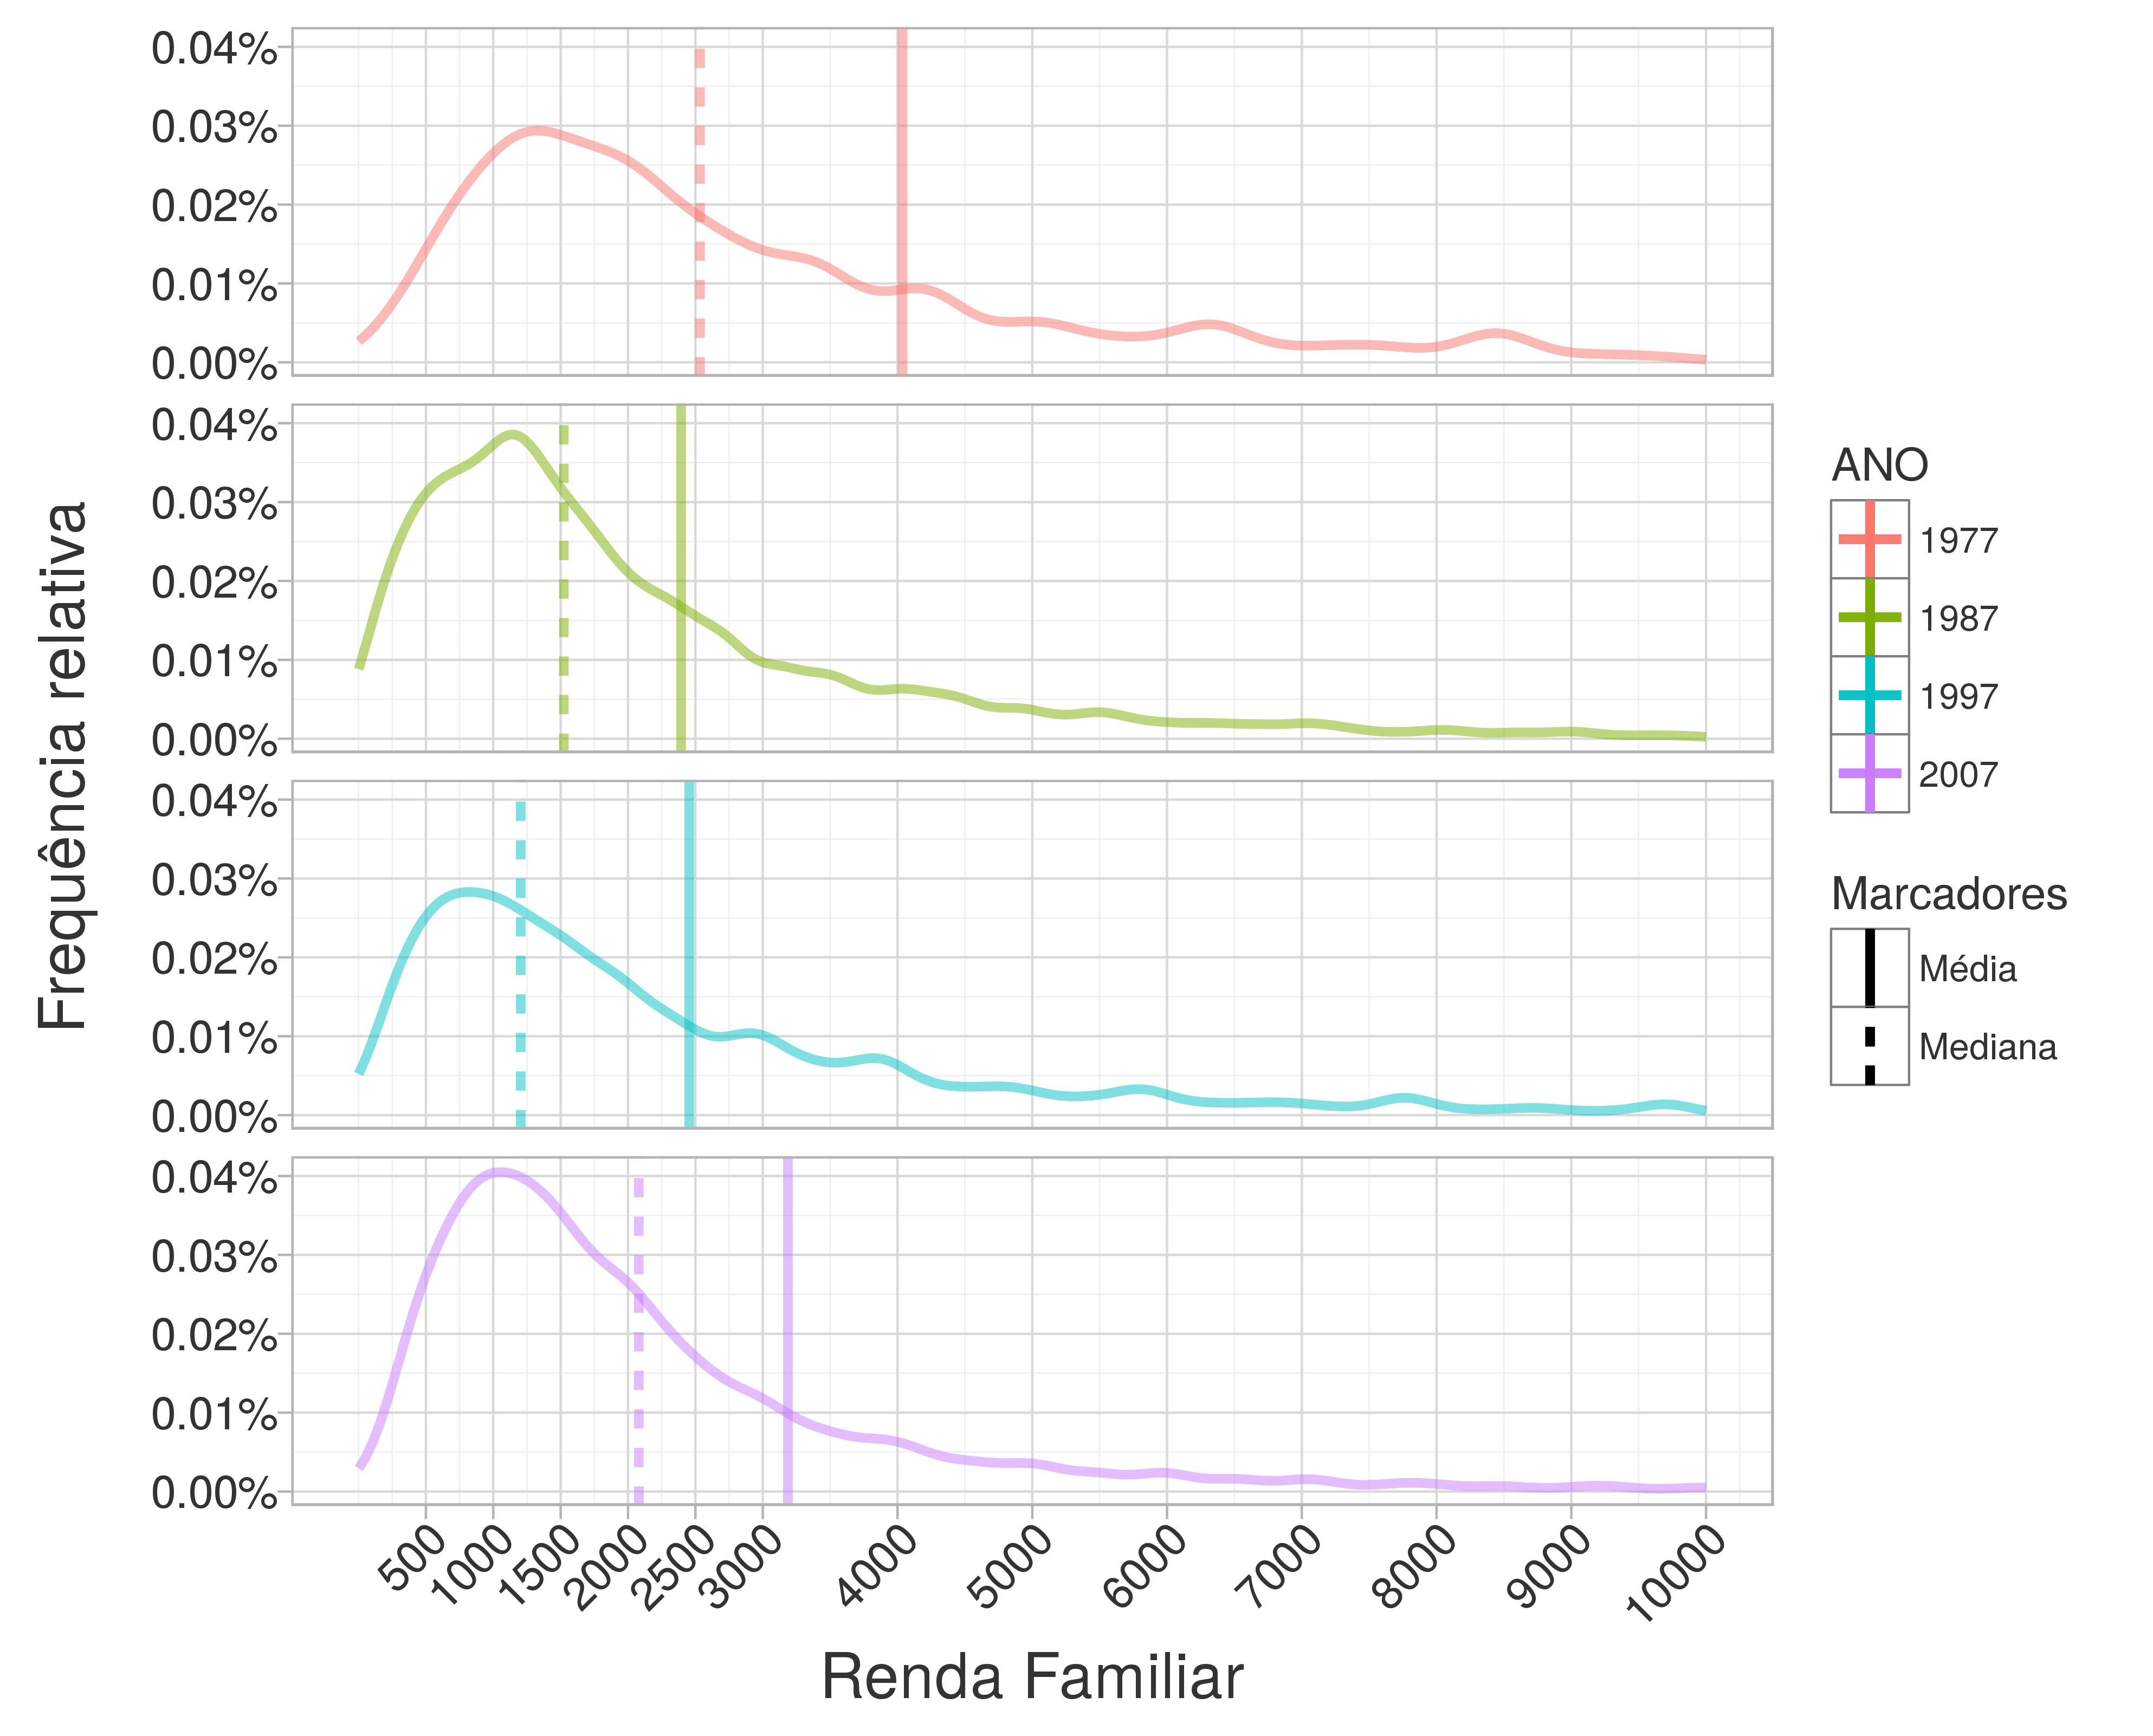
\includegraphics[width=1\textwidth]{./imagens/freq-rel-ren-fam.png}%
    \end{center}%
    %\fonte{Compilação própria}
\end{grafico}%

Para a construção do Gráfico \ref{graf:class-econ-ren-fam}, a partir da variável \textbf{FAIXA_REN_FAM}, foram retiradas as famílias que declararam renda nula. Posto isso, vê-se que as classes E e D, em 1977, correspondiam a 29\% da amostra. Em 1987 esse valor vai a 49\% e depois começa a decrescer para 45\% em 1997 e 37\% em 2007. A classe C (classe média) decresce de 1977 (~37\%) até 1997 (~33\%) e só aumenta novamente em 2007 (~36\%). Para estas classificações, foram utilizados sempre os valores em R\$ de outubro de 2007, bem como a classificação de classes econômicas vigente neste mesmo período.

\begin{grafico}[htb]%
    \caption{\label{graf:class-econ-ren-fam}Distribuição da variável ``FAIXA_REN_FAM'', por ano}%
    \begin{center}%
        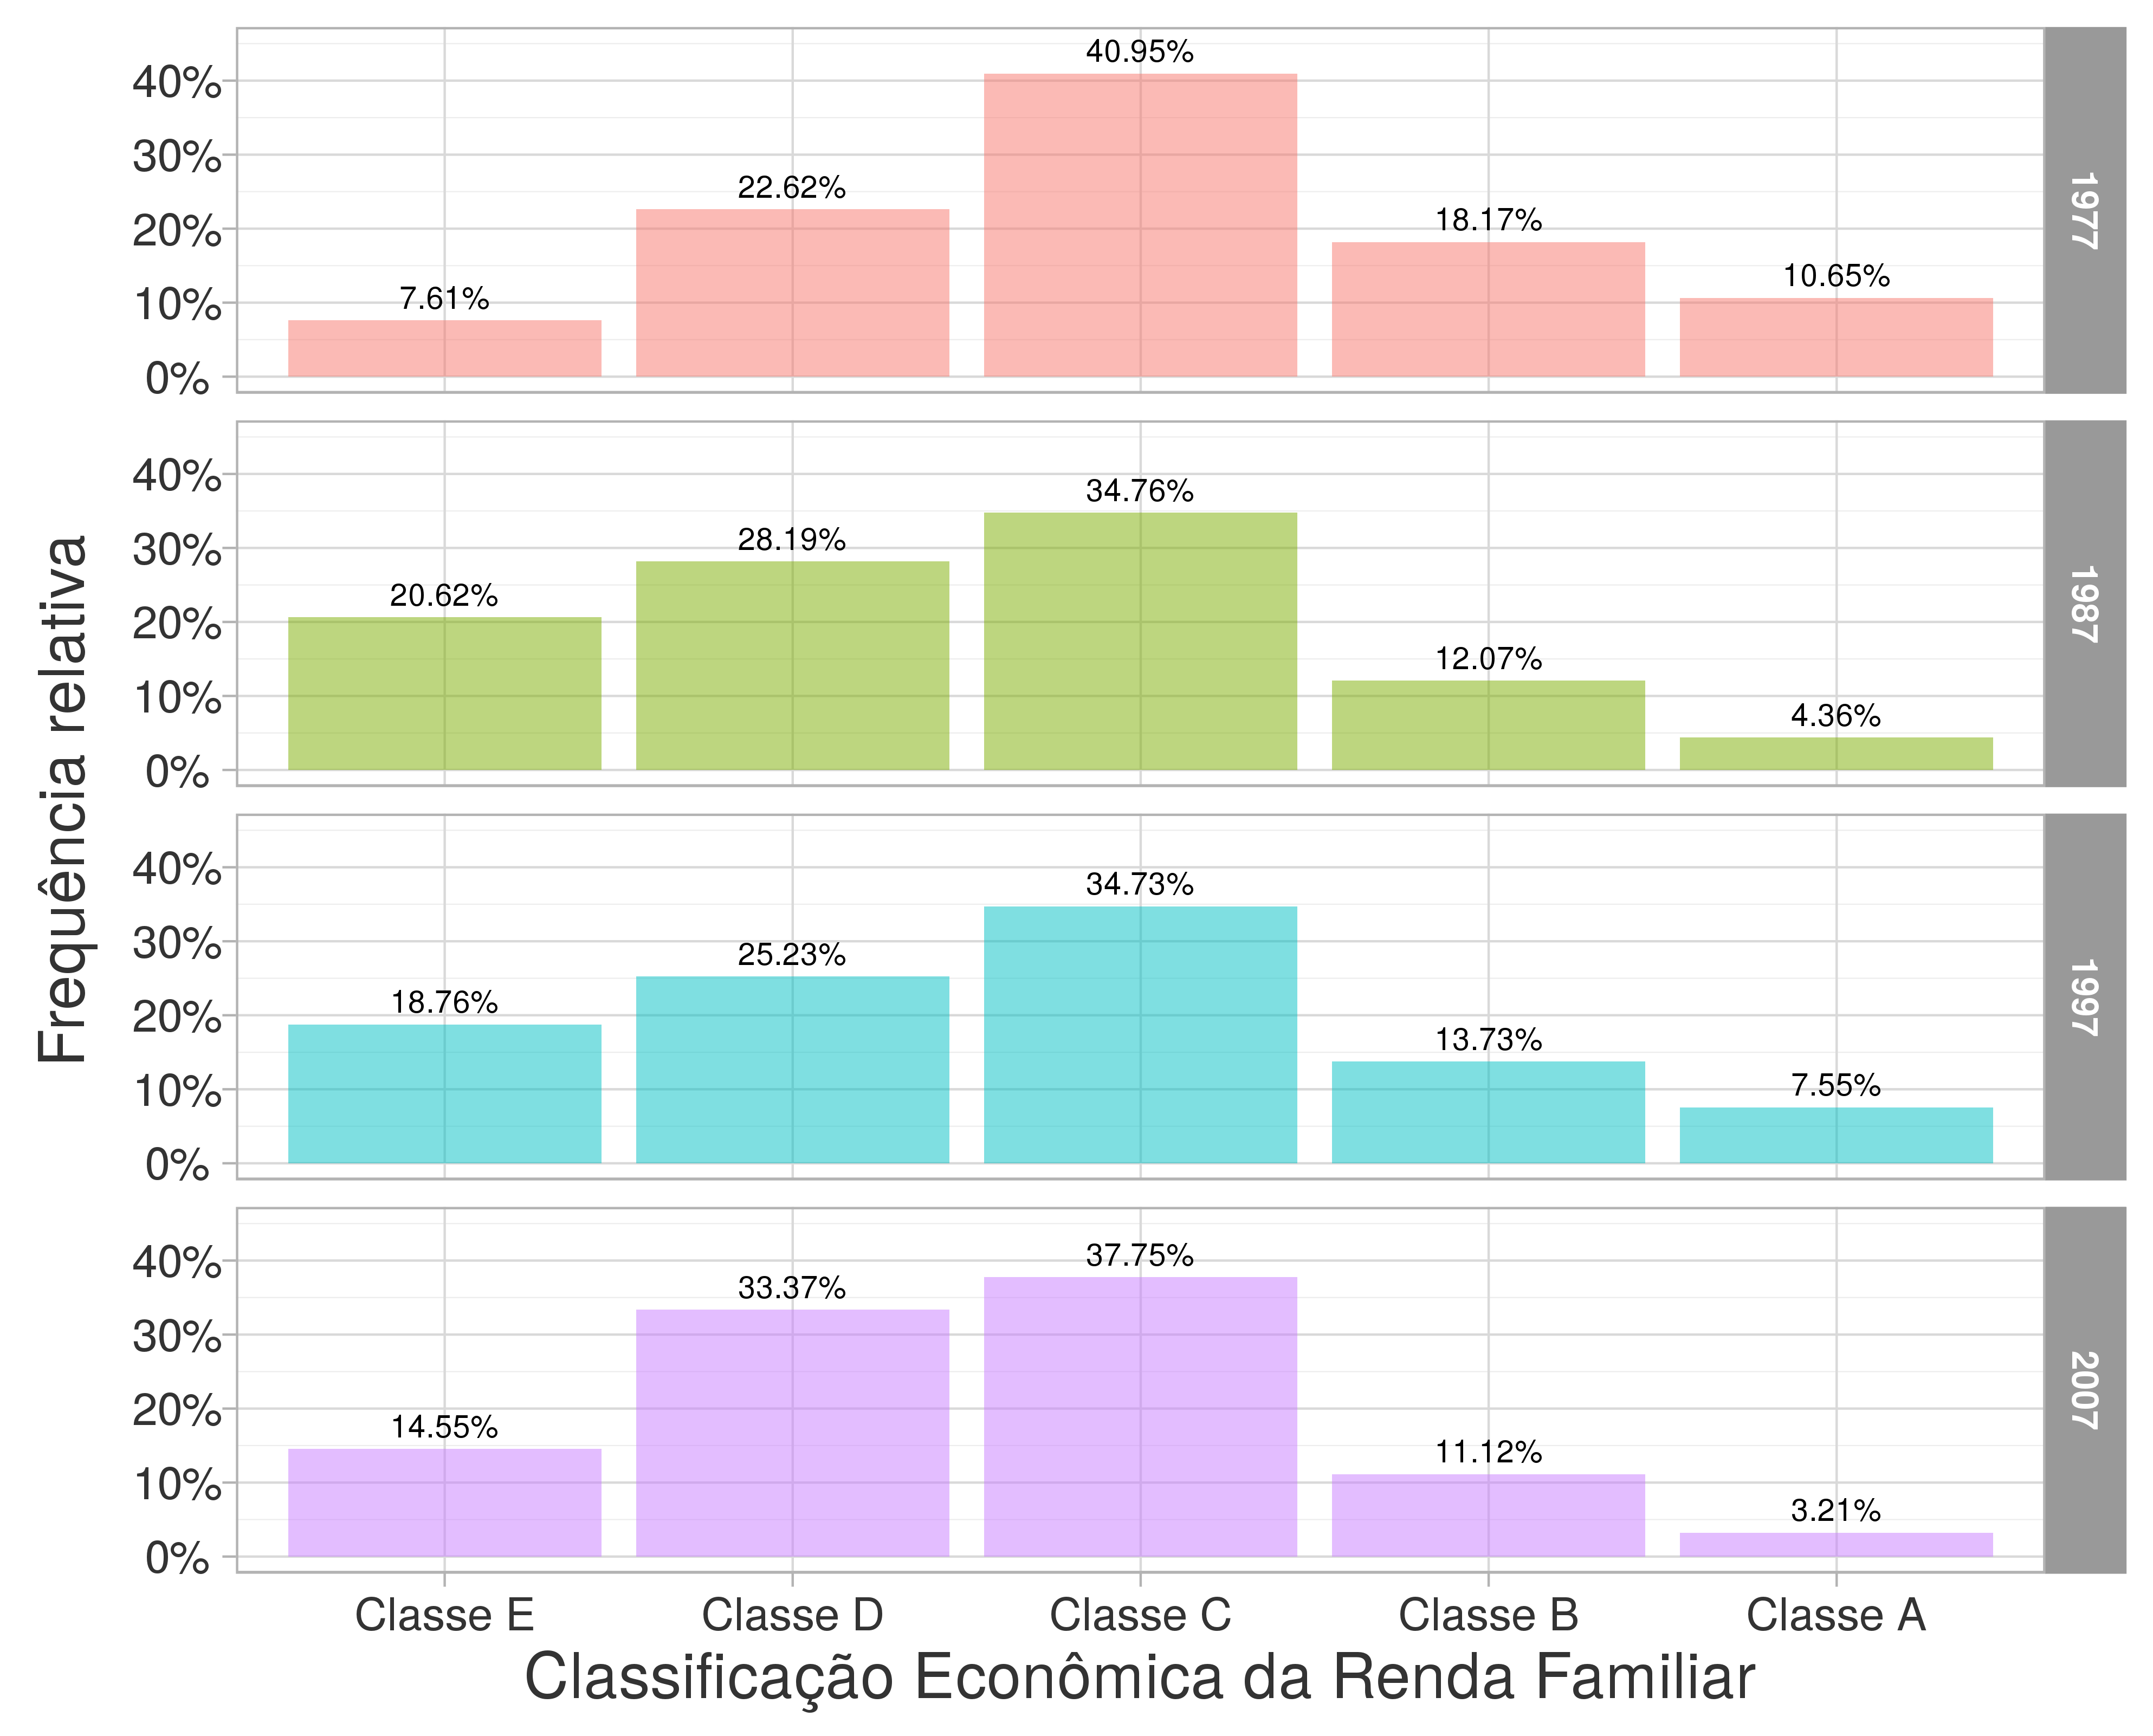
\includegraphics[width=1\textwidth]{./imagens/class-econ-ren-fam.png}%
    \end{center}%
    %\fonte{Compilação própria}
\end{grafico}%

\newpage

Uma das variáveis que são \textit{proxy} da renda é a quantidade de automóveis na família (\textbf{QT_AUTO}).
As Tabelas \ref{tab:estat-frota} e \ref{tab:venda-veic-br} mostram que a frota de automóveis de uso familiar vem crescendo tanto no Brasil como na RMSP, assim como a motorização familiar (número de veículos por família) ao longo do tempo. Isto é, mesmo com o crescimento populacional do período, a aquisição de carros pelas famílias aumenta em taxa ainda maior.
A média de automóveis por família aumentou com o passar do tempo, conforme observa-se na coluna \textit{média} da Tabela \ref{tab:estat-qt-auto}.

\begin{table}[htb]
    \IBGEtab{%\renewcommand{\arraystretch}{1.5}%%\ABNTEXfontereduzida%
        \renewcommand{\arraystretch}{1.5}
        \caption{Evolução da frota de automóveis na RMSP segundo as Pesquisas OD}
        \label{tab:estat-frota}
    }{%

    \begin{tabular}{ccccc}
        \toprule
        \textbf{ANO} & \textbf{1977} & \textbf{1987} & \textbf{1997} & \textbf{2007}\\ \midrule \midrule
        \textbf{Frota} & 1.391.832 & 2.014.474 & 3.092.238 & 3.545.263  \\ \bottomrule
        \end{tabular}
    }

    \nota{Segundo o Departamento Estadual de Trânsito de São Paulo, em 2007 o município de São Paulo contava com cerca de 4,5milhões de automóveis (Fonte: \url{http://www.detran.sp.gov.br/wps/wcm/connect/1eb3cf81-624b-4a71-b626-317730638e74/\%28Frota\%2B2008\%29.pdf?MOD=AJPERES&CACHEID=1eb3cf81-624b-4a71-b626-317730638e74}). Tal discrepância pode ocorrer porque as Pesquisas OD domiciliares tem seu número de viagens aferido (FE_VIAG deduzido) pelas viagens feitas realizadas nos sistemas de transportes de massa.}
    
\end{table}

\begin{table}[htb]
    \IBGEtab{%\renewcommand{\arraystretch}{1.5}%%\ABNTEXfontereduzida%
	    \renewcommand{\arraystretch}{1.5}
        \caption{Venda interna de veículos no Brasil entre 1960 e 2009}
		\label{tab:venda-veic-br}
    }{%
	    \begin{tabular}{p{2.00cm} P{4.0cm} P{4.0cm} P{4.0cm}}
            \toprule
	           \headerTabCenterCell{Ano} &
		       \headerCell{Autos} &
		       \headerCell{Total} &
		       \headerCell{Fator de crescimento (total)} \\
		    \midrule \midrule
		        1960&
		        40.980&
		        131.499&
		        1\\
		    \midrule
		        1970&
		        308.024&
		        416.704&
		        3,2\\
		    \midrule
		        1980&
		        739.028&
		        980.261&
		        7,5\\
		    \midrule
		        1990&
		        532.906&
		        712.741&
		        5,4\\
		    \midrule
		        2000&
		        1.176.774&
		        1.489.481&
		        11,3\\
		    \midrule
		        2009&
		        2.474.764&
		        3.141.240&
		        23,9\\
		    \bottomrule
		\end{tabular}
    }{%
		\fonte{Adaptado de \cite[p.29]{VASCONCELLOS2012}}
		}
\end{table}


\begin{table}[htb]
\centering
   \IBGEtab{%\renewcommand{\arraystretch}{1.5}%%\ABNTEXfontereduzida%
        \renewcommand{\arraystretch}{1.5}
        \caption{Estatísticas da variável ``QT_AUTO''}
        \label{tab:estat-qt-auto}
    }{%

    \begin{tabular}{cccccc}
        \toprule
        \textbf{ANO} & \textbf{Mínimo} & \textbf{1º Quartil} & \textbf{Mediana} & \textbf{3º Quartil} & \textbf{Máximo}  \\ \midrule \midrule
        \textbf{1977}  & 0 & 0 & 0 & 1 & 7 \\ \hline
        \textbf{1987}  & 0 & 0 & 0 & 1 & 9 \\ \hline
        \textbf{1997}  & 0 & 0 & 1 & 1 & 9 \\ \hline
        \textbf{2007}  & 0 & 0 & 1 & 1 & 8 \\ \hline
        \textbf{Geral} & 0 & 0 & 0 & 1 & 9 \\ \bottomrule
        \textbf{ANO} & \textbf{Média} & \textbf{Desvio Padrão} & \textbf{Assimetria} & \textbf{Curtose} & \textbf{Nº de ``NA''}  \\ \midrule \midrule
        \textbf{1977}  & 0,65 & 0,81 & 1,36 & 2,28 & 0 \\ \hline
        \textbf{1987}  & 0,57 & 0,77 & 1,59 & 4,09 & 0 \\ \hline
        \textbf{1997}  & 0,72 & 0,89 & 1,57 & 3,78 & 0 \\ \hline
        \textbf{2007}  & 0,78 & 0,86 & 1,19 & 1,99 & 0 \\ \hline
        \textbf{Geral} & 0,68 & 0,84 & 1,43 & 3,03 & 0 \\ \bottomrule
        \end{tabular}
    }

\end{table}
% Estatísticas para registros com F_FAM==1

Diversos estudos foram realizados para a construção de modelos desagregados que explicassem a posse de autos
\cite{RYAN1999, DARGAY1999, DARGAY2001, CHU2002, KARLAFTIS2002, PFEIFFER2005}.
É comum a utilização de variáveis como renda, número de trabalhadores, tamanho da família, número de estudantes, presença ou não de crianças na família, sexo e idade da pessoa responsável pela família. Embora não seja o foco deste estudo modelar a posse de autos pelas famílias, compreender o que influencia a motorização é importante porque a motorização influencia diretamente a mobilidade dos indivíduos.
\citeauthoronline{PFEIFFER2005} (\citeyear{PFEIFFER2005}), que analisam a evolução da motorização da RMSP entre 1987 e 1997, concluem que, para explicar a posse de autos ``\textit{as variáveis de estrutura familiar utilizadas na análise e modelagem da posse de autos perderam importância ao longo do tempo, assim como a própria renda familiar}''. Eles sugerem que isso pode ter de dado pela maior facilidade de financiamentos para aquisição de automóveis por uma família, ou ainda pela evolução das condições do transporte público, assim como da organização espacial da região metropolitana.

Segundo a Tabela \ref{tab:distr-autos-fam}, percebe-se que a proporção de famílias sem automóvel particular oscilou entre os anos, mantendo ainda assim um tendência de queda entre 1977 e 2007. Oscilação entre os anos também ocorreu na proporção das famílias com dois ou mais automóveis, com tendência de crescimento entre 1977 e 2007. O comportamento mais consistente com os cenários macro econômicos brasileiros foi o das famílias com um automóvel: tiveram leve queda na posse de um automóvel em 1987 (década de crise econômica), aumento de pouco mais de 10\% em 1997 (após a estabilização da moeda em 1994), e aumento tímido (0,3\%) em 2007.

As \textit{dummies} relativas à presença de automóveis na famílias foram divididas em: (i) presença de 1 automóvel e (ii) presença de 2 ou mais automóveis.
Segmentando as famílias segundo o sexo da pessoa responsável e analisando as frequências relativas da posse de auto através dessas \textit{dummies}, obtém-se o Gráfico \ref{graf:autos-sit-fam-sexo}. Nele, observa-se que as variações das taxas de motorização das famílias chefiadas por homens ou por mulheres são semelhantes, porém, as famílias da amostra com 2 ou mais automóveis, cujos responsáveis são homens, tiveram uma leve queda de 2 pontos percentuais.
Ademais, as famílias chefiadas por mulheres apresentam taxas de motorização ligeiramente mais altas (2\%) do que aquelas chefiadas por homens.
  
\begin{table}[htb]
    \IBGEtab{%\renewcommand{\arraystretch}{1.5}%%\ABNTEXfontereduzida%
        \renewcommand{\arraystretch}{1.5}
        \caption{Proporção das famílias segundo posse de automóveis}
        \label{tab:distr-autos-fam}
    }{%

    \begin{tabular}{ccccc}
        \toprule
        \textbf{ANO} & \textbf{1977} & \textbf{1987} & \textbf{1997} & \textbf{2007}\\ \midrule \midrule
        \textbf{\% de famílias sem auto} & 55,7 & 56,9 & 49,4 & 51,3  \\ \midrule
        \textbf{\% de famílias com 1 auto} & 34,1 & 33,0  & 37,3 & 37,6  \\ \midrule
        \textbf{\% de famílias com 2 ou mais autos} & 10,2 & 10,1 & 13,3 & 11,1 \\ \bottomrule
        \end{tabular}
    }

\end{table}
% Estatísticas para registros com F_FAM==1

\begin{grafico}[htb]%
    \caption{\label{graf:autos-sit-fam-sexo} Proporção de famílias com pessoa responsável do sexo feminino e do sexo masculino, segundo posse de automóveis, por ano}%
    \begin{center}%
        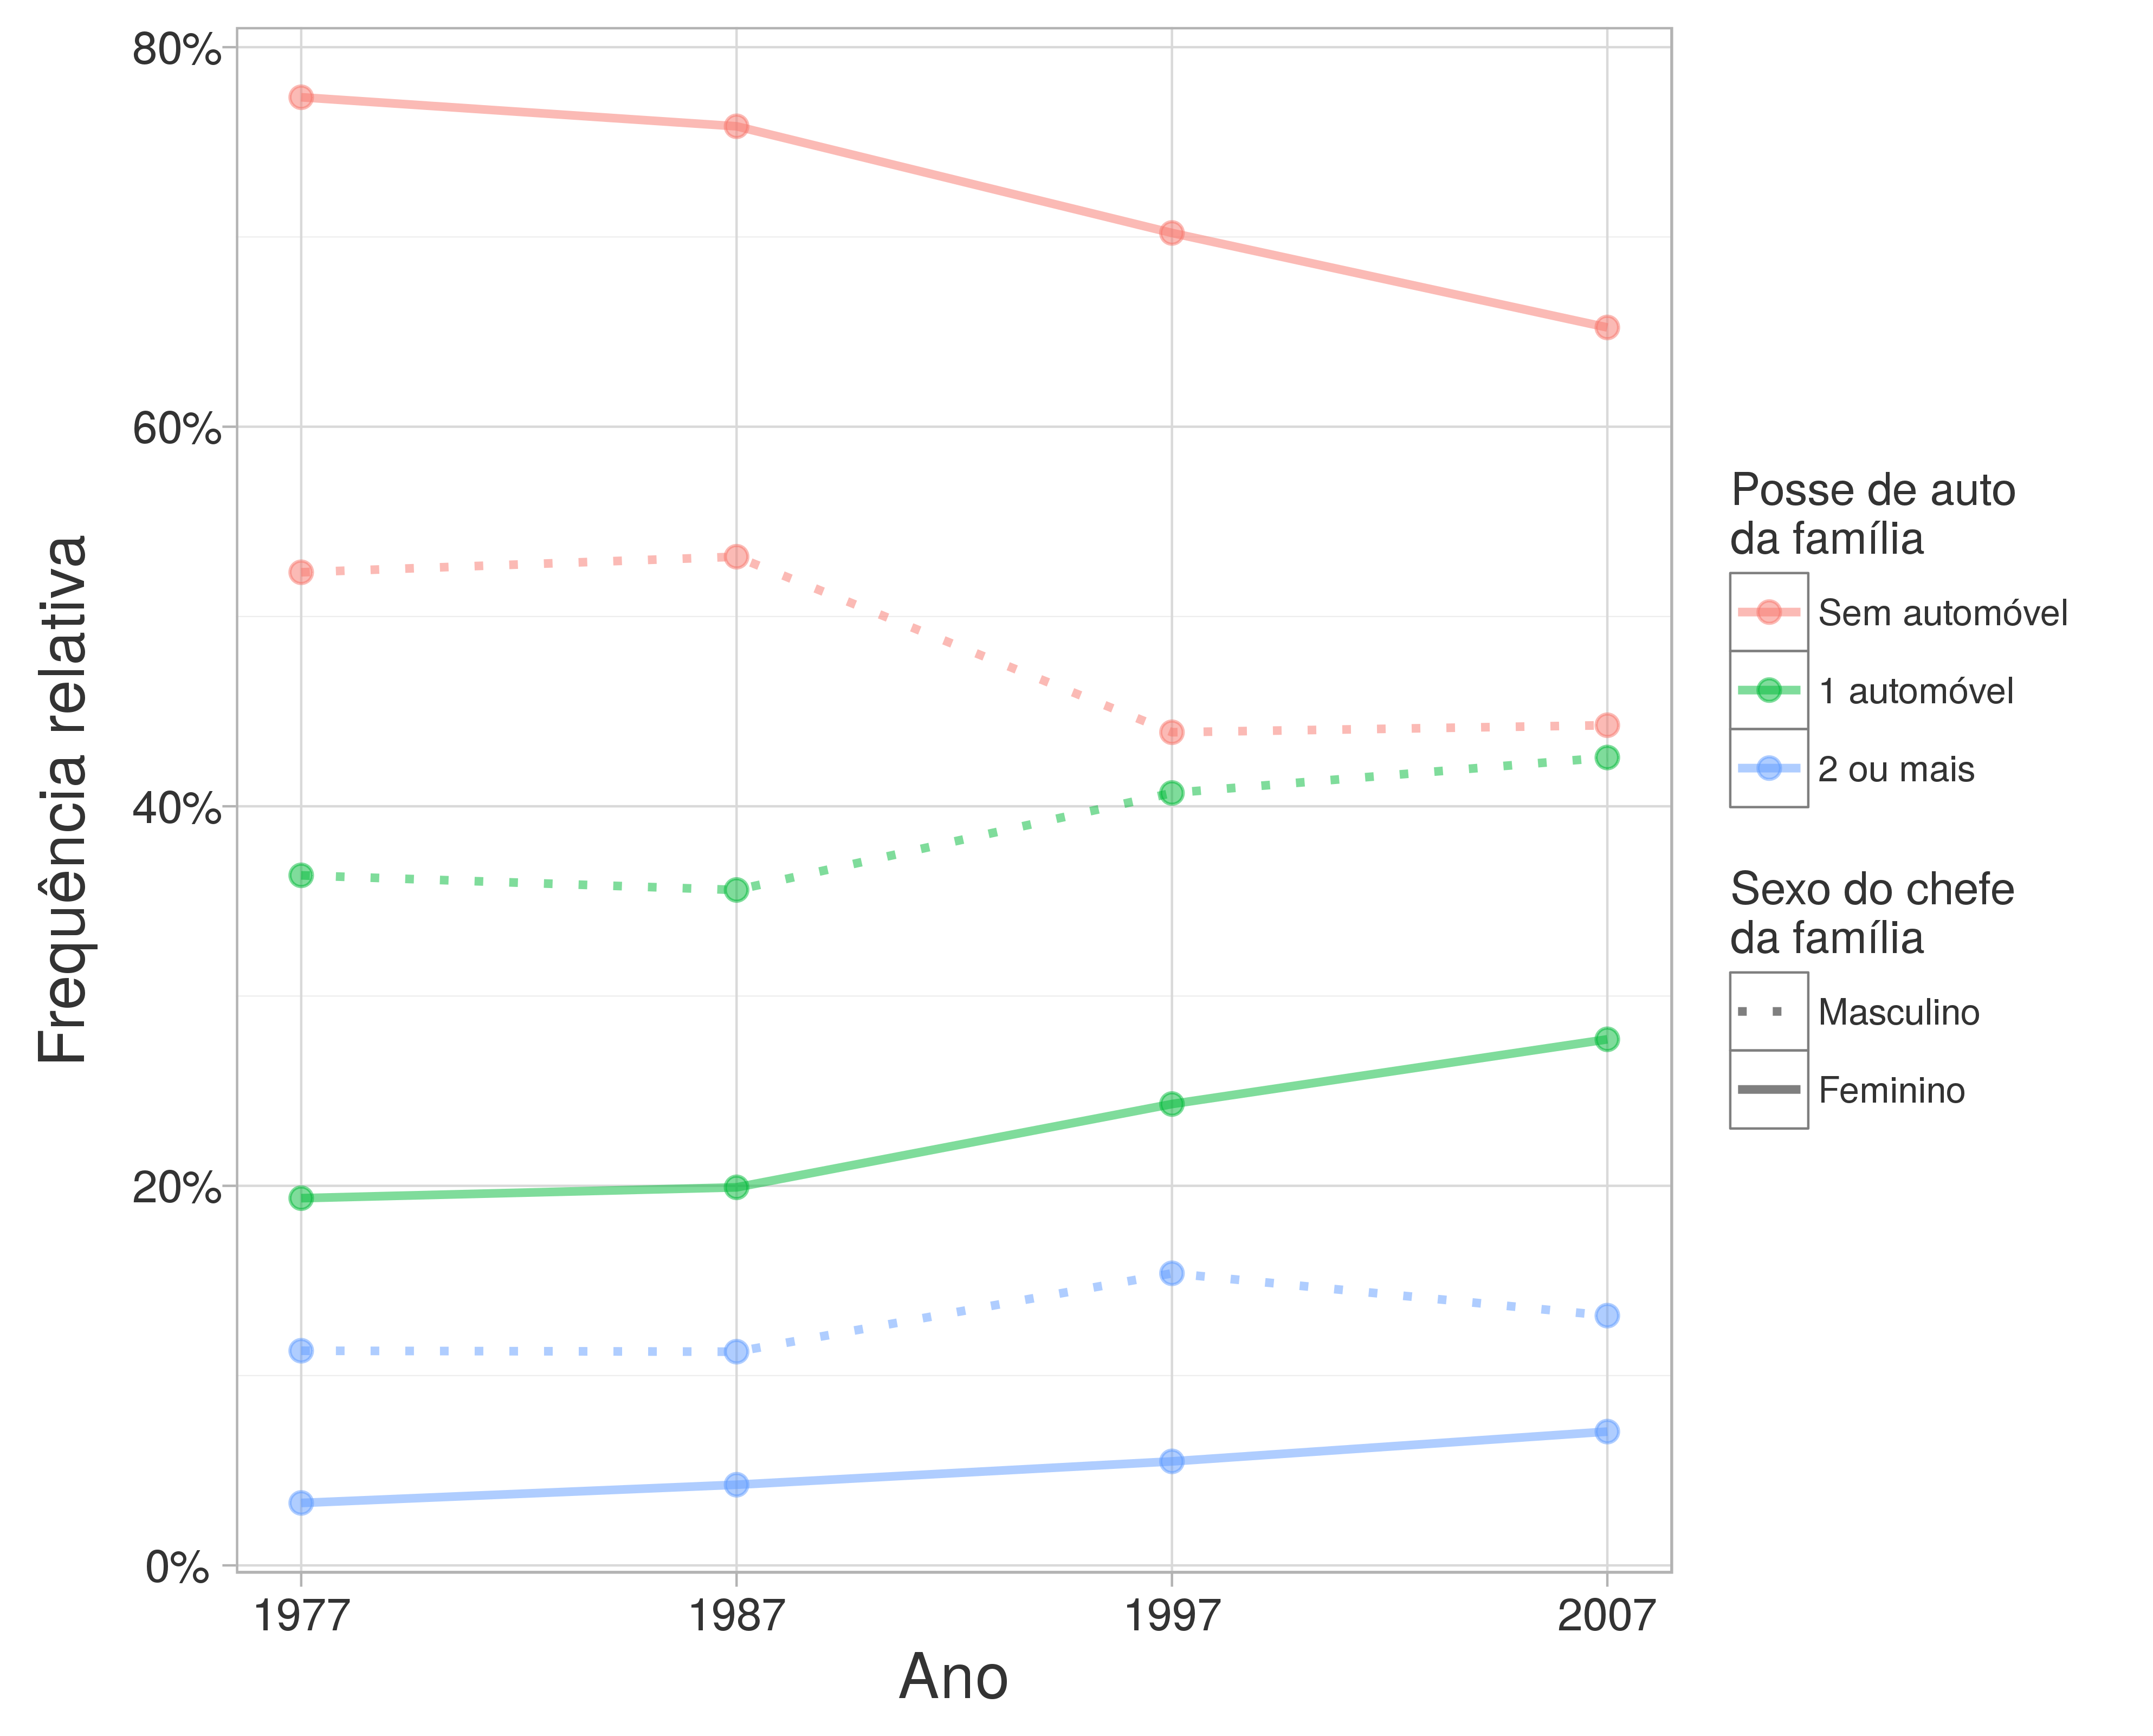
\includegraphics[width=1\textwidth]{./imagens/autos-sit-fam-sexo.png}%
    \end{center}%
    %\fonte{Compilação própria}
\end{grafico}%


A quantidade de motocicletas (\textbf{QT_MOTO}) e bicicletas (\textbf{QT_BICI}) foram levantadas apenas na Pesquisa OD de 2007, e tem suas estatísticas descritivas são apresentadas na Tabela \ref{tab:estat-qt-moto-bici}.
Percebe-se que, embora um meio de transporte individual motorizado mais barato, a incidência da posse de motocicletas é uma fenômeno mais raro, provavelmente devido ao risco associado a esse meio de transporte
\footnote{Segundo dados da CET o índice de acidentes com motociclistas...}. 
%TODO preencher nota de rodapé

Essa falta de segurança na condução do meio de transporte também ocorre com a bicicleta, porém, além de ser ainda mais barata que a motocicleta, ela não é motorizada e, por isso, comumente trafega nos passeios públicos e calçadas, onde o(a) condutor(a) sofre menor risco de colisão com meios motorizados de transporte (motocicletas, carros, ônibus e caminhões). Com a recente política municipal de incentivo à bicicleta como meio de transporte, por meio de investimentos em infraestrutura cicloviária, é possível que na Pesquisa OD de 2017 haja evoluções destes dados que mereçam investigação.
Vale lembrar que existe também a questão do status associado muito mais fortemente à posse do automóvel do que da motocicleta; e no caso das bicicletas, seu uso é associado à ideia de pobreza e falta de recursos suficientes para comprar um carro.
%TODO por referências aqui

\begin{table}[htb]
\centering
   \IBGEtab{%\renewcommand{\arraystretch}{1.5}%%\ABNTEXfontereduzida%
        \renewcommand{\arraystretch}{1.5}
        \caption{Estatísticas das variáveis ``QT_MOTO'' e ``QT_BICI''}
        \label{tab:estat-qt-moto-bici}
    }{%

    \begin{tabular}{cccccc}
        \toprule
        \textbf{2007} & \textbf{Mínimo} & \textbf{1º Quartil} & \textbf{Mediana} & \textbf{3º Quartil} & \textbf{Máximo}  \\ \midrule \midrule
        \textbf{motocicleta}  &  0 &  0 &  0 &  0 &  9 \\ \hline
        \textbf{bicicleta} &  0 &  0 &  0 &  1 &  9 \\ \bottomrule
        \textbf{ANO} & \textbf{Média} & \textbf{Desvio Padrão} & \textbf{Assimetria} & \textbf{Curtose} & \textbf{Nº de ``NA''}  \\ \midrule \midrule
        \textbf{motocicleta}  & 0,07 & 0,29 & 5,86 & 74,31 &      0 \\ \hline
        \textbf{bicicleta} & 0,46 & 0,8 & 2,27 & 7,5 & 0 \\ \bottomrule
        \end{tabular}
    }

\end{table}
% Estatísticas para registros com F_FAM==1

A variável \textbf{TOT_PESS}, um dado de contagem, indica quantas pessoas existem na família e tem suas estatísticas descritivas apresentadas na Tabela \ref{tab:estat-tot-pess}. Não haviam \textit{missing values} e o valor médio indica que o tamanho da família diminuiu, passando de pouco mais de 4 pessoas em 1977 para pouco menos de 3 pessoas por família em 2007.
Em comportamento análogo a TOT_FAM, a Figura \ref{fig:box-plot-tot-pess} indica que a influência dos \textit{outliers} de TOT_PESS diminui com o tempo, o que também se reflete na queda dos desvios padrão, que indica menor dispersão dos dados.

\begin{table}[htb]
\centering
   \IBGEtab{%\renewcommand{\arraystretch}{1.5}%%\ABNTEXfontereduzida%
        \renewcommand{\arraystretch}{1.5}
        \caption{Estatísticas da variável ``TOT_PESS''}
        \label{tab:estat-tot-pess}
    }{%

    \begin{tabular}{cccccc}
        \toprule
        \textbf{ANO} & \textbf{Média} & \textbf{Desvio Padrão} & \textbf{Assimetria} & \textbf{Curtose} & \textbf{Máximo}  \\ \midrule \midrule
        \textbf{1977}  & 4,13 & 2,09 & 0,99 & 1,78 & 18 \\ \hline
        \textbf{1987}  & 3,93 & 1,80 & 0,92 & 2,03 & 22 \\ \hline
        \textbf{1997}  & 3,68 & 1,73 & 0,82 & 1,68 & 17 \\ \hline
        \textbf{2007}  & 2,96 & 1,46 & 0,78 & 1,00 & 14 \\ \hline
        \textbf{Geral} & 3,65 & 1,83 & 1,00 & 2,10 & 22 \\ \bottomrule
        \end{tabular}
    }

\end{table}
% Estatísticas para registros com F_FAM==1


\begin{figure}[htb]%
    \caption{\label{fig:box-plot-tot-pess}Box plot da variável ``TOT_PESS'', por ano}%
    \begin{center}%
        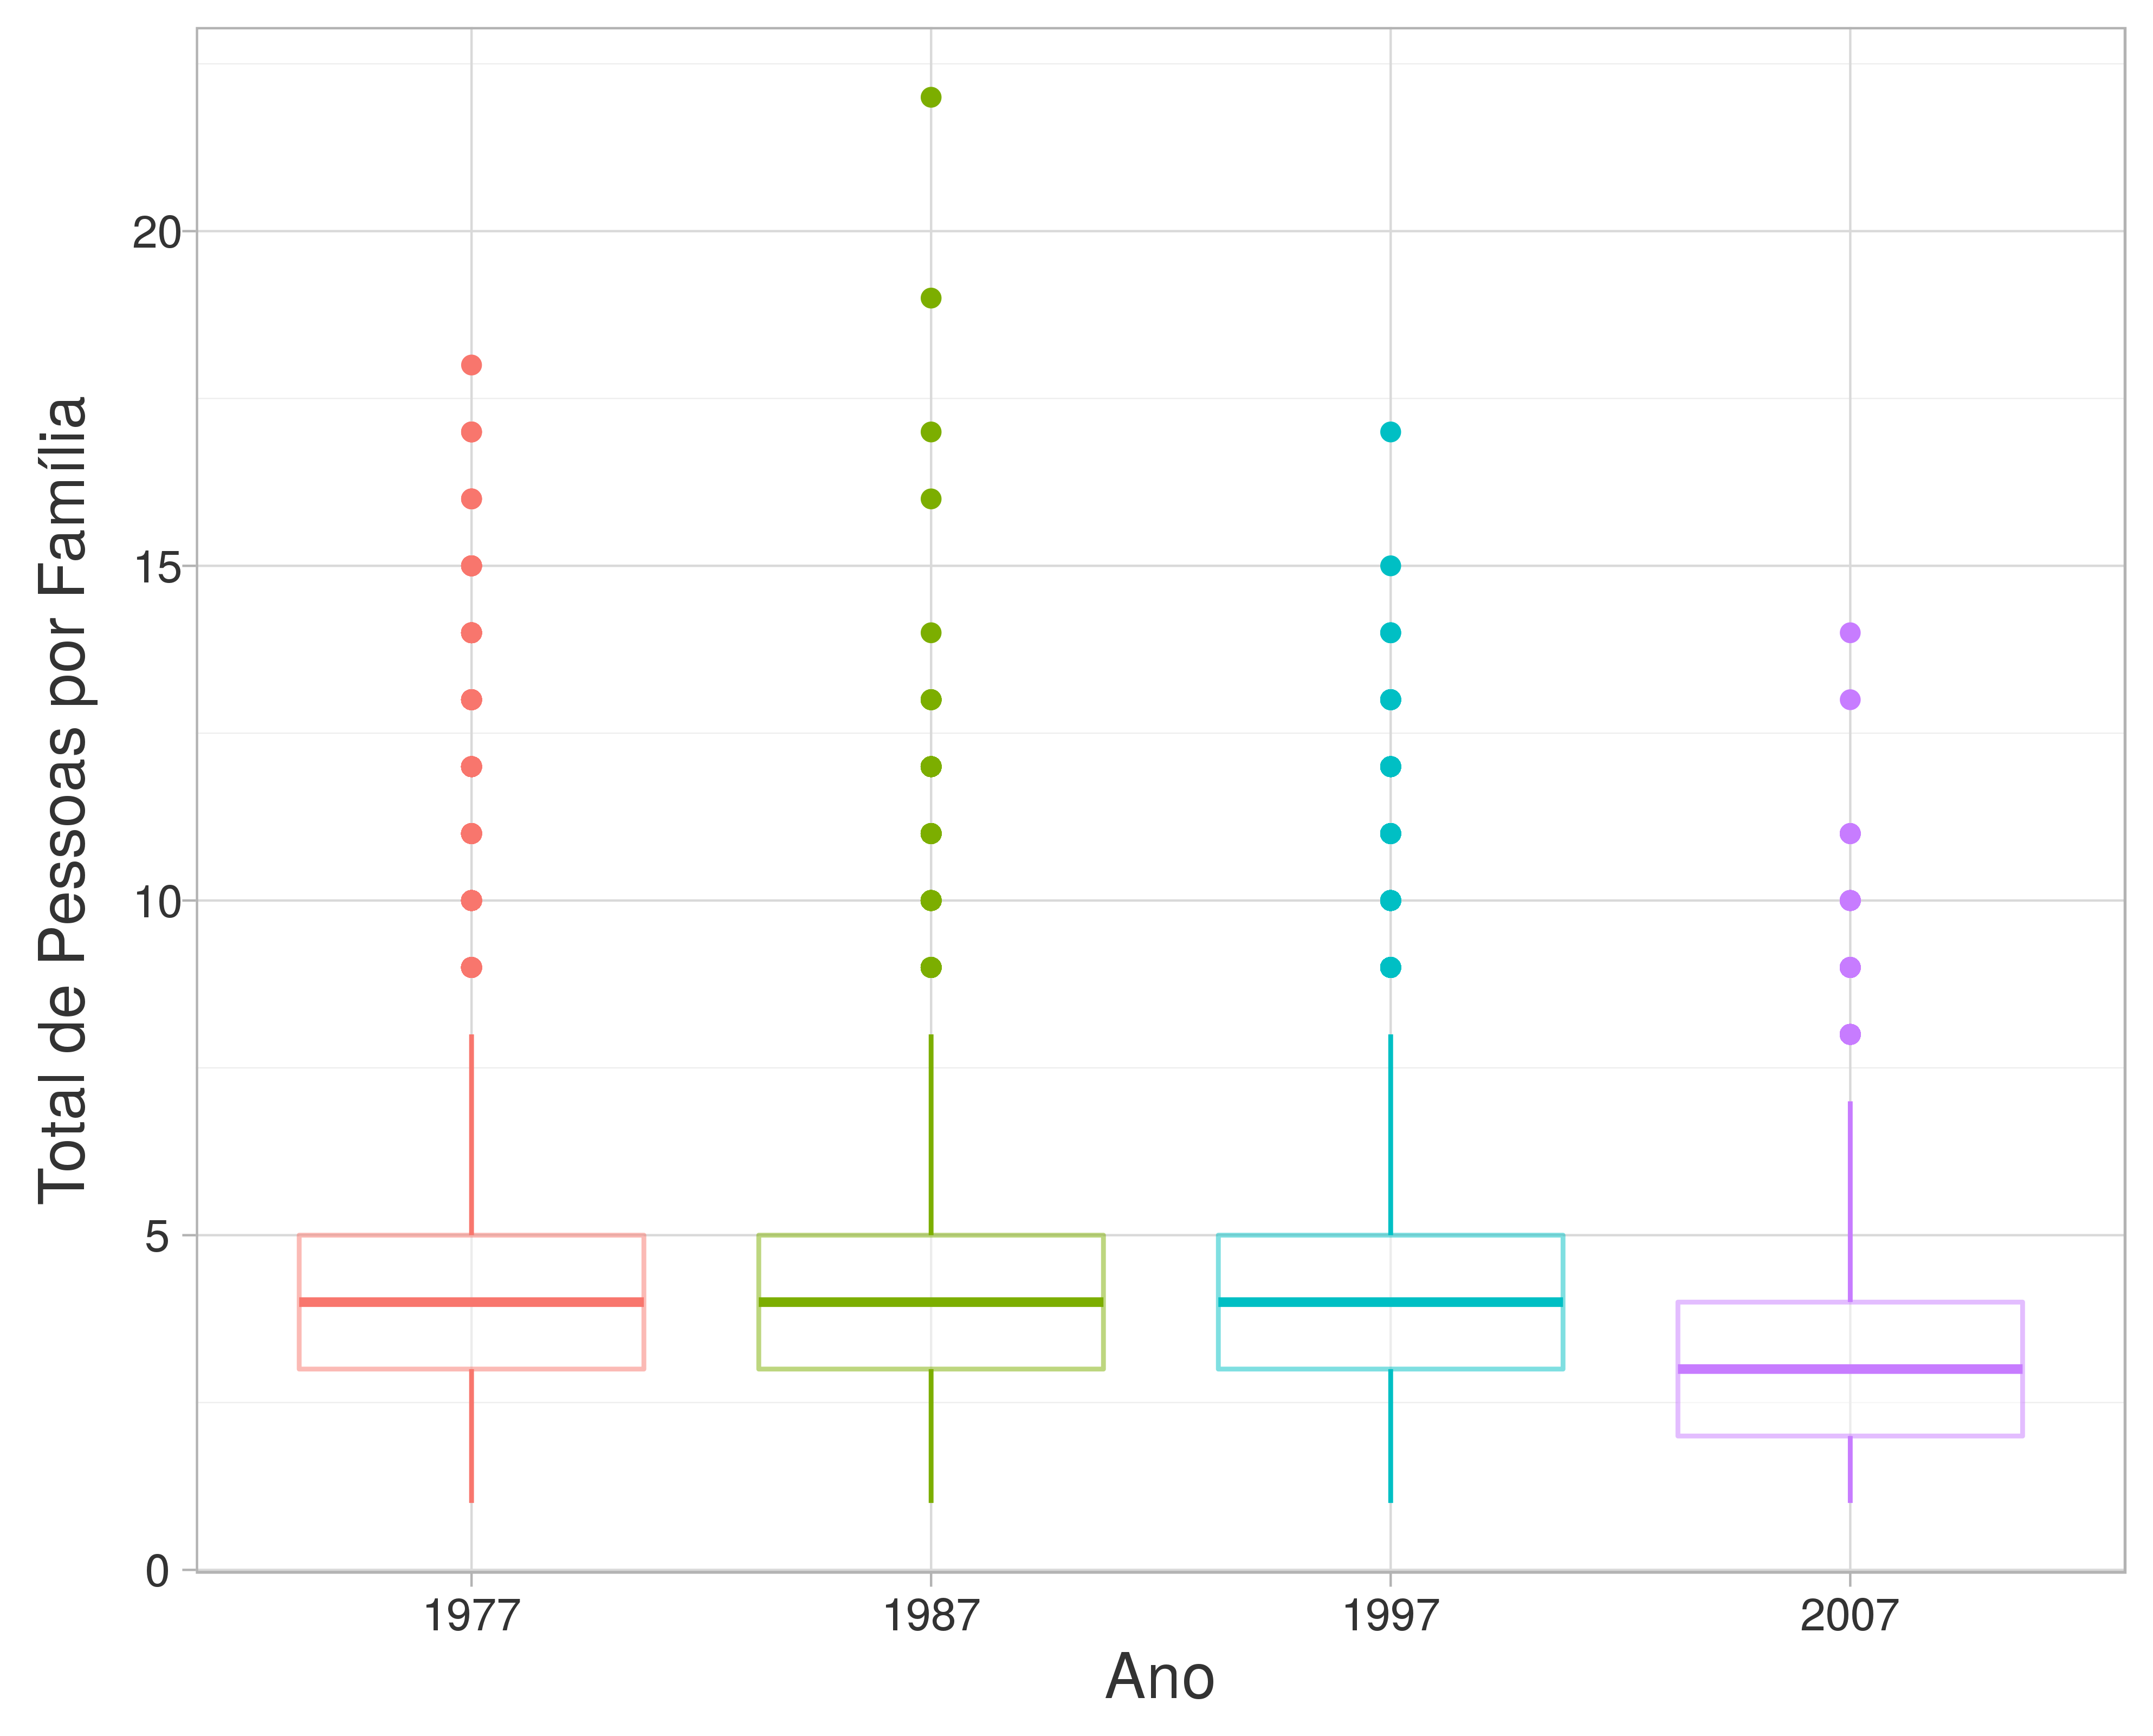
\includegraphics[width=1\textwidth]{./imagens/box-plot-tot-pess.png}%
    \end{center}%
    %\fonte{Compilação própria}
\end{figure}%

Percebe-se pelo Gráfico \ref{graf:pres-flh-idoso-fam} a tendência de diminuição geral nas porcentagens de famílias com filhos pequenos (até 9 anos) a partir de 1987, efeito que será percebido na faixa etária seguinte (entre 10 e 19 anos) em 1997. Essa diminuição da presença de dependentes jovens (crianças/adolescentes) mantém-se em 2007. Nos mesmos períodos de análise, ocorre o envelhecimento da população, efeito capturado no gráfico pela presença de idosos (acima de 60 ou de 70 anos) com taxas positivas de crescimento.

\begin{grafico}[htb]%
    \caption{\label{graf:pres-flh-idoso-fam}Proporção de famílias com presença de dependentes, por ano}%
    \begin{center}%
        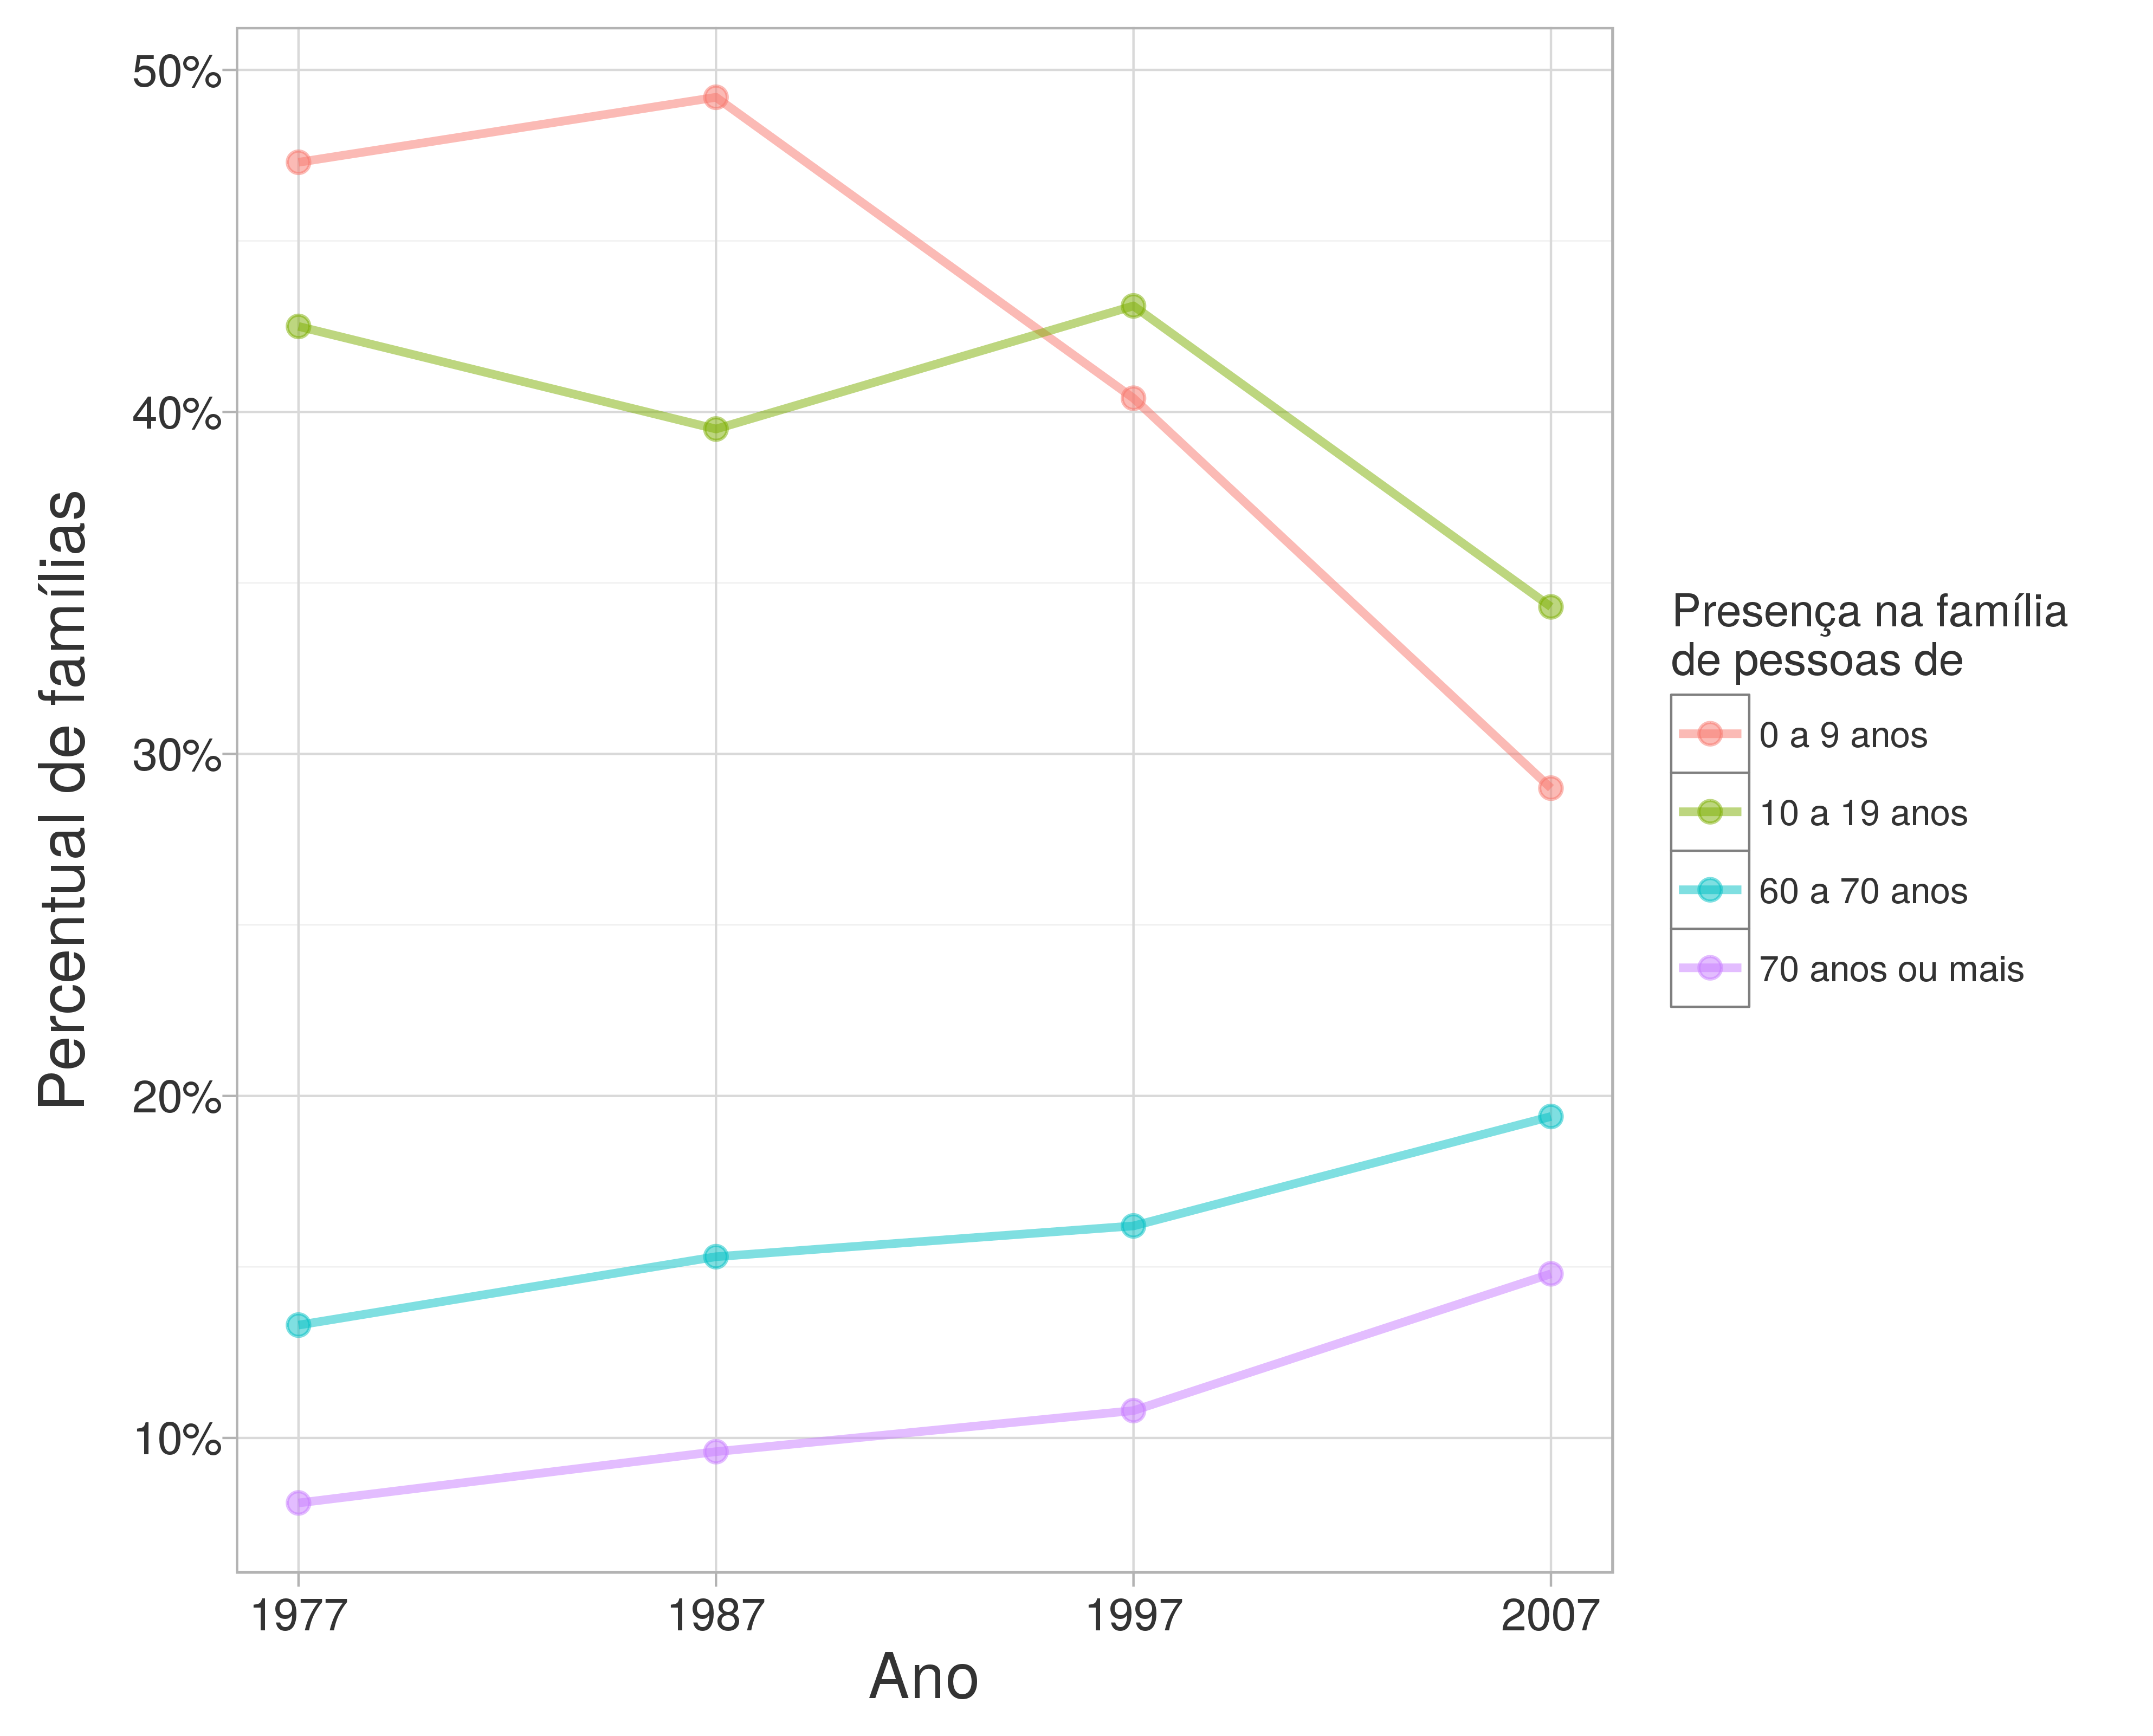
\includegraphics[width=1\textwidth]{./imagens/pres-flh-idoso-fam.png}%
    \end{center}%
    %\fonte{Compilação própria}
\end{grafico}%

Como um dos fatores do indivíduo que influencia seu padrão de deslocamentos está o estágio no ``ciclo de vida'' \cite{BILT1997}.
Isto é, as atividades desenvolvidas por uma pessoa depende em que fase da vida ela, e também os demais membros da família, se encontram. A variável \textbf{IDADE} é uma das variáveis que definem o ciclo de vida das pessoas. É possível perceber no Gráfico \ref{graf:distr-idade} que houve uma transição da pirâmide etária da RMSP, indicando envelhecimento da população tanto masculina como feminina.

\begin{grafico}[htb]%
    \caption{\label{graf:distr-idade}Distribuição da variável ``IDADE'' de respondentes, por ano e por sexo}%
    \begin{center}%
        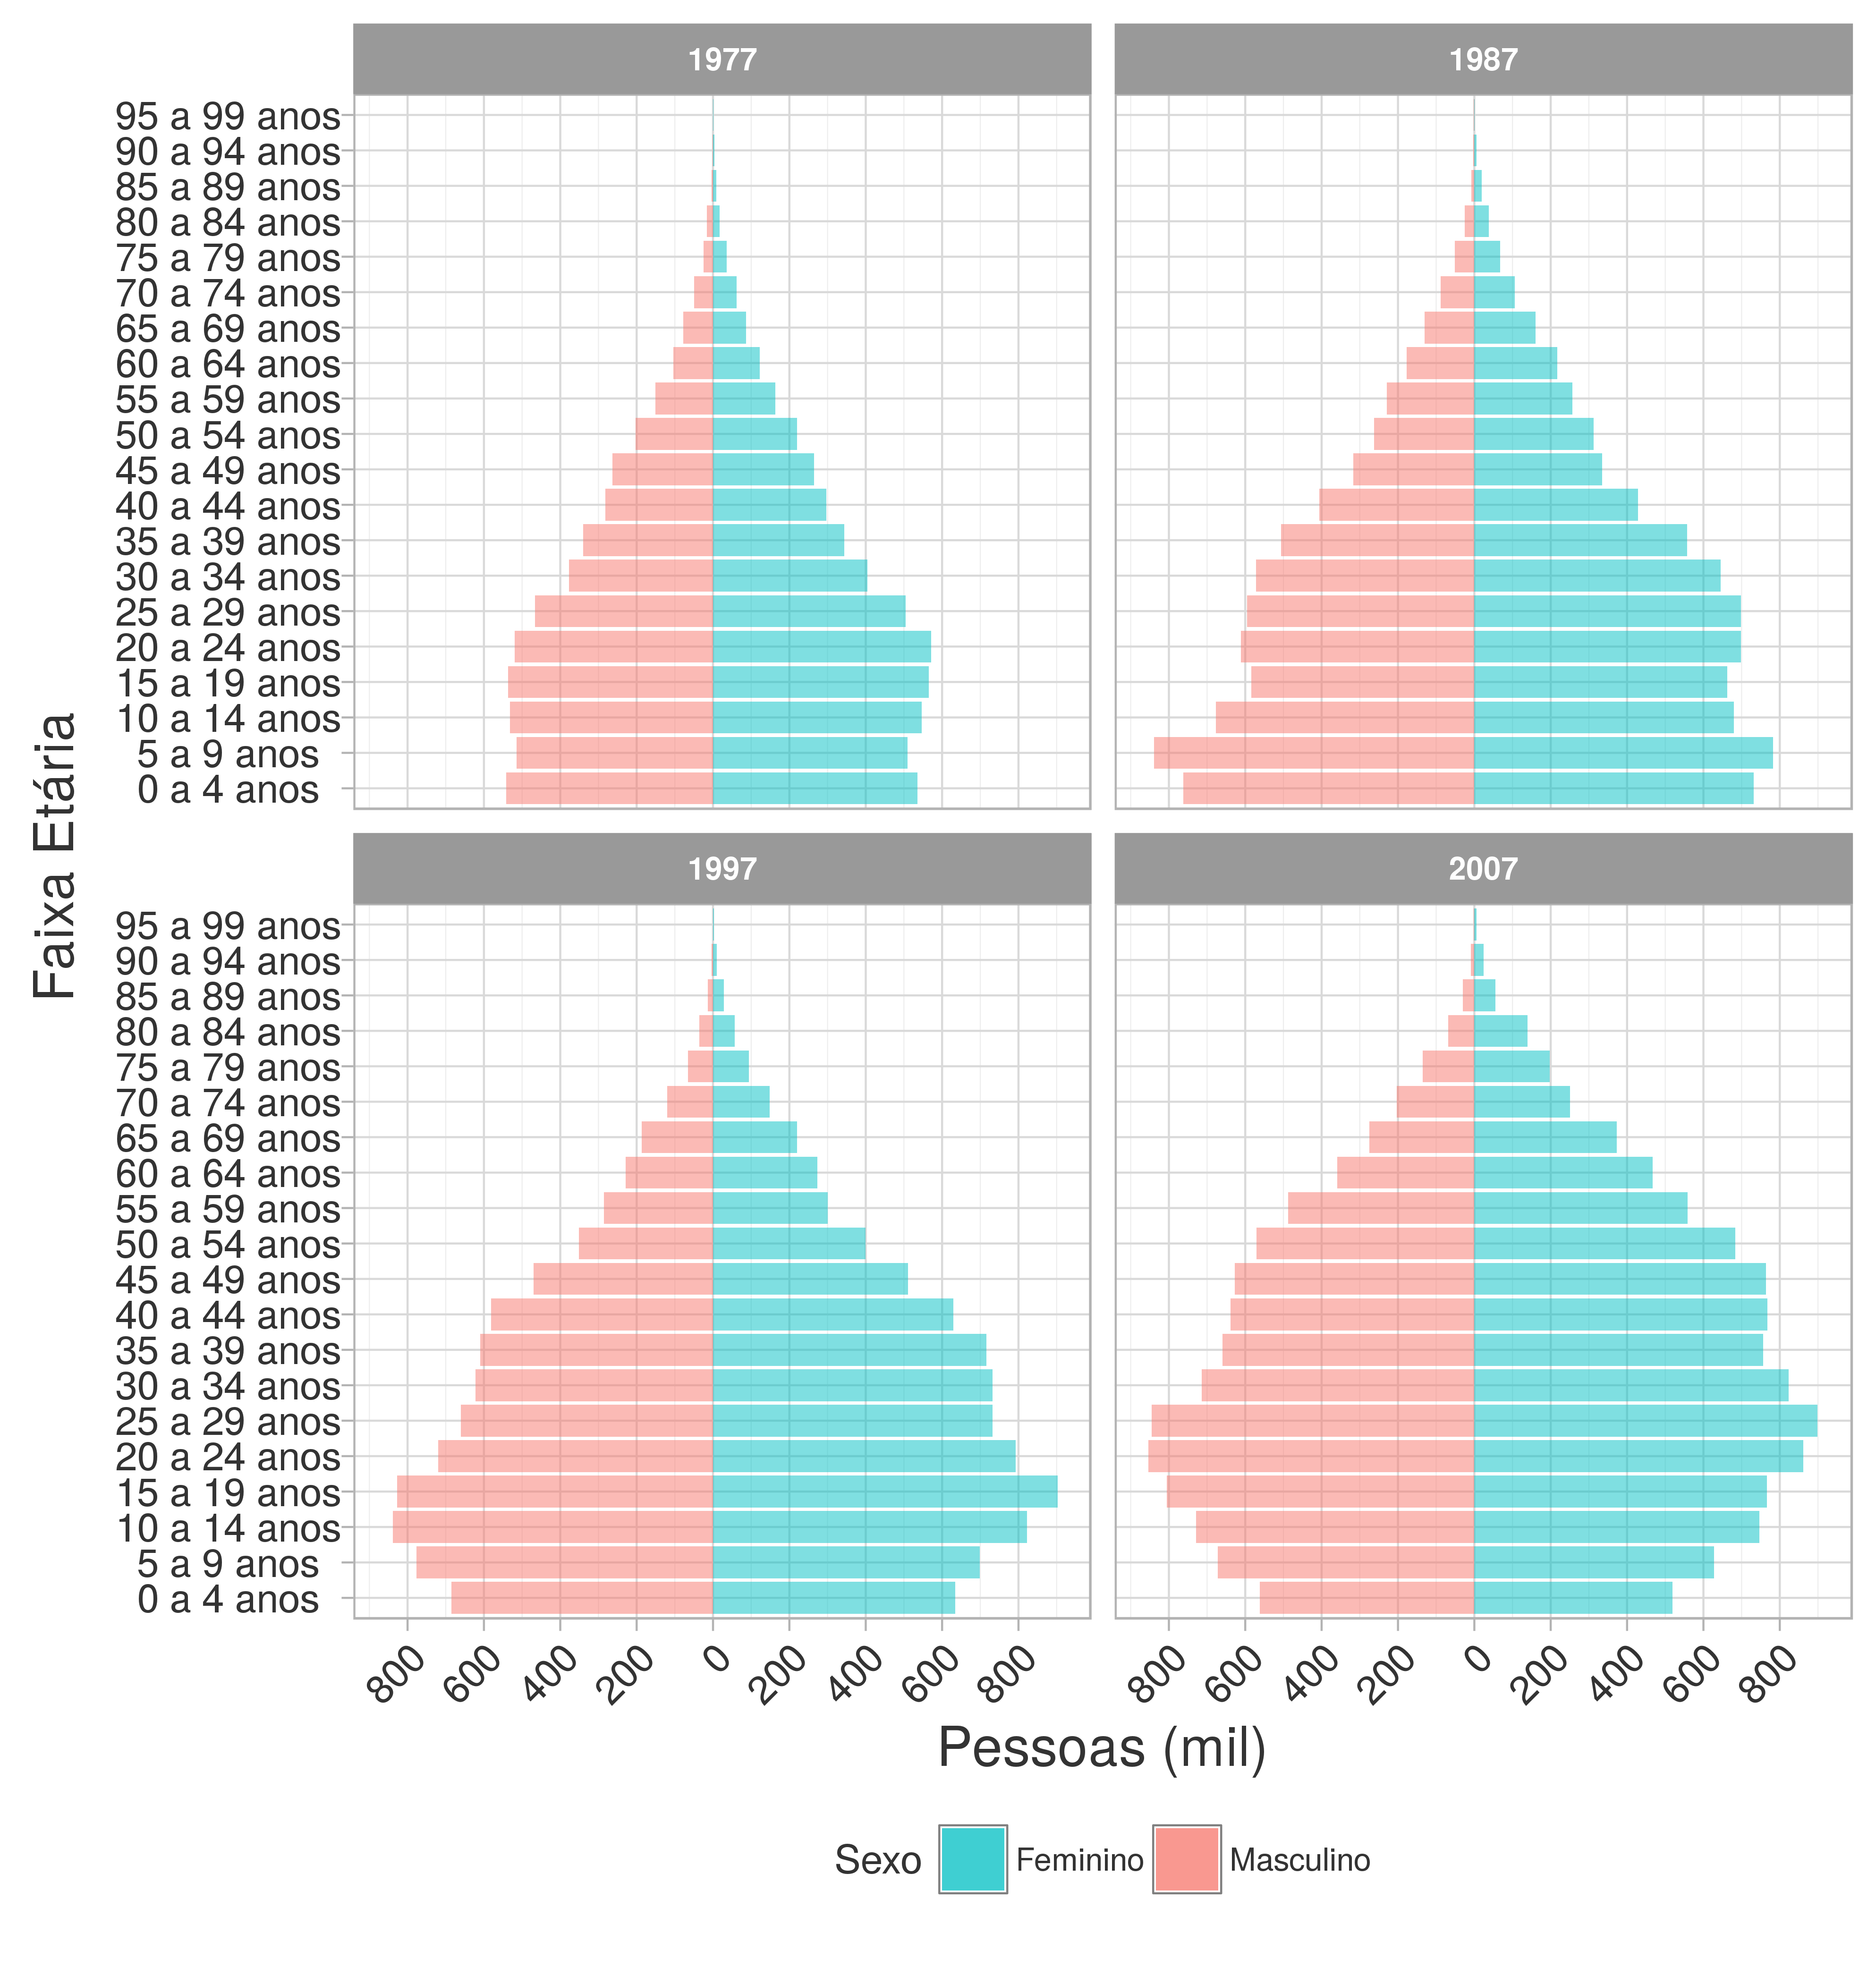
\includegraphics[width=1\textwidth]{./imagens/idade.png}%
    \end{center}%
%    \fonte{Compilação própria}
\end{grafico}%

Embora não exista relação identitária entre sexo e gênero, conforme já exposto na revisão de literatura, a variável \textbf{SEXO} é uma componente importante para compreender a categoria de análise gênero. Percebe-se na Tabela \ref{tab:prop-sexo} que em todos os anos a proporção de mulheres entrevistadas é superior à de homens, provavelmente devido ao fato de a pesquisa ser domiciliar e ser mais provável encontrar mulheres do que homens em casa.

\begin{table}[htb]
    \IBGEtab{%\renewcommand{\arraystretch}{1.5}%%\ABNTEXfontereduzida%
        \renewcommand{\arraystretch}{1.5}
        \caption{Frequências absoluta e relativa da variável SEXO, por ano}
        \label{tab:prop-sexo}
    }{%

    \begin{tabular}{ccccc}
        \toprule
        \textbf{ANO} & \textbf{1977} & \textbf{1987} & \textbf{1997} & \textbf{2007}\\ \midrule \midrule
        \textbf{\ quantidade de pessoas do sexo masculino na amostra} & 52.162 & 53.176 & 47.326 & 42.289 \\ \midrule
        \textbf{\% de pessoas do sexo masculino} & 48,3 & 48,0 & 47,9 & 46,3  \\ \midrule
%        \textbf{\% de pessoas do sexo masculino expandido} & 48,7 & 48,0 & 48,1 & 47,3  \\ \midrule        
        \textbf{\ quantidade de pessoas do sexo feminino na amostra} & 55.866 & 57.637 & 51.454 & 49.116  \\ \midrule
        \textbf{\% de pessoas do sexo feminino}  & 51,7 & 52,0 & 52,1 & 53,7  \\ \bottomrule
%        \textbf{\% de pessoas do sexo feminino expandido}  & 51,3 & 52,0 & 51,9 & 52,7 \\ \bottomrule
        \end{tabular}
    }

\end{table}
% Estatísticas para registros com F_PESS==1

Observando a variável situação familiar (\textbf{SIT_FAM}), nota-se que para as mulheres houve uma mudança ao longo dessas três décadas - ver Gráfico \ref{graf:distr-sit-fam}. Em 1977, era mais frequente elas ocuparem a posição de filhas (41,8\%), em seguida de cônjuges (36,3\%). A posição de ``pessoa responsável'' pela família é a quarta categoria mais frequente (6,3\%), de seis. Tal distribuição permanece semelhante em 1987. Em 1997, no entanto, a posição de ``pessoa responsável'' pela família (11,1\%) já quase se equipara à posição de ``outro parente/agregado(a)'' (11,3\%). Em 2007, se aproxima de um quarto proporção das mulheres entrevistadas que são responsáveis por suas famílias (22,6\%), representando aumento demais de 3,5 vezes em relação aos percentuais de 1977. O percentual de mulheres cônjuges/companheiras pouco se altera ao longo do tempo, permanecendo na faixa dos 35\%. Há diminuição da posição de empregado(a) doméstico(a) para as mulheres (da ordem da metade). Existe, também, queda da frequência daqueles que se declaram na posição de filho(a) ou enteado(a) tanto para homens como para mulheres - em ordem de grandeza próxima: cerca de 10\% para mulheres e 9\% para homens. Isso pode ser reflexo da diminuição das taxas de fecundidade%
\footnote{Por ``taxa de fecundidade total'' entende-se o número médio de filhos que teria uma mulher de uma coorte hipotética (15 e 49 anos de idade) ao final de seu período reprodutivo. Fonte: IBGE. Disponível em: \url{http://www.ibge.gov.br/home/estatistica/populacao/condicaodevida/indicadoresminimos/conceitos.shtm\#tf}} 
da população (ver Tabela \ref{tab:taxa-fecund}). Entre os homens percebe-se que houve crescimento entre aqueles com posição de ``pessoas responsável'' de cerca de 3,5\%, e também dos que declaram-se cônjuge/companheiro (cerca de 20 vezes) - esta última constatação é coerente com o fato de mais mulheres serem a principal fonte de renda doméstica, ou seja, a ``pessoa responsável'' da família.

\begin{table}[htb]
    \IBGEtab{%\renewcommand{\arraystretch}{1.5}%%\ABNTEXfontereduzida%
	    \renewcommand{\arraystretch}{1.5}
        \caption{Evolução das taxas de fecundidade no Brasil, de 1970 a 2010}
		\label{tab:taxa-fecund}
    }{%
	    \begin{tabular}{P{5.00cm} P{1.50cm} P{1.50cm} P{1.50cm} P{1.50cm} P{1.50cm}}
            \toprule
	           \headerTabCenterCell{Ano} &
   	           \headerTabCenterCell{1970} &
   	           \headerTabCenterCell{1980} &
   	           \headerTabCenterCell{1991} &
   	           \headerTabCenterCell{2000} &
   	           \headerTabCenterCell{2010} \\
		    \midrule \midrule
				Taxa de fecundidade (Brasil)&
				5,8&
				4,4&
				2,7&
				2,4&
		        1,9\\
			\midrule
				Taxa de fecundidade (Sudeste)&
				4,6&
				3,2&
				2,4&
				2,1&
		        1,7\\
			\midrule
				Taxa de fecundidade (São Paulo)&
				3,94&
				3,24&
				2,28&
				2,05&
		        1,67\\
			\bottomrule	
		\end{tabular}
    }{%
		\fonte{Compilação a partir de dados dos censos do IBGE disponíveis em \url{http://seculoxx.ibge.gov.br/populacionais-sociais-politicas-e-culturais/busca-por-palavra-chave/populacao/810-fecundidade} Acesso em 17 de novembro de 2014}
		\nota{Ao analisar as taxas de fecundidades para as Grandes Regiões, nota-se que o Sudeste tem os menores percentuais de mulheres que tiveram filhos em todos os subgrupos etários.}
		}
\end{table}

Tem-se como uma das hipótese deste trabalho que houve evolução dos padrões de mobilidade por gênero.
Articular as variáveis sexo e situação familiar é uma melhor estratégia para tentar utilizar o gênero como categoria de análise.
Assim, a transformação dos papeis sociais desempenhados por homens e mulheres dentro do núcleo familiar ao longo das últimas décadas pode ter alterado de maneira significativa os respectivos padrões de mobilidade.

\begin{grafico}[htb]%
    \caption{\label{graf:distr-sit-fam}Distribuição da variável ``SIT_FAM'', por ano e por sexo}%
    \begin{center}%
        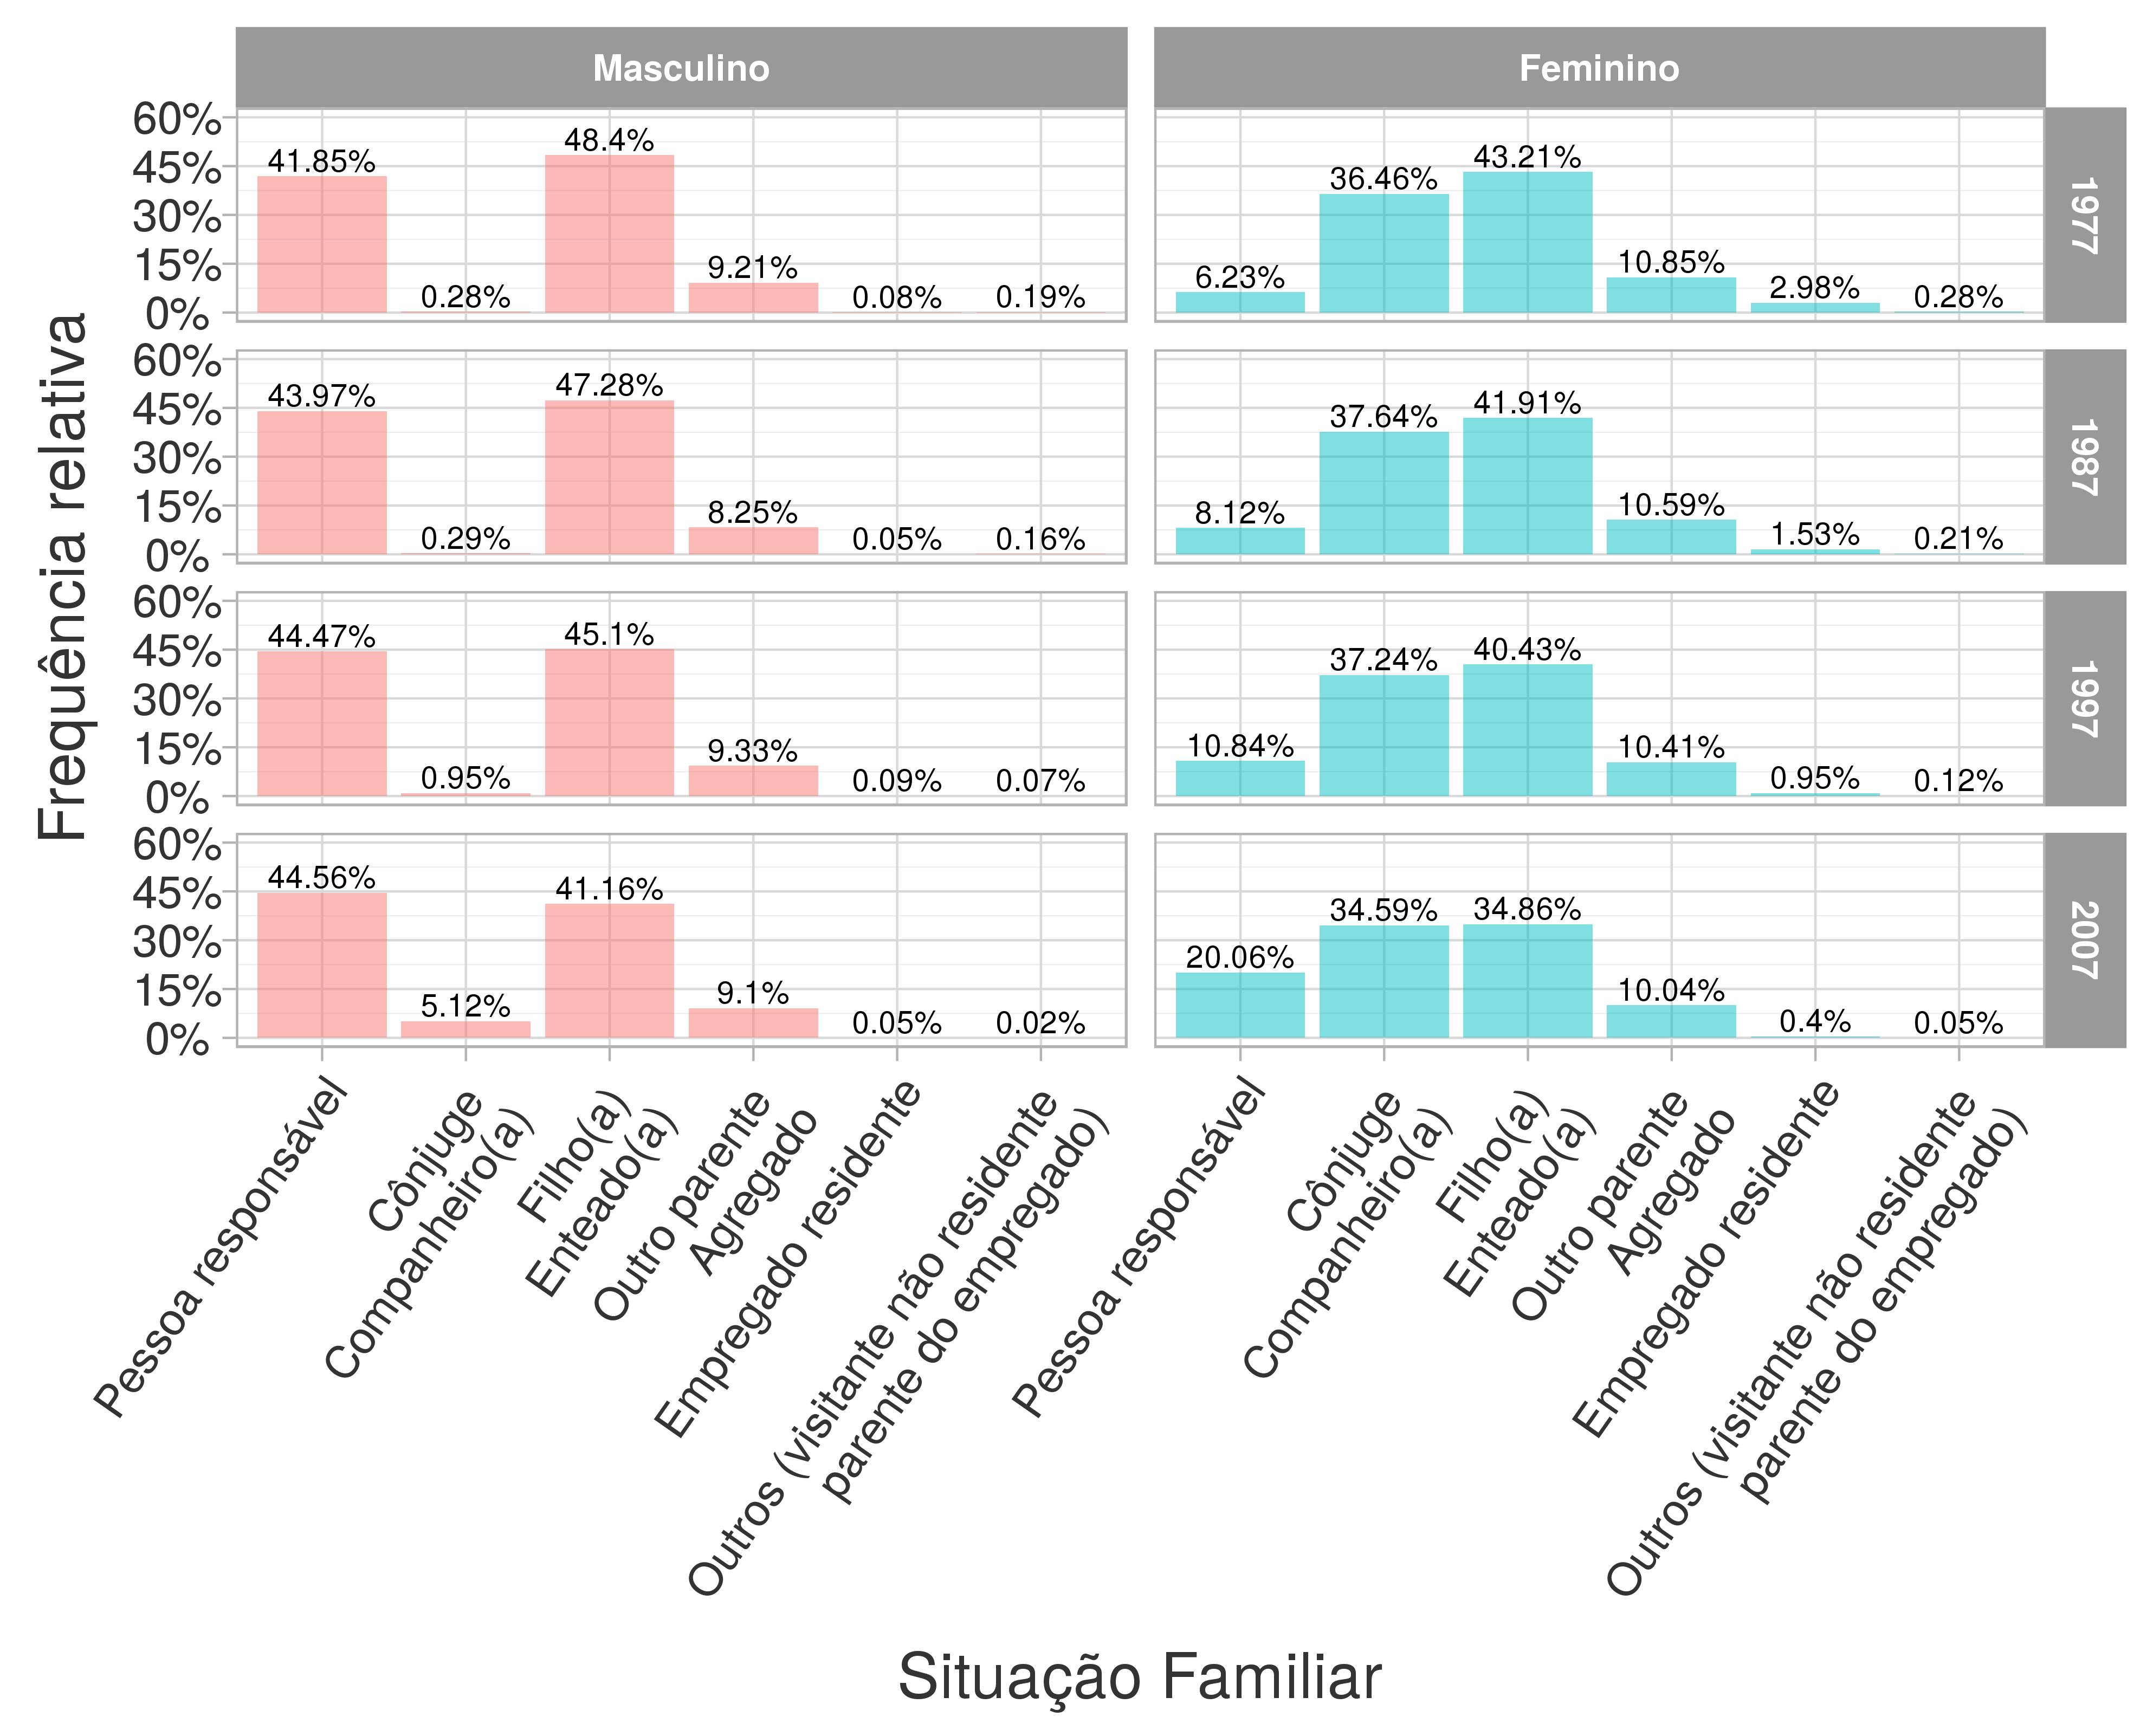
\includegraphics[width=1\textwidth]{./imagens/sit-fam.png}%
    \end{center}%
%    \fonte{Compilação própria}
\end{grafico}%

\citeauthoronline{BILT1997} (\citeyear{BILT1997}), a partir da análise de trabalhos de diversos autores, para compreender melhor o comportamento das pessoas em relação à participação em atividades e a consequente geração de viagens, 
elenca como conceito importante, além do estágio no ciclo de vida familiar e dos papéis sociais, o estilo de vida.
Duas das variáveis que auxiliam a caracterizar o estilo de vida da pessoa respondente é saber se ela estuda e se ela trabalha.

A variável \textbf{TRABALHA} foi construída a partir da variável OCUP da seguinte maneira: se a categoria da ocupação fosse 1, correspondente a ``tem trabalho'', a variável recebia valor 1, caso contrário, recebia valor 0.
A variável \textbf{ESTUDA} conta com as categorias sim (1) e não (0). Em 1987, 1997 e 2007 esta variável existe, mas somente com a categoria ``não'' em comum. Assim, as demais alternativas de resposta tornaram-se simplesmente ``sim'', independente das subdivisões que apresentassem. Para 1977, ano em que essa variável não existe, ela foi preenchida segundo o seguinte critério: a pessoa foi considerada estudante se o campo ``Zona da escola'' dela não fosse vazio ou igual a zero. Preferiu-se não utilizar a categoria ``estudante'' da variável ocupação para não perder a informação de quem estuda e trabalha, pois neste caso, estudante não seria a ocupação principal da pessoa e sim ``tem trabalho''.

% Fazendo o seguinte:
% od %>% filter(SERV_PAS_DEST==1, ZONA_DEST==ZONA_ESC, SUBZONA_DEST==SUBZONA_ESC, ANO==1) %>% select(ESTUDA, ID_PESS) %>% count(ID_PESS)
% Obtive: 72 pessoas que podem ter sido registrados erroneamnte domo estudantes em 1977

As Tabelas \ref{tab:prop-estuda} e \ref{tab:prop-trabalha} indicam as frequências das \textit{dummies} TRABALHA e ESTUDA, por ano e por sexo, em relação à população (aplicados os fatores de expansão).
Percebe-se que o percentual de trabalhadores(as) aumenta na população devido à maior participação feminina no mercado de trabalho, dado que os percentuais dos trabalhadores permanecem no mesmo patamar (24\% da população). Segmentando por sexo, vê-se que houve um aumento de quase 20\% na participação feminina no mercado de trabalho e pouco mais de 2\% de incremento na masculina.
Analisando as proporções de mulheres e homens estudantes, nota-que que houve pequeno crescimento entre 1977 e 1997 (3,2\% feminino e 2,5\% masculino) seguido de leve queda (1,5\% pra ambos sexos). A expectativa era de ter havido um grande crescimento percentual do número de estudantes, especialmente mulheres, para o período observado. O crescimento tímido pode dever-se ao fato de que, embora a população da RMSP tenha elevado seus níveis de escolarização, o crescimento (desacelerando) e o envelhecimento (em ascensão) da população implicam haver mais gente fora da faixa etária escolar do que dentro dela. As quedas no percentual de estudantes pode estar relacionada tanto ao envelhecimento da população quanto à saturação do sistema de ensino, cuja obrigatoriedade de oferta pública limita-se à Educação Básica (9 anos de Ensino Fundamental e 3 anos de Ensino Médio). 


\begin{table}[htb]
    \IBGEtab{%\renewcommand{\arraystretch}{1.5}%%\ABNTEXfontereduzida%
        \renewcommand{\arraystretch}{1.5}
        \caption{Frequências da variável TRABALHA, por ano e sexo}
        \label{tab:prop-trabalha}
    }{%

    \begin{tabular}{ccccc}
        \toprule
        \textbf{ANO} & \textbf{1977} & \textbf{1987} & \textbf{1997} & \textbf{2007}\\ \midrule \midrule
        \textbf{\% de trabalhadoras relativo ao total da população} & 9,78 & 12,18 & 16,27 & 19,88  \\ \midrule
        \textbf{\% de trabalhadores relativo ao total da população} & 24,42 & 24,73 & 24,61 & 24,82  \\ \midrule
        \textbf{\% de trabalhadoras relativo ao total de mulheres} & 19,08 & 23,44 & 31,38 & 37,76  \\ \midrule
        \textbf{\% de trabalhadores relativo ao total de homens} & 50,12 & 51,50 & 51,13 & 52,42  \\ \midrule
        \textbf{\% de trabalhadores(as) relativo ao total da população} & 34,20 & 36,91 & 40,89 & 44,70  \\ \bottomrule
        \end{tabular}
    }

\end{table}
% Estatísticas para registros com F_PESS==1

%No campo OCUP (35) as classificações de cada ano são bastante diferentes. Assim, decidiu-se por discriminar quem não respondeu, quem é estudante, quem é dono(a) de casa, que é aposentado(a), quem não tem ocupação (como por exemplo, crianças), quem está desempregado(a), quem está em licença e quem trabalha (em todas opções possíveis dadas em todas as Pesquisas OD).
%
%\begin{table}[htb]
%    \IBGEtab{%\renewcommand{\arraystretch}{1.5}%%\ABNTEXfontereduzida%
%        \renewcommand{\arraystretch}{1.5}
%        \caption{Estatísticas da variável ``OCUP''}
%        \label{tab:estat-ocup}
%    }{%
%
%    \begin{tabular}{cccccc}
%        \toprule
%        \textbf{ANO} & \textbf{1977} & \textbf{1987} & \textbf{1997} & \textbf{2007} & \textbf{Total}\\ \midrule \midrule
%        \textbf{OCUP=1}  &  3.666 & 41.082 & 41.474 & 43.838 & 163.060 \\ \hline
%        \textbf{OCUP=2}  &    736 &    668 &    447 &    574 &   2.425 \\ \hline
%        \textbf{OCUP=3}  &  3.869 &  6.664 &  7.553 & 13.125 &  31.211 \\ \hline
%        \textbf{OCUP=4}  &  2.256 &  3.304 &  6.297 &  6.500 &  18.357 \\ \hline
%        \textbf{OCUP=5}  & 16.519 & 17.118 &  8.604 &  6.717 &  48.958 \\ \hline
%        \textbf{OCUP=6}  & 22.571 & 20.283 & 11.484 &  7.082 &  61.420 \\ \hline
%        \textbf{OCUP=7}  & 20.415 & 21.409 & 22.921 & 13.569 &  78.314 \\ \hline
%        \textbf{OCUP=NA} &  4.996 &    285 &      0 &      0 &   5.281 \\ \bottomrule
%        \end{tabular}
%    }
%
%\end{table}
%% Estatísticas para registros com F_PESS==1
%
%No campo SETOR_ATIV (36), nos anos em que há opção de indicar o setor de mais de um trabalho (caso a pessoa tenha mais de um trabalho), foi considerado o setor do primeiro trabalho.
%
%\begin{table}[htb]
%    \IBGEtab{%\renewcommand{\arraystretch}{1.5}%%\ABNTEXfontereduzida%
%        \renewcommand{\arraystretch}{1.5}
%        \caption{Estatísticas da variável ``SETOR_ATIV''}
%        \label{tab:estat-setor-ativ}
%    }{%
%
%    \begin{tabular}{cccccc}
%        \toprule
%        \textbf{ANO} & \textbf{1977} & \textbf{1987} & \textbf{1997} & \textbf{2007} & \textbf{Total}\\ \midrule \midrule
%        \textbf{SETOR_ATIV=1}  &    252 &    252 &    394 &    163 &   1.061 \\ \hline
%        \textbf{SETOR_ATIV=2}  &  1.248 &  1.012 &  2.350 &  1.483 &   6.093 \\ \hline
%        \textbf{SETOR_ATIV=3}  & 12.381 & 12.391 &  6.002 &  4.676 &  35.450 \\ \hline
%        \textbf{SETOR_ATIV=4}  &  7.992 &  7.785 &  9.389 &  7.900 &  33.066 \\ \hline
%        \textbf{SETOR_ATIV=5}  &  3.336 &  3.745 &  1.693 &  1.544 &  10.318 \\ \hline
%        \textbf{SETOR_ATIV=6}  &    952 &  1.069 &  2.023 &  1.534 &   5.578 \\ \hline
%        \textbf{SETOR_ATIV=7}  & 13.618 & 16.948 & 10.522 & 15.353 &  56.441 \\ \hline
%        \textbf{SETOR_ATIV=8}  &    165 &    158 &  9.385 &      0 &   9.708 \\ \hline
%        \textbf{SETOR_ATIV=9}  & 63.086 & 67.171 & 57.022 & 12.130 & 199.409 \\ \hline
%        \textbf{SETOR_ATIV=NA} &  4.998 &    282 &      0 & 46.622 &  51.902 \\ \bottomrule
%        \end{tabular}
%    }
%
%\end{table}
%% Estatísticas para registros com F_PESS==1

\begin{table}[htb]
    \IBGEtab{%\renewcommand{\arraystretch}{1.5}%%\ABNTEXfontereduzida%
        \renewcommand{\arraystretch}{1.5}
        \caption{Frequências da variável ESTUDA, por ano e sexo}
        \label{tab:prop-estuda}
    }{%

    \begin{tabular}{ccccc}
        \toprule
        \textbf{ANO} & \textbf{1977} & \textbf{1987} & \textbf{1997} & \textbf{2007}\\ \midrule \midrule
        \textbf{\% de estudantes mulheres relativo ao total da população} & 11,94 & 12,88 & 15,17 & 13,75  \\ \midrule
        \textbf{\% de estudantes homens relativo ao total da população} & 12,55 & 12,92 & 14,99 & 13,42  \\ \midrule
        \textbf{\% de estudantes mulheres relativo ao total de mulheres} & 23,30 & 24,79 & 29,25 & 26,12  \\ \midrule
        \textbf{\% de estudantes homens relativo ao total de homens} & 25,74 & 26,90 & 31,15 & 28,35  \\ \midrule
        \textbf{\% de estudantes relativo ao total da população} & 24,49 & 25,80 & 30,17 & 27,18  \\ \bottomrule
        \end{tabular}
    }

\end{table}
% Estatísticas para registros com F_PESS==1

\newpage
No Gráfico \ref{graf:distr-grau-instr} nota-se que em 1977 tanto homens como mulheres dispunham de pouco tempo de escolaridade - cerca de três quartos da população ou era analfabeta ou possuía no máximo o fundamental incompleto. Nessa época, nos três níveis de instrução superiores a esse os homens tinham índices maiores que as mulheres. O grau de instrução (\textbf{GRAU_INSTR}) da população vai aumentando e em 1987, o grau de escolarização feminino é levemente superior ao masculino nas categorias ``fundamental completo / médio incompleto'' e ``médio completo / superior incompleto''. Na categoria ``superior completo'' o grau de instrução masculino é um pouco superior, situação que se inverte em 2007. Neste último ano de análise, as mulheres apresentam maiores percentuais nos dois níveis de maior grau de instrução e os homens, nos dois níveis de menor grau de instrução.

%Mesmo assim, as marcas para ambos são bastante semelhantes e indicam esforços de políticas públicas no sentido de universalizar os Ensinos Fundamental e Médio no Brasil \ref{tab:grau-instr-ef-em}.
%
%\begin{table}[htb]
%    \IBGEtab{%\renewcommand{\arraystretch}{1.5}%%\ABNTEXfontereduzida%
%	    \renewcommand{\arraystretch}{1.5}
%        \caption{Crescimento de matrículas no Ensino Fundamental e Ensino Médio, no Brasil, entre 1975 e 2005}
%		\label{tab:grau-instr-ef-em}
%    }{%
%	    \begin{tabular}{P{2.00cm} P{4.00cm} P{4.00cm}}
%            \toprule
%	           \headerTabCenterCell{Ano} &
%   	           \headerTabCenterCell{Matrículas no Ensino Fundamental} &
%   	           \headerTabCenterCell{Matrículas no Ensino Médio}\\
%		    \midrule \midrule
%				1975&
%		    	100*&
%				100*\\
%			\midrule
%				1980&
%				115,6&
%		        113,1\\
%			\midrule
%				1990&
%				141,0**&
%		        180,8\\
%			\midrule
%				1996&
%				169,5&
%		        296,4\\
%			\midrule
%				2000&
%				182,7&
%		        423,2\\
%			\midrule
%				2005&
%				171,5&
%		        466,5\\
%			\bottomrule	
%		\end{tabular}
%    }{%
%		\fonte{Adaptado de \citeauthoronline{OLIVEIRA2007} (\citeyear{OLIVEIRA2007})}
%		\nota{* Tomou-se por referência o ano de 1975 (1975=100). 
%		** O valor refere-se ao ano de 1989.}
%	}
%\end{table}

\begin{grafico}[htb]%
    \caption{\label{graf:distr-grau-instr} Distribuição da variável ``GRAU_INSTR'', por ano e por sexo}%
    \begin{center}%
        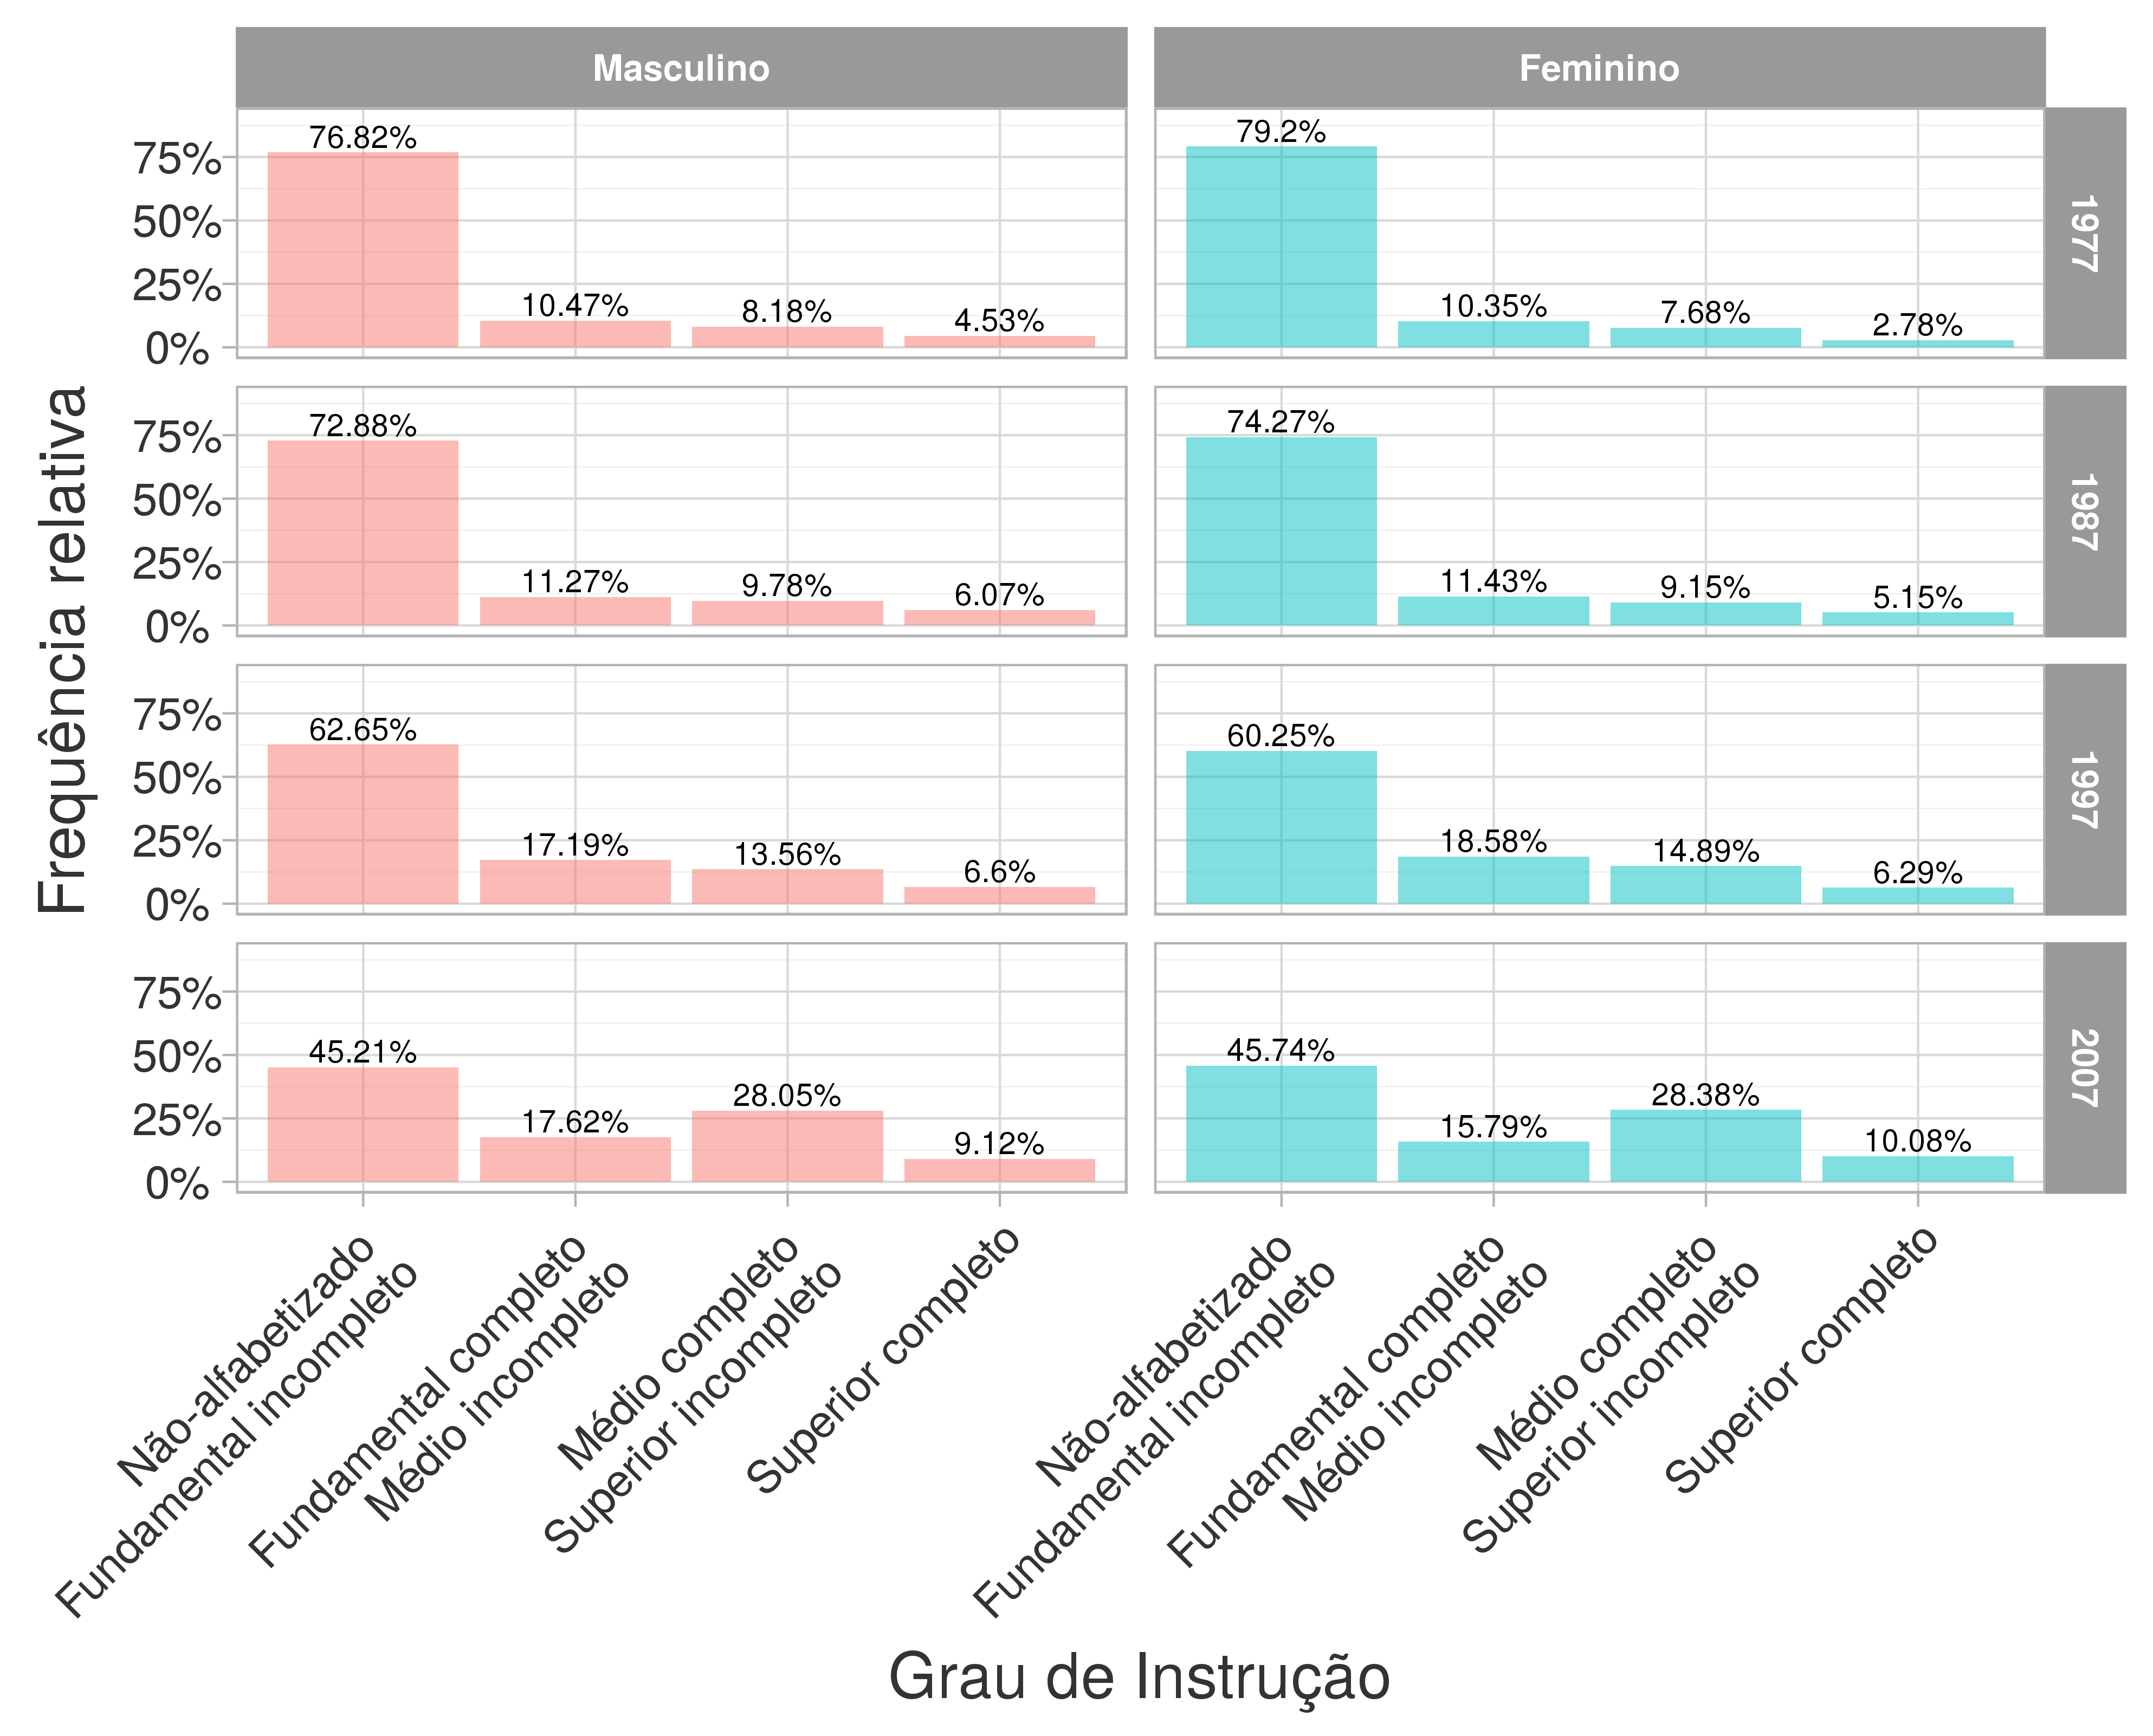
\includegraphics[width=1\textwidth]{./imagens/grau-instr.png}%
    \end{center}%
%    \fonte{Compilação própria}
\end{grafico}%

A elevação do grau de instrução entre 1977 e 2007 influencia não apenas as viagens motivo trabalho (por eventual aumento da empregabilidade) mas também as viagens motivo escola, realizadas por um contingente de pessoas cada vez maior, mais diverso e contendo mais faixas etárias.
A maior participação feminina no mercado de trabalho além de impactar as rendas (individual e familiar) deve influenciar bastante as viagens motivo trabalho. 

A renda individual (variável \textbf{REN_IND}) tem seu comportamento de médias e medianas análogo ao da renda familiar. Explora-se aqui, então, as rendas individuais de quem tem 10 anos ou mais
\footnote{Foi adotada essa idade como limite de corte porque o IBGE produz estatísticas de ``valor do rendimento nominal médio mensal e mediano mensal para pessoas de 10 anos ou mais de idade, total e com rendimento''. Fonte: \url{http://www.sidra.ibge.gov.br/bda/tabela/listabl.asp?c=1381&z=cd&o=7} Acesso em 15 de janeiro de 2016}, 
segmentando por sexo e e por duas situações familiares: pessoa responsável e cônjuge/companheiro(a).
Em todos anos, a renda individual média masculina é superior à feminina para a mesma situação familiar, conforme Tabela \ref{tab:estat-ren-ind}. 
Em 1977, quando pessoa responsável pela família, o homem ganhava 2,5 vezes mais que a mulher em mesma condição. Essa marca vem caindo (cada vez mais devagar) até que, em 2007, eles ganham 1,5 vezes mais do que elas.
Para a situação de cônjuges, a relação entre as rendas médias masculina e feminina giram em média em torno de dois, oscilando para 1,8 em 1987 e 2,4 em 1997. Ou seja, homens cônjuges em geral ganham cerco do dobro das mulheres cônjuges e essa situação pouco se alterou com o passar das décadas.

\begin{table}[htb]
\centering
   \IBGEtab{%\renewcommand{\arraystretch}{1.5}%%\ABNTEXfontereduzida%
        \renewcommand{\arraystretch}{1.5}
        \caption{Estatísticas da variável ``REN_IND''}
        \label{tab:estat-ren-ind}
    }{%

    \begin{tabular}{ccccccc}
        \toprule
        \textbf{Homem} & \multicolumn{3}{c}{\textbf{pessoa responsável}} & \multicolumn{3}{c}{\textbf{cônjuge/companheiro}} \\ \hline
        \textbf{ANO}   & \textbf{Média} & \textbf{Desvio Padrão} & \textbf{Mediana} & \textbf{Média} & \textbf{Desvio Padrão} & \textbf{Mediana} \\ \midrule \midrule
        \textbf{1977}  & 2.762,85 & 3.910,71 & 1.478,21 &   703,24 & 1.461,49 &   0,00 \\ \hline
        \textbf{1987}  & 1.610,76 & 2.146,33 &   985,80 &   522,67 &   953,85 &  99,64 \\ \hline
        \textbf{1997}  & 1.769,16 & 3.272,09 &   873,61 & 1.143,30 & 2.115,36 & 485,34 \\ \hline
        \textbf{2007}  & 1.265,37 & 2.330,39 &   600,00 & 1.147,71 & 2.396,79 & 300,00 \\ \hline                
        \textbf{Total} & 1.869,37 & 3.059,03 &   970,68 & 1.098,29 & 2.280,25 & 291,73 \\\bottomrule

        \textbf{Mulher} & \multicolumn{3}{c}{\textbf{pessoa responsável}} & \multicolumn{3}{c}{\textbf{cônjuge/companheira}} \\ \hline
        \textbf{ANO}   & \textbf{Média} & \textbf{Desvio Padrão} & \textbf{Mediana} & \textbf{Média} & \textbf{Desvio Padrão} & \textbf{Mediana} \\ \midrule \midrule
        \textbf{1977}  & 1.098,95 & 2.108,50 & 506,81 & 306,95 & 1.097,29 & 0,00 \\ \hline
        \textbf{1987}  &   807,79 & 1.398,68 & 397,99 & 284,87 &   872,94 & 0,00 \\ \hline
        \textbf{1997}  & 1.034,83 & 1.923,79 & 465,93 & 478,78 & 1.332,07 & 0,00 \\ \hline
        \textbf{2007}  &   866,43 & 1.661,52 & 380,00 & 498,39 & 1.204,76 & 0,00 \\ \hline                
        \textbf{Total} &   926,53 & 1.752,55 & 388,27 & 383,26 & 1.131,58 & 0,00 \\\bottomrule

    \end{tabular}
    
    }

\end{table}
% Estatísticas para registros com F_PESS==1, filtors em IDADE (>9), SEXO e SIT_FAM
% Não expandido com FE_PESS

\begin{grafico}[htb]%
    \caption{\label{graf:clas-econ-ren-ind}Distribuição da variável ``FAIXA_REN_IND'', por ano}%
        \begin{center}%
        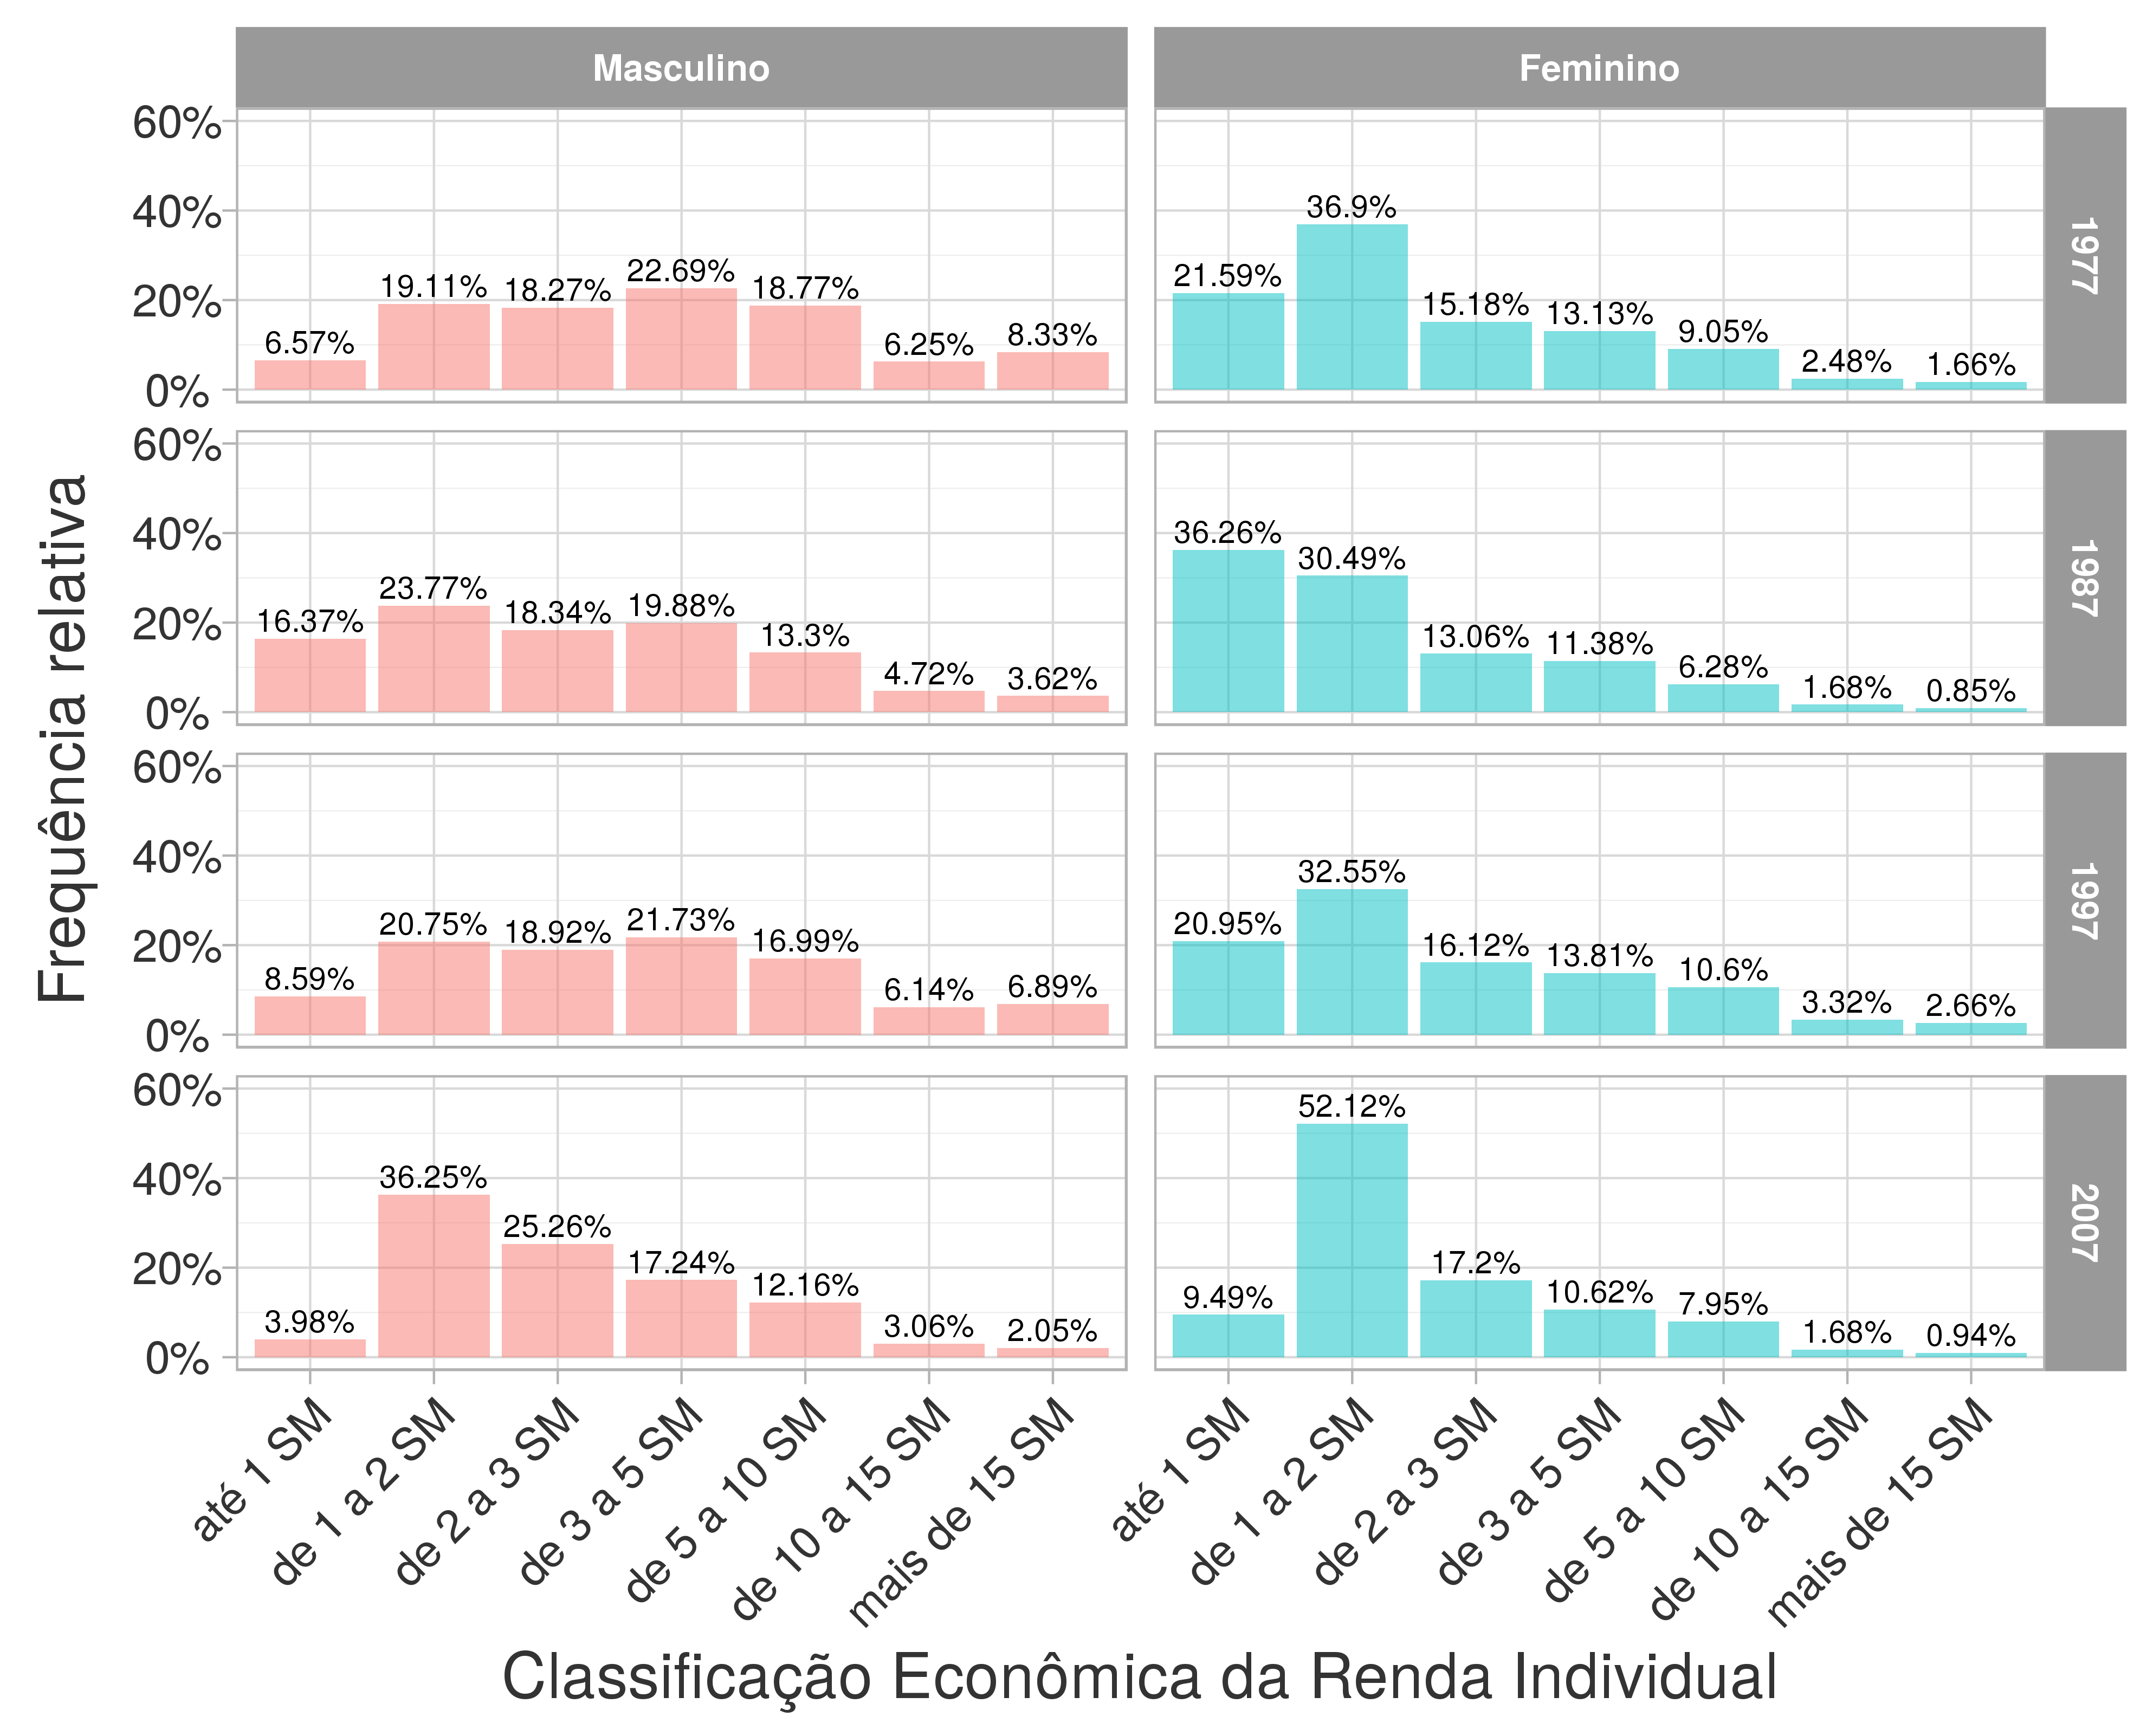
\includegraphics[width=1\textwidth]{./imagens/clas-econ-ren-ind.png}%
    \end{center}%
    %\fonte{Compilação própria}
\end{grafico}%

Pelo Gráfico \ref{graf:clas-econ-ren-ind} percebe-se que houve um aumento de quem ganhava até 1 salário mínimo entre 1977 e 1987. De 1987 para 2007 a proporção de pessoas que têm rendimentos nessa faixa salarial vem decrescendo. De 1977 a 1997 a faixa de rendimento de 1 a 2 salários mínimos ficou próxima dos 25\% e, em 2007, cresceu aproximadamente 10\%. A faixa de rendimento de 2 a 3 salários mínimos subiu cerca de 3\% entre 1977 e 2007, o mesmo que a faixa de rendimentos de 3 a 5 salários mínimos diminuiu no período.


\clearpage

\section{Análises Preliminares}\label{sec:analises-preliminares}

O grupo de análises que se segue busca compreender como é o comportamento das pessoas e das famílias em termo de viagens realizadas, em cada ano e diferencialmente entre os anos, olhando para tanto variáveis como:
\begin{compactitem}
\item número de viagens;
\item modos de viagem;
\item motivos de viagens;
\item duração das viagens;
\item distâncias das viagens.
\end{compactitem}

A variável \textbf{TOT_VIAG} representa o número total de viagens realizadas pela pessoa. Não existem \textit{missing values} neste campo, os valores mínimos para todos anos e ambos sexo são 0, bem como também são 0 os valores do primeiro quartil (25\%). Os valores das demais estatísticas (considerando os fatores de expansão para a população) estão apresentados na Tabela \ref{tab:estat-tot-viag}. Conforme já era de se esperar, para quem faz viagem no dia da pesquisa (número de viagem é não nulo) existe a predominância do valor 2, ou seja, são pessoas que saem de suas residências com um propósito único (trabalhar, estudar, fazer compras) e depois retornam à residência após a atividade.
Percebe-se que, independente do sexo, o número médio de viagens por pessoa em relação a 1977 caiu um pouco em 1987 e 1997 (de 1,67 para 1,64) e subiu novamente em 2007 (para 1,70). Os desvios padrão caíram ao longo do tempo, indicando tendência de menor dispersão dos dados. Os valores de assimetria são positivos, indicando maior concentração à esquerda e cauda longa à direita da distribuição. Os valores de curtose evidenciam não tratar-se de distribuição normal.

Analisando esses dados segmentados por sexo, vê-se que as medianas são iguais. O número médio e máximo de viagens para mulheres é sempre inferior ao dos homens, para o mesmo ano. Os valores de assimetria para o sexo feminino e o masculino são positivos e convergem para o valor geral com o passar das décadas. 
A diferença entre o número médio de viagens de mulheres e homens vem diminuindo.

\begin{table}[htb]
\centering
   \IBGEtab{%\renewcommand{\arraystretch}{1.5}%%\ABNTEXfontereduzida%
        \renewcommand{\arraystretch}{1.5}
        \caption{Estatísticas da variável ``TOT_VIAG'', por ano e por sexo}
        \label{tab:estat-tot-viag}
    }{%

    \begin{tabular}{ccccccc}
        \toprule
        \textbf{Geral} & \multicolumn{3}{c}{\textbf{}} & \multicolumn{3}{c}{\textbf{}} \\ \hline
        \textbf{ANO}   & \textbf{Média} & \textbf{Desvio Padrão} & \textbf{Mediana} & \textbf{Máximo} & \textbf{Assimetria} & \textbf{Curtose} \\ \midrule \midrule
        \textbf{1977}  & 1,67 & 1,75 & 2,00 & 24 & 1,48 & 4,71 \\ \hline
        \textbf{1987}  & 1,64 & 1,61 & 2,00 & 24 & 1,37 & 4,80 \\ \hline
        \textbf{1997}  & 1,64 & 1,60 & 2,00 & 21 & 1,36 & 4,38 \\ \hline
        \textbf{2007}  & 1,70 & 1,48 & 2,00 & 18 & 1,09 & 3,53 \\\bottomrule          

        \textbf{Sexo Feminino} & \multicolumn{3}{c}{\textbf{}} & \multicolumn{3}{c}{\textbf{}} \\ \hline
        \textbf{ANO}   & \textbf{Média} & \textbf{Desvio Padrão} & \textbf{Mediana} & \textbf{Máximo} & \textbf{Assimetria} & \textbf{Curtose} \\ \midrule \midrule
        \textbf{1977}  & 1,35 & 1,58 & 2,00 & 16 & 1,35 & 3,16 \\ \hline
        \textbf{1987}  & 1,42 & 1,58 & 2,00 & 19 & 1,40 & 4,14 \\ \hline
        \textbf{1997}  & 1,52 & 1,62 & 2,00 & 18 & 1,48 & 5,00 \\ \hline
        \textbf{2007}  & 1,61 & 1,51 & 2,00 & 17 & 1,10 & 2,88 \\\bottomrule
        
        \textbf{Sexo Masculino} & \multicolumn{3}{c}{\textbf{}} & \multicolumn{3}{c}{\textbf{}} \\ \hline
        \textbf{ANO}   & \textbf{Média} & \textbf{Desvio Padrão} & \textbf{Mediana} & \textbf{Máximo} & \textbf{Assimetria} & \textbf{Curtose} \\ \midrule \midrule
        \textbf{1977}  & 2,01 & 1,85 & 2,00 & 24 & 1,52 & 5,31 \\ \hline
        \textbf{1987}  & 1,88 & 1,61 & 2,00 & 24 & 1,41 & 5,83 \\ \hline
        \textbf{1997}  & 1,78 & 1,58 & 2,00 & 21 & 1,26 & 3,87 \\ \hline
        \textbf{2007}  & 1,81 & 1,44 & 2,00 & 18 & 1,12 & 4,48 \\\bottomrule             
       
    \end{tabular}
    }{%
%		\fonte{Elaboração própria}
	}
\end{table}
% Estatísticas para registros com F_PESS==1, filtro por SEXO
% Expandido com FE_PESS

Ao considerar apenas quem faz viagens, os valores mínimos para todos anos e ambos sexo passam para 1, bem como também são 1 os valores do primeiro quartil (25\%). Os valores das demais estatísticas (considerando os fatores de expansão para a população) estão apresentados na Tabela \ref{tab:estat-tot-viag-nao-nula}.
Para todos anos e para ambos sexos, as médias passaram para valores superiores a 2 e há uma tendência de diminuição do número de viagens por pessoa com o passar do tempo.
Os desvios padrão caíram ao longo do tempo para as mulheres e para o conjunto de homens e mulheres, indicando menor dispersão dos dados. Os valores de assimetria aumentaram e continuaram positivos, indicando maior concentração à esquerda e cauda longa à direita da distribuição. Os valores de curtose também aumentaram e a distribuição continua não sendo aderente à normalidade.
Na segmentação por sexo, as medianas e a quantidade máxima de viagens permanecem iguais.
Entretanto, o número médio de viagens para mulheres era superior ao dos homens em 1977 e 1987. Já em 1997 e em 2007, a média delas passa a ser inferior à deles.

\begin{table}[htb]
\centering
   \IBGEtab{%\renewcommand{\arraystretch}{1.5}%%\ABNTEXfontereduzida%
        \renewcommand{\arraystretch}{1.5}
        \caption{Estatísticas da variável ``TOT_VIAG'', por ano e por sexo, considerando apenas quem fez viagem}
        \label{tab:estat-tot-viag-nao-nula}
    }{%

    \begin{tabular}{ccccccc}
        \toprule
        \textbf{Geral} & \multicolumn{3}{c}{\textbf{}} & \multicolumn{3}{c}{\textbf{}} \\ \hline
        \textbf{ANO}   & \textbf{Média} & \textbf{Desvio Padrão} & \textbf{Mediana} & \textbf{Máximo} & \textbf{Assimetria} & \textbf{Curtose} \\ \midrule \midrule
        \textbf{1977}  & 2,75 & 1,44 & 2,00 & 24 & 2,70 & 11,75 \\ \hline
        \textbf{1987}  & 2,61 & 1,27 & 2,00 & 24 & 3,01 & 14,66 \\ \hline
        \textbf{1997}  & 2,58 & 1,27 & 2,00 & 21 & 2,89 & 12,59 \\ \hline
        \textbf{2007}  & 2,49 & 1,11 & 2,00 & 18 & 2,94 & 12,77 \\\bottomrule          

        \textbf{Sexo Feminino} & \multicolumn{3}{c}{\textbf{}} & \multicolumn{3}{c}{\textbf{}} \\ \hline
        \textbf{ANO}   & \textbf{Média} & \textbf{Desvio Padrão} & \textbf{Mediana} & \textbf{Máximo} & \textbf{Assimetria} & \textbf{Curtose} \\ \midrule \midrule
        \textbf{1977}  & 2,85 & 1,57 & 2,00 & 16 & 2,65 & 11,19 \\ \hline
        \textbf{1987}  & 2,61 & 1,29 & 2,00 & 19 & 3,08 & 15,47 \\ \hline
        \textbf{1997}  & 2,56 & 1,26 & 2,00 & 18 & 2,73 & 10,55 \\ \hline
        \textbf{2007}  & 2,47 & 1,09 & 2,00 & 17 & 3,10 & 15,08 \\\bottomrule
        
        \textbf{Sexo Masculino} & \multicolumn{3}{c}{\textbf{}} & \multicolumn{3}{c}{\textbf{}} \\ \hline
        \textbf{ANO}   & \textbf{Média} & \textbf{Desvio Padrão} & \textbf{Mediana} & \textbf{Máximo} & \textbf{Assimetria} & \textbf{Curtose} \\ \midrule \midrule
        \textbf{1977}  & 2,62 & 1,23 & 2,00 & 24 & 2,55 &  9,84 \\ \hline
        \textbf{1987}  & 2,60 & 1,24 & 2,00 & 24 & 2,90 & 13,40 \\ \hline
        \textbf{1997}  & 2,59 & 1,29 & 2,00 & 21 & 3,06 & 14,56 \\ \hline
        \textbf{2007}  & 2,52 & 1,13 & 2,00 & 18 & 2,79 & 10,71 \\\bottomrule             
       
    \end{tabular}
    }{%
%		\fonte{Elaboração própria}
	}
\end{table}
% Estatísticas para registros com F_PESS==1, filtro por SEXO
% Expandido com FE_PESS

Foram feitos testes t para avaliar se as médias de mulheres e de homens eram estatisticamente diferentes, em cada ano, tanto considerando quem não fez viagem (TOT_VIAG=0), com desconsiderando esse caso. Os p-valores resultantes foram todos inferiores a 0,05, logo, rejeitou-se a hipótese nula de que as médias seriam iguais (nível de confiança de 95\%).
Foram feitos testes t para avaliar se as médias entre os anos eram diferentes, para o grupo de mulheres, , tanto considerando quem não fez viagem (TOT_VIAG=0), com desconsiderando esse caso. Também aqui os p-valores resultantes foram todos inferiores a 0,05, logo, rejeitou-se a hipótese nula de que as médias seriam iguais (nível de confiança de 95\%). 
Portanto, ao considerar o efeito de quem não sai de casa, o número médio de viagens das mulheres sempre é menor que o dos homens, para um dado ano, e realmente houve aumento no número médio de viagens das mulheres, da ordem de 0,1 viagem/ano.
Ao desconsiderar o efeito de quem não sai de casa, o número médio de viagens das mulheres tornou-se menor que o dos homens em 1997 e o número médio de viagens de homens e mulheres cai com o tempo.

O Gráfico \ref{graf:distr-num-viag} apresenta a distribuição de viagens (considerando os fatores de expansão para a população) até o limite de 6 viagens, corte feito apenas para melhorar a visualização do gráfico, já que a cauda é bastante longa. 
Deste gráfico, vale destacar a relação entre as viagens nulas (quem não sai de casa) e as viagens de ida e volta (valores iguais a 2). Para homens, o número de viagens nulo é menos frequente que o número de viagens de valor 2 para todos anos de análise. Já para as mulheres, em 1977 as viagens nulas eram a maioria, indicando certa fixitude delas na residência. Essa porcentagem vai diminuindo e a porcentagem no número de viagens igual a 2 vai crescendo, ficam próximas em 1997 e, em 2007, inverte-se a situação observada em 1977.
Provavelmente devido à maior participação no mercado de trabalho, as mulheres ganharam mobilidade, restringindo-se menos ao espaço doméstico.

\begin{grafico}[htb]%
    \caption{\label{graf:distr-num-viag}Distribuição da variável ``TOT_VIAG'' por ano e por sexo}%
    \begin{center}%
        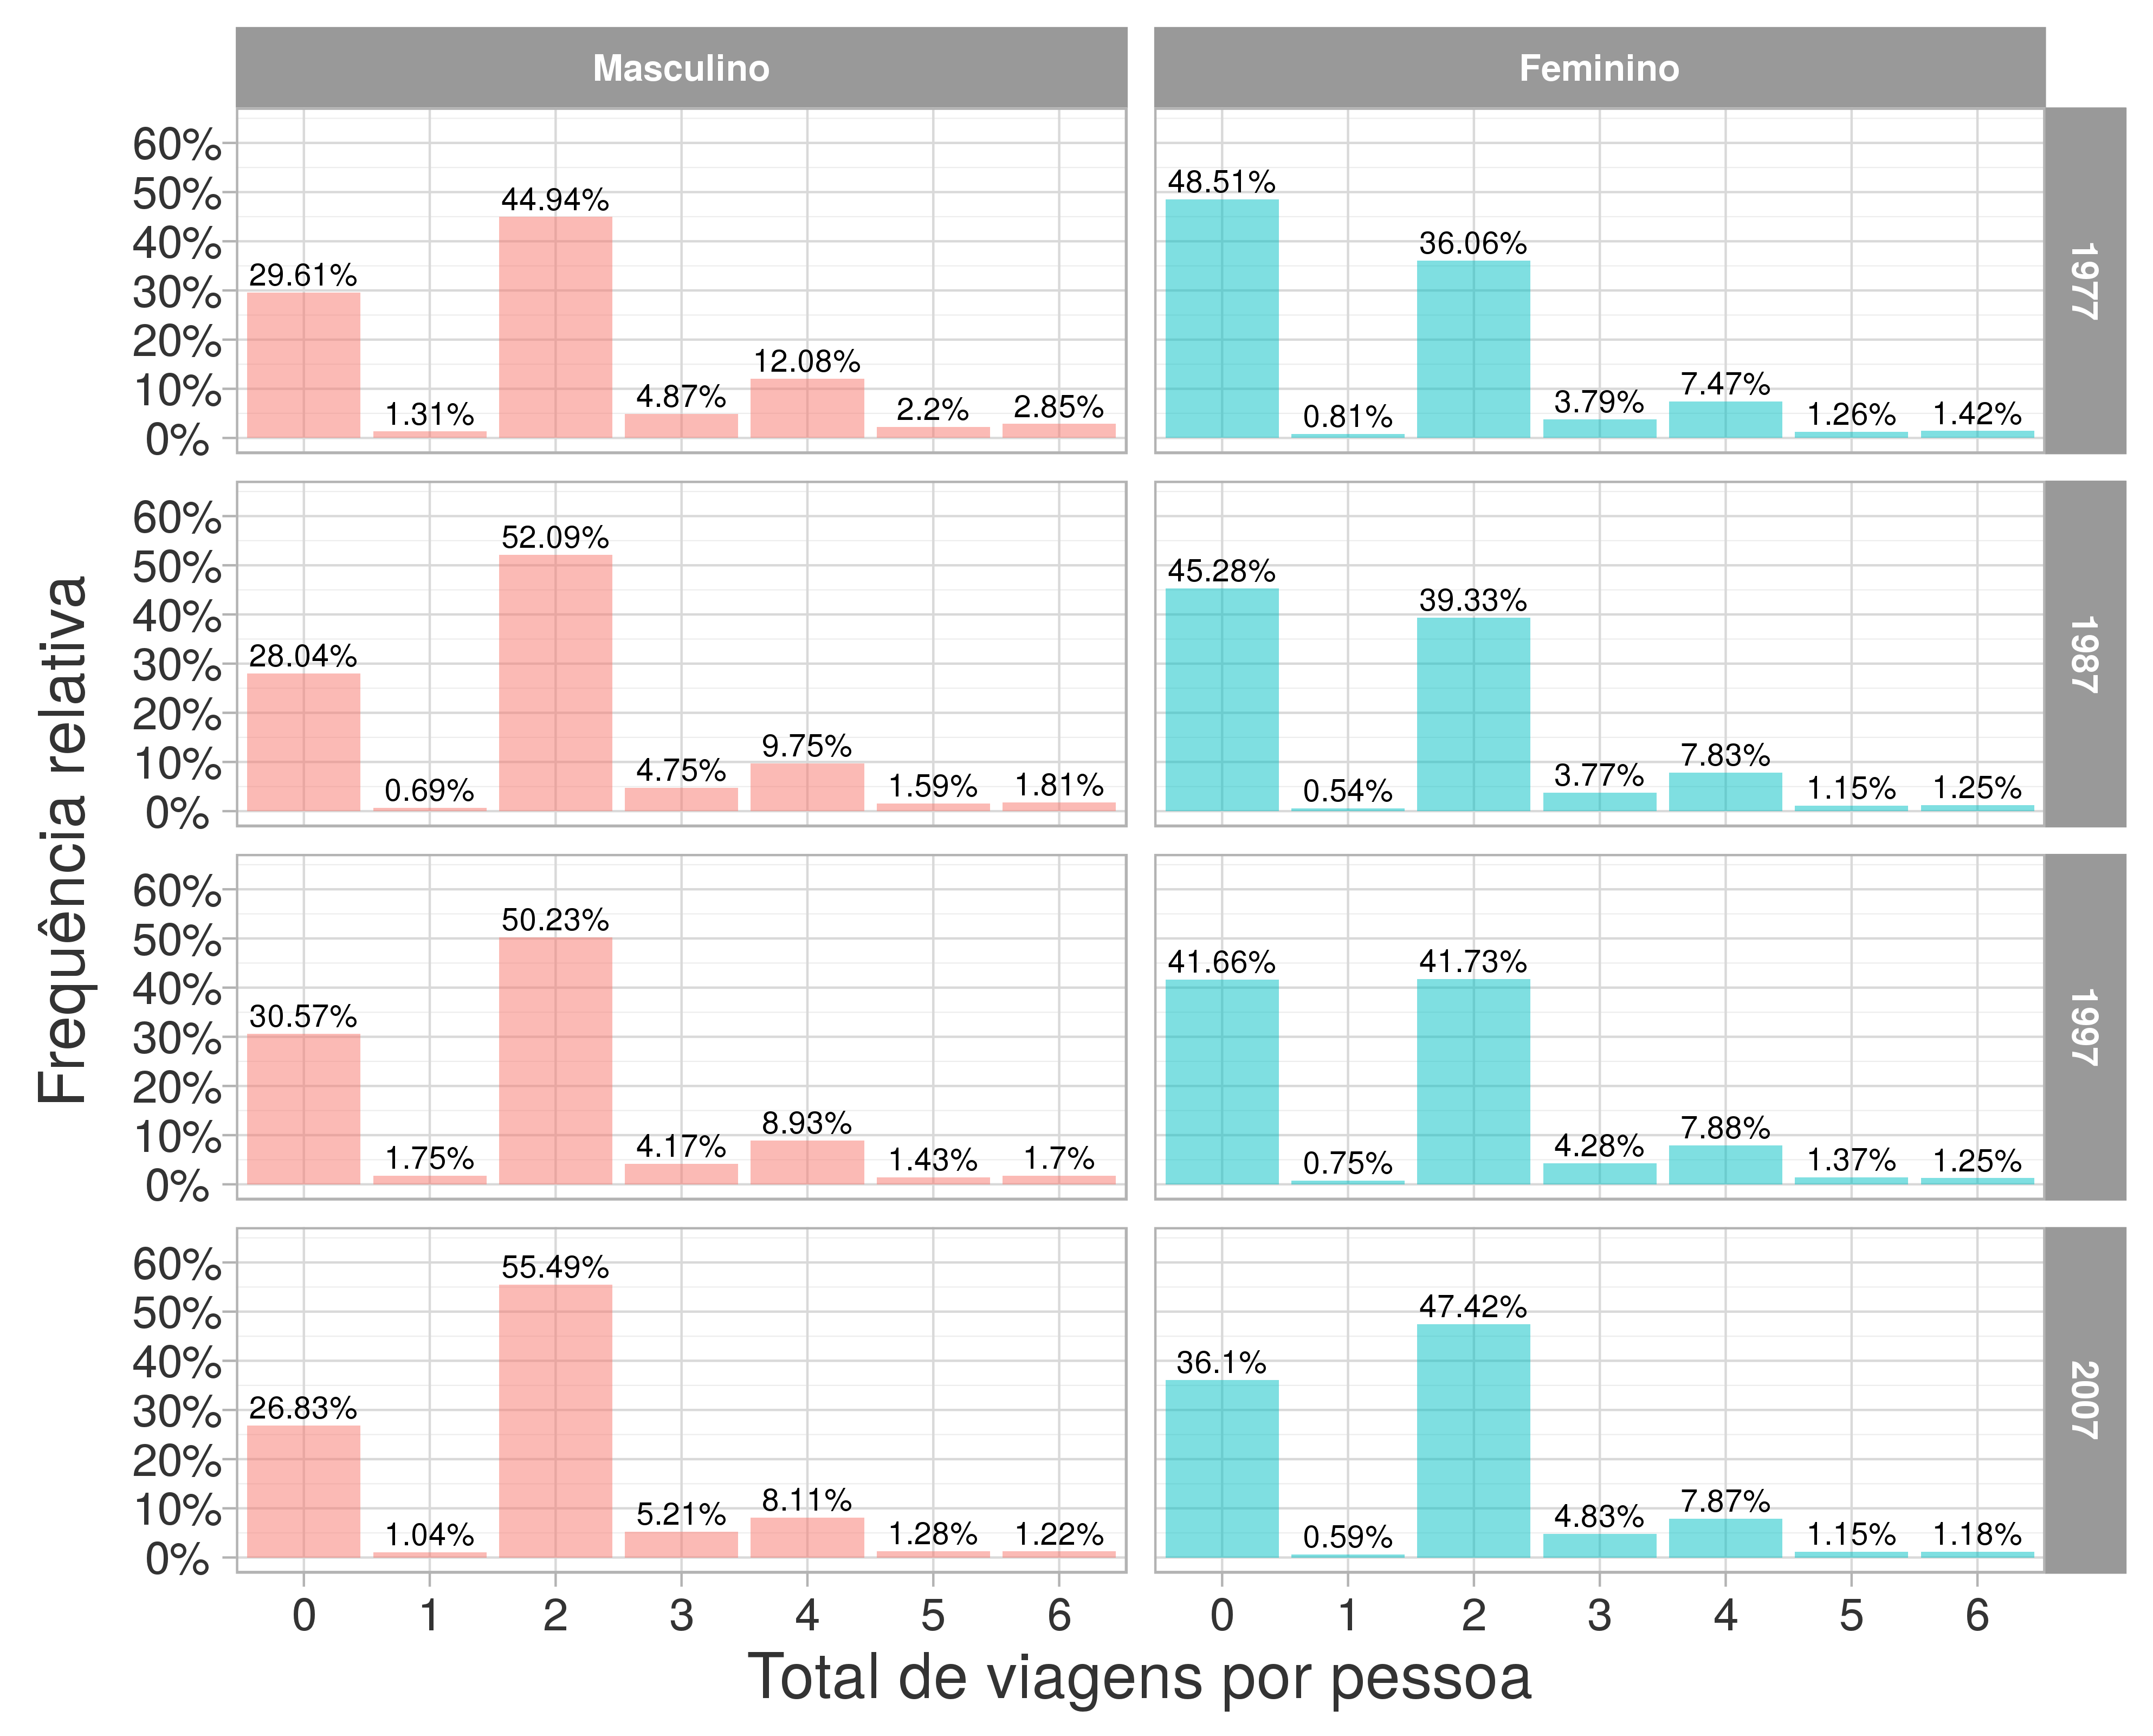
\includegraphics[width=1\textwidth]{./imagens/tot-viag-pess.png}%
    \end{center}%
%    \fonte{Compilação própria}
\end{grafico}%
% Estatísticas para registros com F_PESS==1 e SEXO
% Expandido com FE_PESS

\newpage
Ao focar no agregado da família, os valores das principais estatísticas (considerando os fatores de expansão para a população) da variável \textbf{FAM_VIAG_TOT} estão apresentados na Tabela \ref{tab:estat-fam-viag-tot}.
O número médio de viagens da família com ao longo do tempo, comportamento consistente tanto com a queda do número médio de viagens por pessoa (Tabelas \ref{tab:estat-tot-viag} e \ref{tab:estat-tot-viag-nao-nula}) quanto com a diminuição do tamanho da família (Tabela \ref{tab:estat-tot-pess}).
Aqui também os desvios padrão caem ao longo do tempo (tendência de menor dispersão de dados) e os valores de assimetria são positivos (maior concentração à esquerda e cauda longa à direita da distribuição). Os valores de curtose indicam que a distribuição não é normal.
Ao retirar aquelas famílias com total de viagens nulo (ninguém fez viagem), não se observam diferenças nas tendências das estatísticas, à exceção da mediana que em 1997 era 7 em 1997 e passa para 6 ao inserir famílias cujo total de viagens é zero.

\begin{table}[htb]
\centering
   \IBGEtab{%\renewcommand{\arraystretch}{1.5}%%\ABNTEXfontereduzida%
        \renewcommand{\arraystretch}{1.5}
        \caption{Estatísticas da variável ``FAM_VIAG_TOT'', por ano}
        \label{tab:estat-fam-viag-tot}
    }{%

    \begin{tabular}{ccccccc}
        \toprule
        \textbf{} & \multicolumn{5}{c}{\textbf{Considerando famílias em que há pela menos viagem}} & \multicolumn{1}{c}{\textbf{}} \\ \hline
        \textbf{ANO}   & \textbf{Média} & \textbf{Desvio Padrão} & \textbf{Mediana} & \textbf{Máximo} & \textbf{Assimetria} & \textbf{Curtose} \\ \midrule \midrule
        \textbf{1977}  & 8,97 & 6,00 & 8,00 & 59 & 1,36 & 2,90 \\ \hline
        \textbf{1987}  & 8,04 & 5,14 & 7,00 & 50 & 1,39 & 3,43 \\ \hline
        \textbf{1997}  & 7,68 & 4,80 & 7,00 & 45 & 1,29 & 2,85 \\ \hline
        \textbf{2007}  & 7,11 & 4,31 & 6,00 & 68 & 1,52 & 6,84 \\\bottomrule          

        \textbf{} & \multicolumn{5}{c}{\textbf{Considerando inclusive família em que ninguém fez viagem}} & \multicolumn{1}{c}{\textbf{}} \\ \hline
        \textbf{ANO}   & \textbf{Média} & \textbf{Desvio Padrão} & \textbf{Mediana} & \textbf{Máximo} & \textbf{Assimetria} & \textbf{Curtose} \\ \midrule \midrule
        \textbf{1977}  & 8,58 & 6,14 & 8,00 & 59 & 1,27 & 2,62 \\ \hline
        \textbf{1987}  & 7,71 & 5,28 & 7,00 & 50 & 1,27 & 3,05 \\ \hline
        \textbf{1997}  & 7,22 & 5,00 & 6,00 & 45 & 1,14 & 2,39 \\ \hline
        \textbf{2007}  & 6,62 & 4,53 & 6,00 & 68 & 1,28 & 5,38 \\\bottomrule

    \end{tabular}
    }{%
%		\fonte{Elaboração própria}
	}
\end{table}
% Estatísticas para registros com F_FAM==1, filtro por ANO
% Expandido com FE_FAM

\newpage
Nos campos MODO1, MODO2, MODO3 e MODO4 a categoria ``ônibus de linha'' inclui as categorias originais ``ônibus trólebus'', ``trólebus'', ``ônibus diesel'', ``ônibus'', ``ônibus município de São Paulo'', ``ônibus outros municípios'' e ``ônibus metropolitano''. A categoria ``ônibus escolar/empresa'' inclui também as categorias originais ``ônibus fretado'', ``escolar'', ``transporte escolar``. A categoria ``lotação/van'' inclui as categorias originais ``lotação/perua'', ``microônibus/van município de São Paulo'', ``microônibus/van outros municípios'' e ``microônibus/van metropolitano''. Vale destacar que para os anos de 1977 e 1987 foram levantados no máximo três modos, e para os anos 1997 e 2007, no máximo quatro modos para cada viagem.

Na Tabela \ref{tab:estat-modos} foram agrupados em ``alta capacidade'' os modos metroferroviários (metrô e trem), em ``ônibus'' todos os tipos de ônibus (de linha, escolar, de empresas, lotações e vans), em ``passageiro de automóvel'' os passageiros de automóvel particular e também de táxis, em ``Outros'' as viagens realizadas por motocicletas e bicicletas pois estas foram diagnosticadas apenas para 2007. Nesta tabela estão apresentadas as frequências relativas destes agrupamentos para o \textbf{MODO1} (primeiro modo utilizado na viagem) e também para o \textbf{MODO2} (segundo modo utilizado), buscando avaliar a divisão modal por ano, para quem realizou viagem. Assim, para o primeiro modo o total soma 100\% em todos anos, mas o total por ano do segundo modo em diante não necessariamente, porque nem todas viagens utilizaram mais de um modo.


\begin{table}[htb]
\centering
   \IBGEtab{%\renewcommand{\arraystretch}{1.5}%%\ABNTEXfontereduzida%
        \renewcommand{\arraystretch}{1.5}
        \caption{Frequência relativa das variáveis ``MODO1'' e ``MODO2'', por ano}
        \label{tab:estat-modos}
    }{%

    \begin{tabular}{cccccccc}
        \toprule
        \textbf{MODO 1} & \textbf{Alta}       & \textbf{}       & \textbf{Dirigindo} &  \textbf{Passageiro}  & \textbf{}     & \textbf{}  & \textbf{} \\
        \textbf{ANO}    & \textbf{Capacidade} & \textbf{Ônibus} & \textbf{Automóvel} & \textbf{de Automóvel} & \textbf{A pé} & \textbf{Outros} & \textbf{Total} \\ \midrule \midrule
        \textbf{1977}  & 3,0\% & 41,7\% & 15,4\% & 11,3\% & 28,0\% & 0,8\% & 100\% \\ \hline
        \textbf{1987}  & 4,7\% & 30,5\% & 17,2\% &  9,7\% & 36,2\% & 1,7\% & 100\% \\ \hline
        \textbf{1997}  & 6,4\% & 28,9\% & 20,5\% & 10,8\% & 34,4\% & 1,3\% & 100\% \\ \hline
        \textbf{2007}  & 7,0\% & 31,8\% & 19,2\% &  8,6\% & 33,1\% & 2,9\% & 100\% \\\bottomrule          

        \textbf{MODO 2}      & \textbf{Alta}       & \textbf{}       & \textbf{Dirigindo} &  \textbf{Passageiro}  & \textbf{}     & \textbf{}  & \textbf{} \\
        \textbf{ANO}   & \textbf{Capacidade} & \textbf{Ônibus} & \textbf{Automóvel} & \textbf{de Automóvel} & \textbf{A pé} & \textbf{Outros} & \textbf{Total} \\ \midrule \midrule
        \textbf{1977}  & 2,0\% & 7,0\% & 0,1\% & 0,2\% & - & 0,0\% &  9,2\% \\ \hline
        \textbf{1987}  & 3,6\% & 6,5\% & 0,1\% & 0,1\% & - & 0,0\% & 10,3\% \\ \hline
        \textbf{1997}  & 3,5\% & 5,9\% & 0,0\% & 0,1\% & - & 0,0\% &  9,5\% \\ \hline
        \textbf{2007}  & 4,2\% & 8,2\% & 0,1\% & 0,1\% & - & 0,0\% & 12,5\% \\\bottomrule    
      
    \end{tabular}
    }{%
%		\fonte{Elaboração própria}
	}
\end{table}
% Estatísticas para registros com F_VIAG==1
% Expandido com FE_VIAG

Em relação à utilização do automóvel, sua proporção sobe cerca de 5\% de 1977 até 1997 e cai pouco mais de 1\% em 2007, talvez por conta dos congestionamentos cada vez mais frequentes e da evolução do sistema de transporte coletivo público da RMSP. Quando utilizado, o carro é quase sempre o único modo da viagem.
Os ônibus têm uma queda de $\sim$ 13\% pontos percentuais entre 1977 e 1997, com recuperação de $\sim$ 3\% em 2007. Quem deixou de utilizar o ônibus nas primeiras 3 décadas passou a utilizar a caminhada como método de deslocamento ($\sim$ 6\%), ou o carro ($\sim$ 5\%) o ainda o transporte coletivo de alta capacidade ($\sim$ 3\%).
Os modos metrô e trem vêm recebendo um incremento de viagens década a década, saindo de 3\% em 1977 para 7\% em 2077. A contribuição baixa deste modo, apesar de sua alta capacidade, deve-se provavelmente à cobertura insuficiente de pouca capilaridade no tecido urbano.
Vale ressaltar que ``alta capacidade'' é o único modo que tem sua utilização ainda muito presente como segundo modo (relação MODO1/MODO2 $\sim$ 1,5) - as viagens de ônibus são reduzidas pelo menos da ordem de um quarto, as de carro e outros caem a quase 0\% no segundo modo.
Isto significa que as viagens com metrô e trem são mais frequentemente precedidas de viagens com outro modo (principalmente ônibus), funcionando como tronco numa lógica de sistema tronco-alimentador.
As viagens a pé aumentaram percentualmente entre 1977 e 1997 e caíram em 2007, talvez pelas distâncias necessárias de viagem dado o crescimento da área metropolitana de São Paulo. Conforme o conceito de viagem a pé anteriormente exposto, não haverá modo a pé nos modos 2, 3 ou 4.
As tabelas de contingência dos modos 3 e 4 não serão apresentadas por serem pouco significativos no contexto geral: o modo 3 varia de 0,9\% (em 1977) a 2,8\% (2007) do total de viagens, sendo predominante o modo ônibus; o modo 4, só existente em 1997 e 2007, corresponde ao total de 0,4\% das viagens realizadas.

Os Gráficos \ref{graf:freq-modo1} e \ref{graf:freq-modo2} apresentam a segmentação por sexo dos modos 1 e 2 de viagem, respectivamente.
No primeiro modo de viagem, as viagens a pé são o modo mais frequente para as mulheres em 1987, 1997 e 2007, somente em 1977 o ônibus era mais frequentemente utilizado por elas.
Para os homens o modo mais frequente em 1977 e 2007 é o ônibus, e em 1987 e 1997, a pé.
O modo outros é o menos frequente em 1977, 1987 e 1997 para ambos sexos; em 2007, eles superam a alta capacidade, provavelmente porque a expressividade do transporte por motocicleta e bicicleta passou a ser mais expressiva e foi incluída na categoria outros.
Comparando ambos sexos por categoria do primeiro modo:
\begin{compactitem}[]
\item (i) As mulheres sempre fizeram mais viagens a pé que os homens: a diferença de 6,7 pontos percentuais de 1977 aumenta para 11,3 em 1987, cai para 7,9 em 1997 e sobe novamente em 2007 para 8,8\%.
\item (ii) A utilização feminina do ônibus é quase sempre superior á masculina, exceto em 1987, ano em que as proporções praticamente se igualam e desde quando a diferença vem aumentando com o tempo.
\item (iii) É na utilização do automóvel em que residem as diferenças mais gritantes entre os gêneros: homens predominantemente motoristas e mulheres, passageiras. O destaque aqui reside no fato que entre 1997 e 2007, dentro do grupo de mulheres, elas passaram a dirigir mais do que ser passageiras de automóvel.
\item (iv) O transporte de alta capacidade gira em torno de 2,5\% a 5,5\% do \textit{share} modal, com o homem tendo uma utilização um pouco mais frequente dentro do seu grupo do que as mulheres, mais devido ao trem (cujos percentuais dos homens são sempre superiores aos das mulheres) do que ao Metrô (onde os percentuais das mulheres supera o dos homens a partir de 1997).
\end{compactitem}

\begin{grafico}[htb]%
    \caption{\label{graf:freq-modo1}Proporção das viagens do sexo feminino e do sexo masculino, segundo o primeiro modo da viagem, por ano}%
    \begin{center}%
        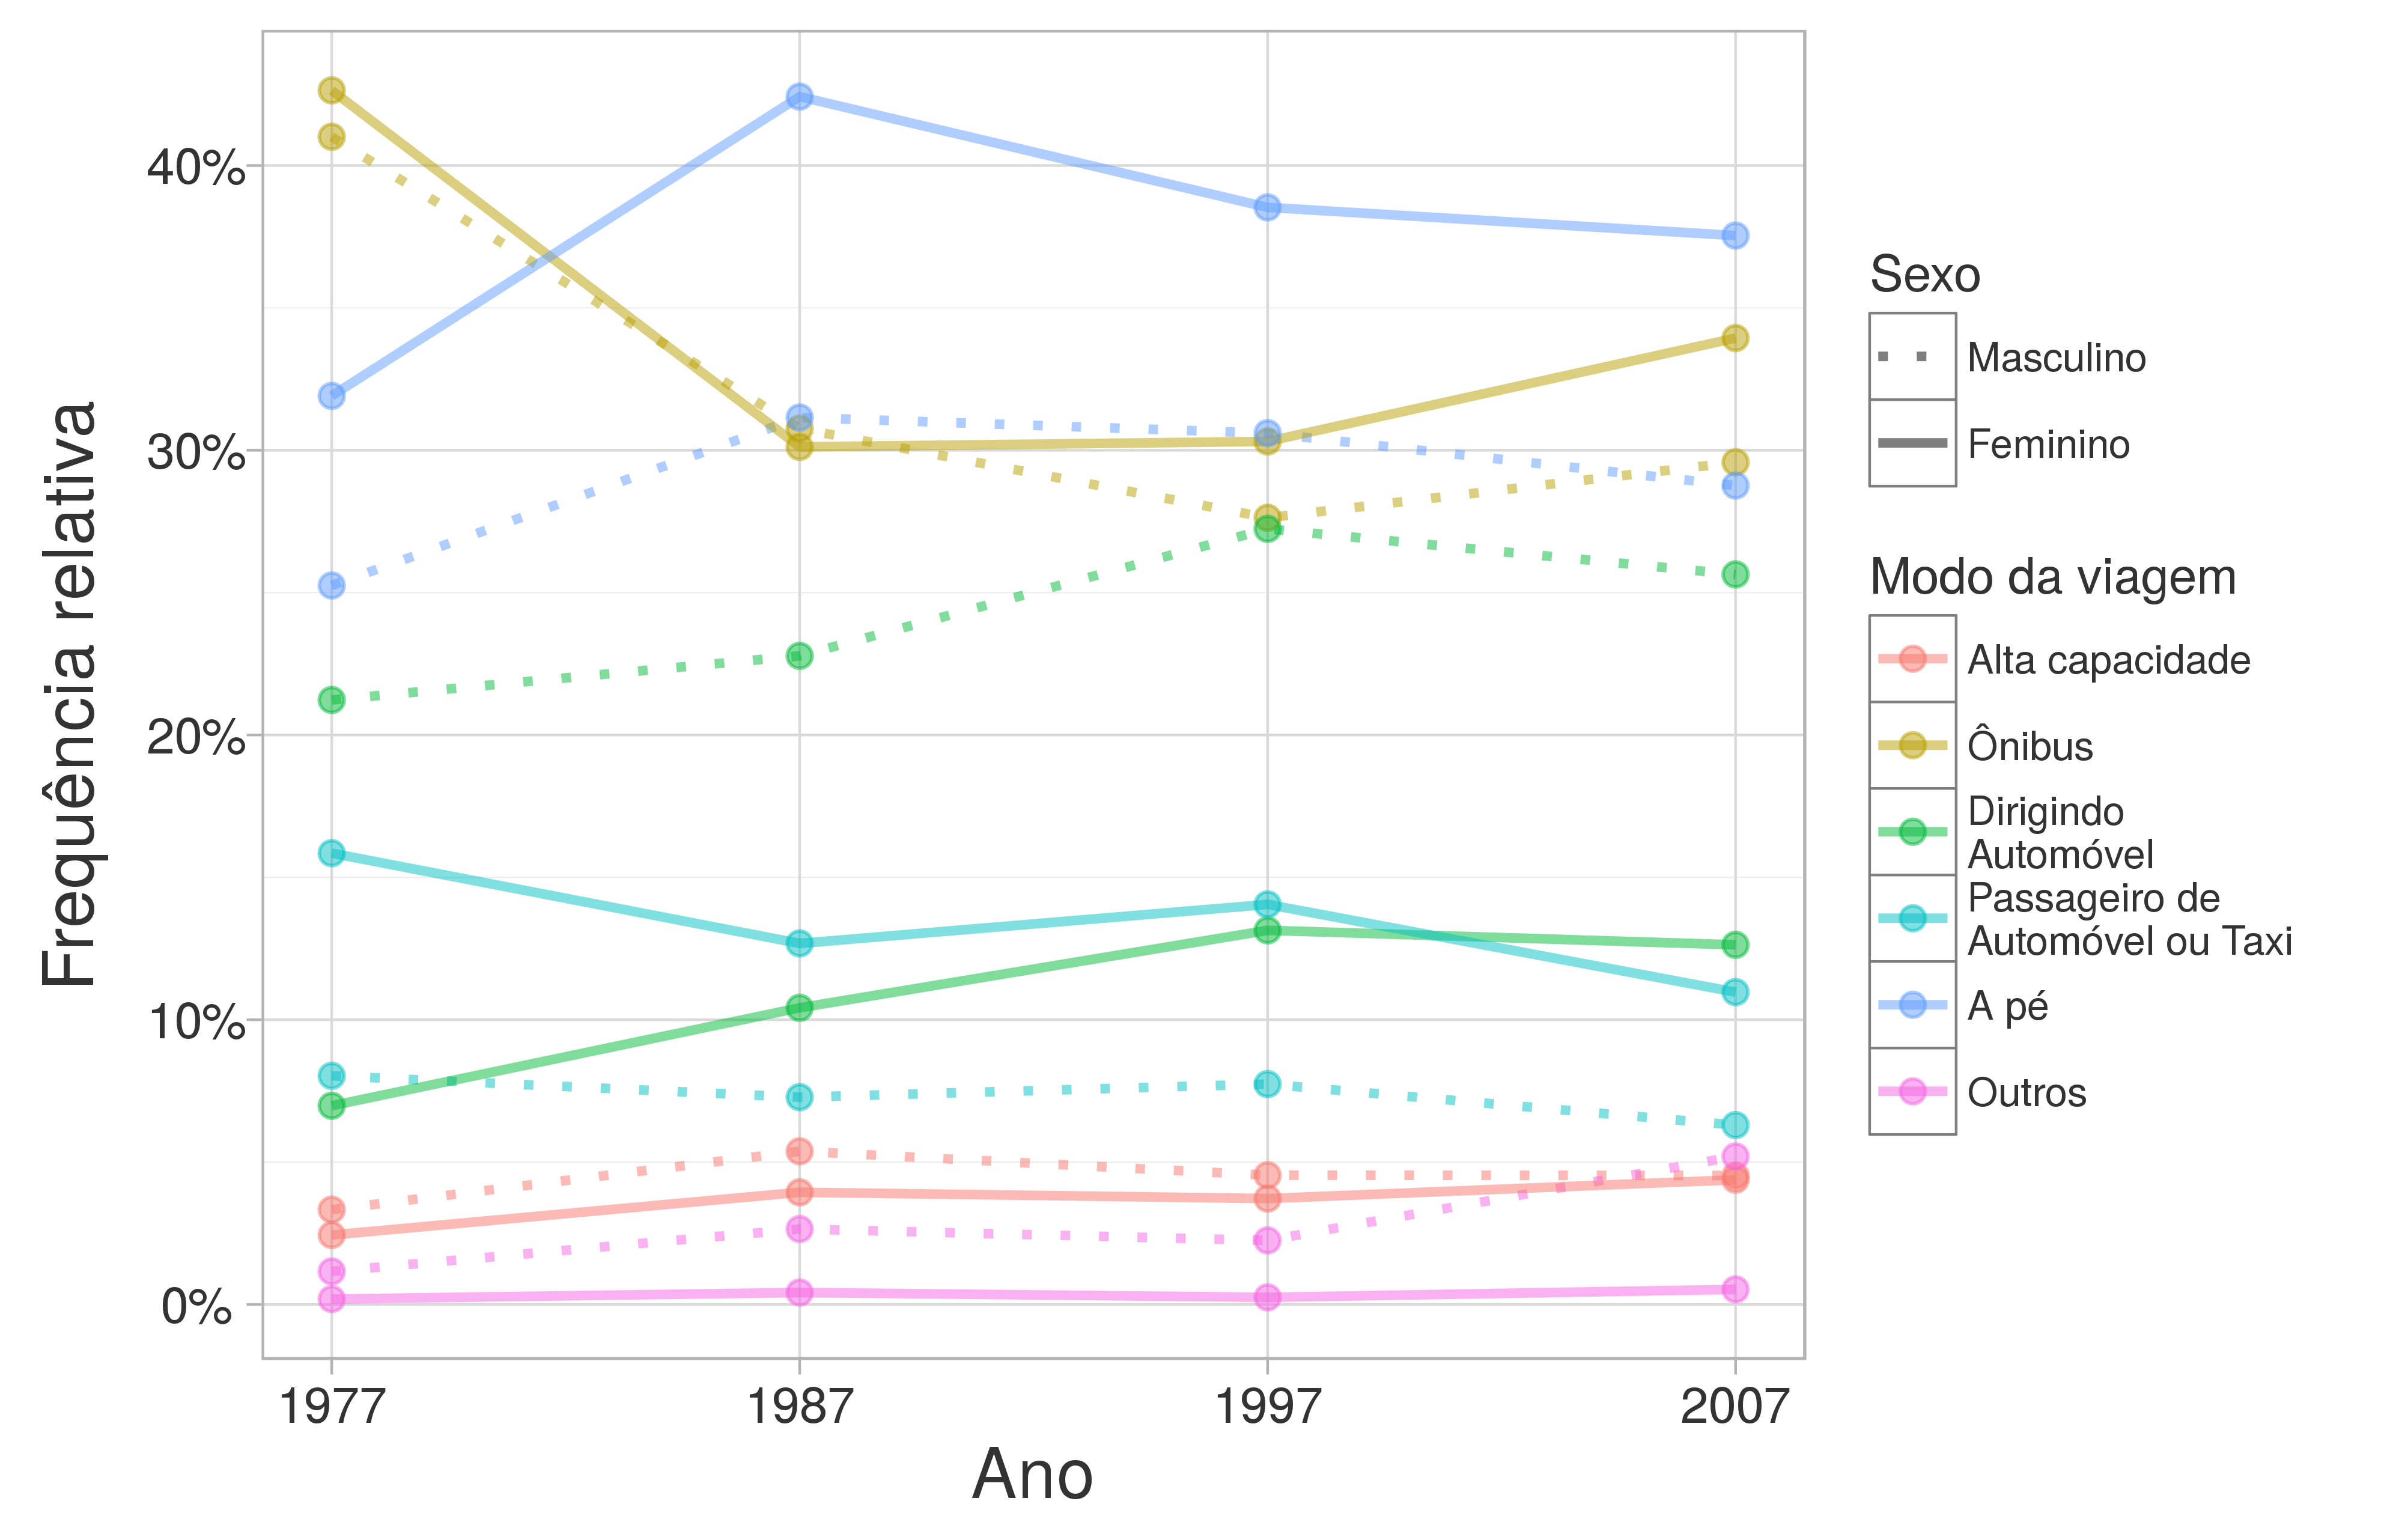
\includegraphics[width=1\textwidth]{./imagens/freq-modo1.png}%
    \end{center}%
%    \fonte{Compilação própria}
\end{grafico}%
% Estatísticas para registros com F_VIAG==1 e SEXO
% Expandido com FE_VIAG

Analisando agora as categorias do segundo modo, por sexo:
\begin{compactitem}[]
\item (i)  As duas categorias que apresentam relevância como segundo modo de transporte equivalem aos modos coletivos ônibus e alta capacidade (metrô e trem), os demais modos ou não foram considerados (por exemplo, a pé) ou não são muito significativos (automóvel e outros).
\item (ii) A utilização feminina do ônibus, como segundo modo da viagem, é inferior à masculina entre 1977 e 1997, ao contrário do que ocorria com o primeiro modo. Em 2007 a situação se altera, quando pessoas do sexo feminino passam a utilizar mais frequentemente o ônibus.
\item (iii) A frequência do uso de alta capacidade é mais expressiva no conjunto do modo 2, embora ainda seja menor que a do ônibus em todos os anos e para ambos sexos.
\item(iv) Para as mulheres, de 1977 para 1987, parece ter havido uma troca modal no segundo modo: houve queda de $\sim$ 1\% no uso do ônibus e aumento também de $\sim$ 1\% no uso de alta capacidade. Foi nesse período em que houve a primeira expansão da rede metroferroviária para a zona leste (trecho Sé-Penha).
\end{compactitem}

\begin{grafico}[htb]%
    \caption{\label{graf:freq-modo2}Proporção das viagens do sexo feminino e do sexo masculino, segundo o segundo modo da viagem, por ano}%
    \begin{center}%
        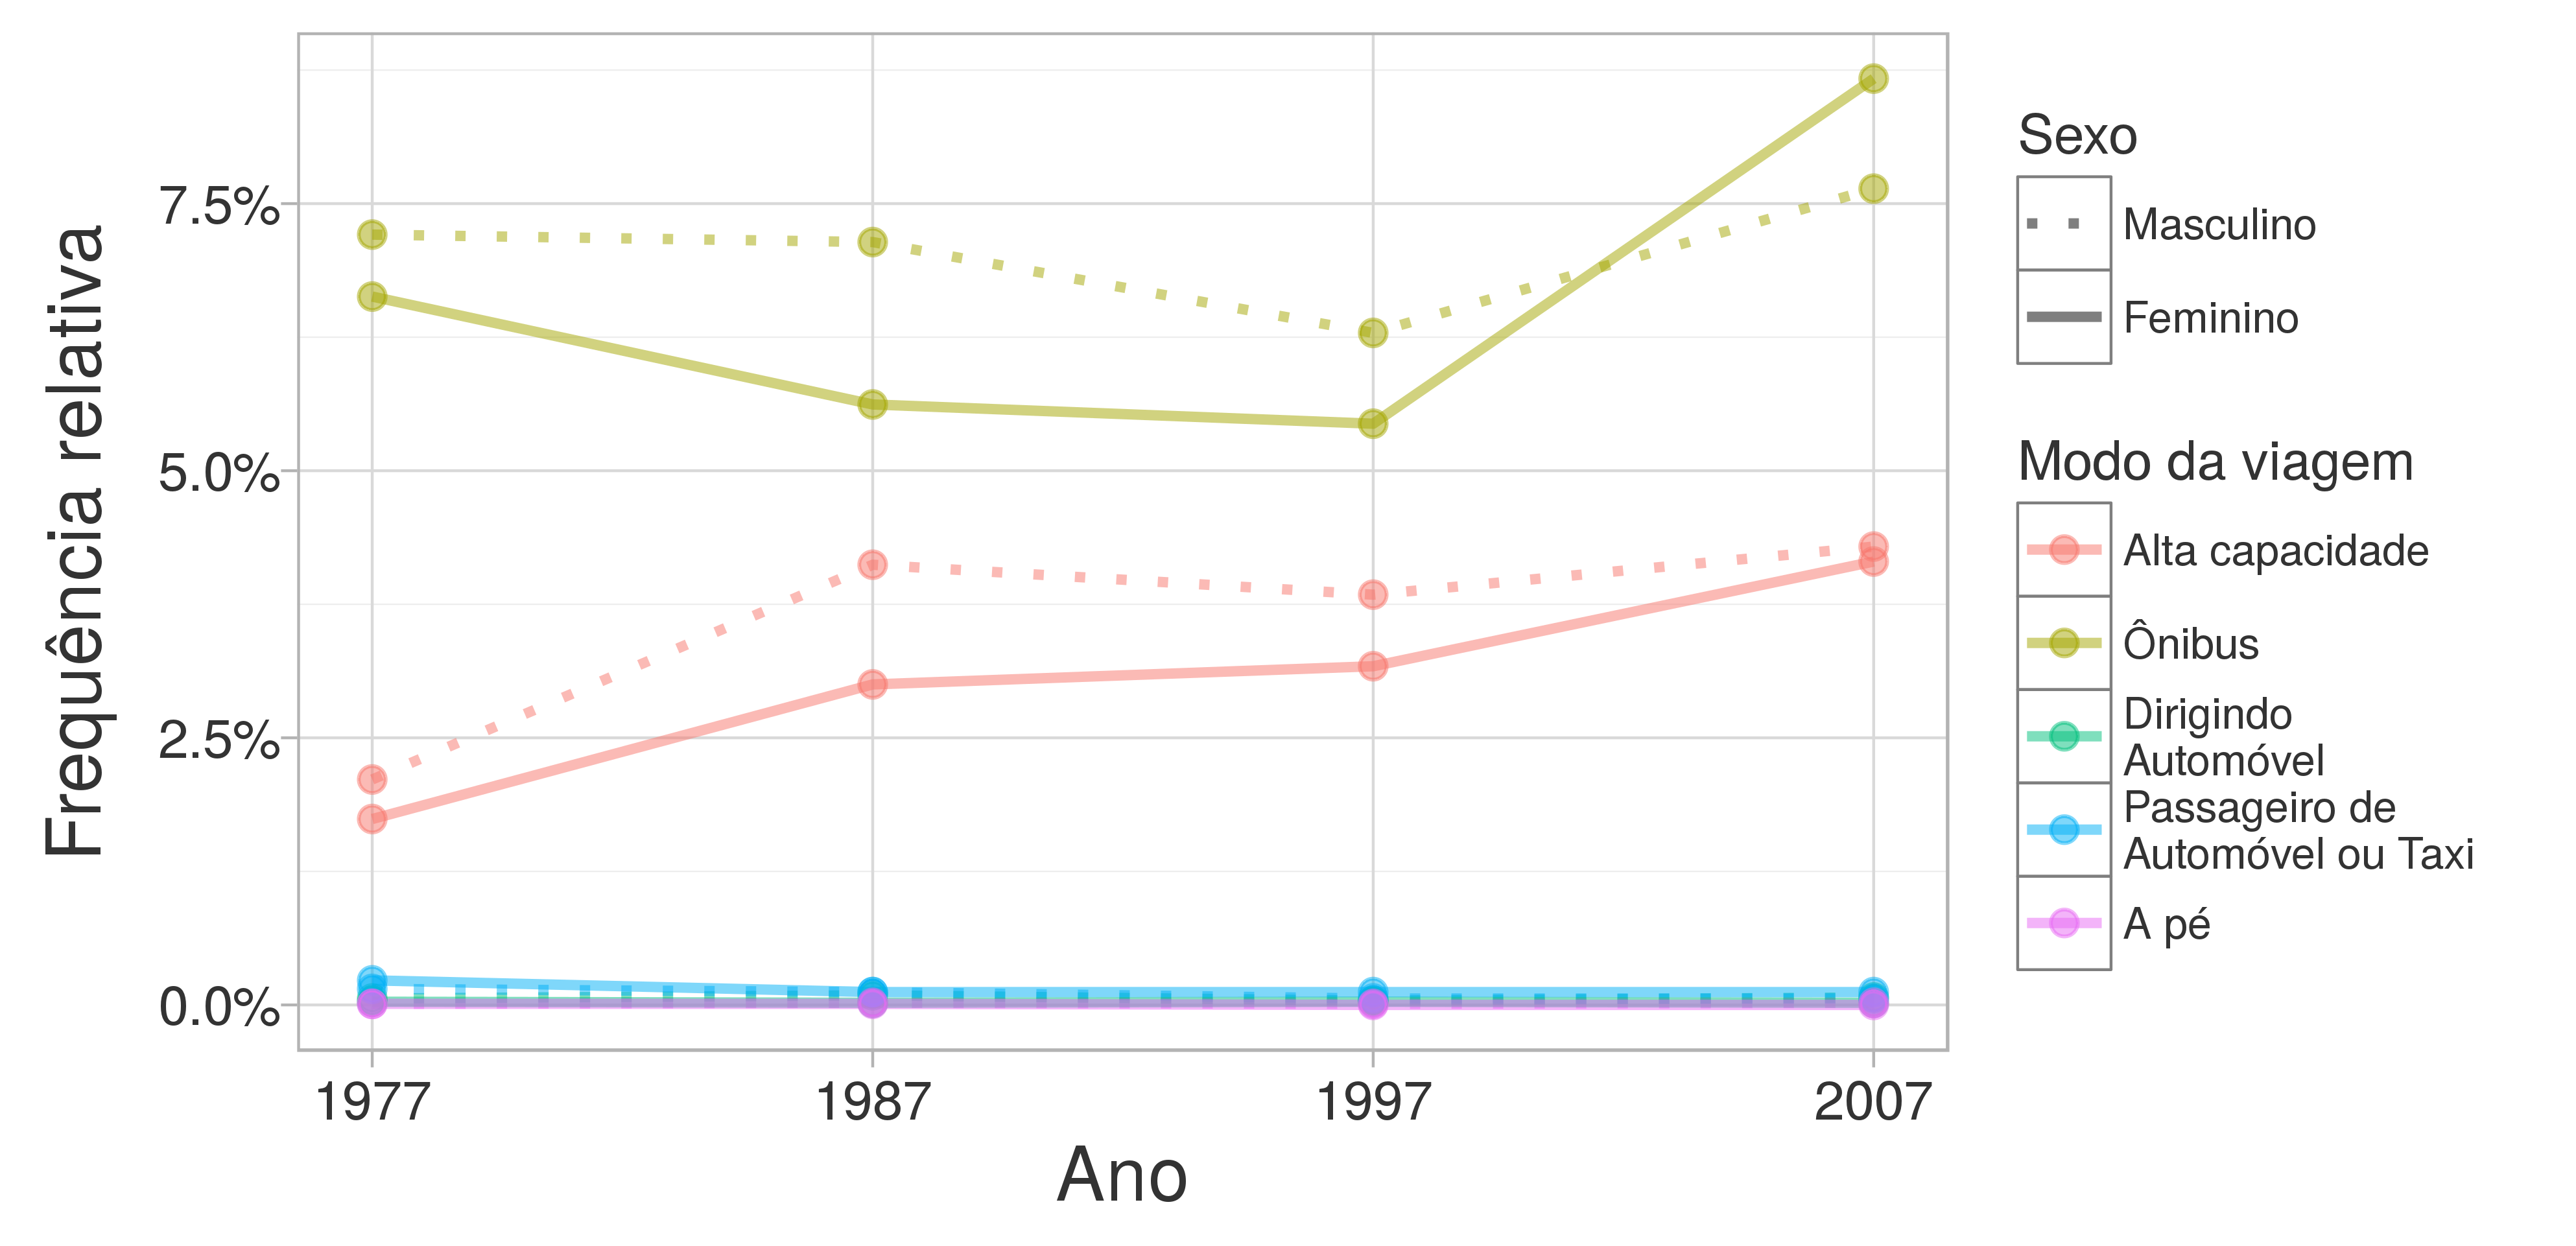
\includegraphics[width=1\textwidth]{./imagens/freq-modo2.png}%
    \end{center}%
%    \fonte{Compilação própria}
\end{grafico}%
% Estatísticas para registros com F_VIAG==1 e SEXO
% Expandido com FE_VIAG

\clearpage

É possível também analisar os modos agregando os modos em ``coletivo'', ``individual'' e ``a pé'', o que já fora feito na variável \textbf{TIPO_VIAG}, cujas frequências relativas são apresentadas na Tabela \ref{tab:estat-tipo-viag}.
O transporte individual cresceu de 1977 a 1997 e recuou um pouco em 2007.
O transporte coletivo decresceu entre 1977 e 1987, mas a uma taxa bem maior que o crescimento do individual, o que significa que essas viagens deixaram de ser feitas de transporte coletivo para, principalmente, serem feitas a pé ou, com menor frequência, de carro.
Entre 1987 a 1997 tanto o transporte coletivo como o modo a pé sofrem ligeiras quedas (em torno de 2 pontos percentuais), período em que o transporte individual aumenta sua taxa de crescimento. Neste ano o cenário da divisão modal fica quase equitativamente dividido com cerca de um terço para cada uma das três categorias.
Em 2007 a forma de deslocamento a pé sofre ligeira queda ($\sim$ 1\%), o transporte individual também cai ($\sim$ 2,5\%) e essas viagens passam a ser feitas pelo transporte coletivo que assume proporção um pouco superior à que tinha em 1987.

\begin{table}[htb]
\centering
   \IBGEtab{%\renewcommand{\arraystretch}{1.5}%%\ABNTEXfontereduzida%
        \renewcommand{\arraystretch}{1.5}
        \caption{Frequência relativa da variável ``TIPO_VIAG'', por ano}
        \label{tab:estat-tipo-viag}
    }{%

    \begin{tabular}{cccc}
        \toprule
        \textbf{ANO}   & \textbf{Coletivo} & \textbf{Individual} & \textbf{A pé} \\ \midrule \midrule
        \textbf{1977}  & 45,0\%            & 27,0\%              & 28,0\%  \\ \hline
        \textbf{1987}  & 35,6\%            & 28,2\%              & 36,2\%  \\ \hline
        \textbf{1997}  & 33,3\%            & 32,3\%              & 34,4\%  \\ \hline
        \textbf{2007}  & 36,5\%            & 29,5\%              & 33,1\%  \\ \bottomrule          
    \end{tabular}
    }{%
%		\fonte{Elaboração própria}
	}
\end{table}
% Estatísticas para registros com F_VIAG==1
% Expandido com FE_VIAG

O Gráfico \ref{graf:freq-tipo-viag} apresentam a segmentação por sexo do modo (agregado) de viagem.
Comparando ambos sexos por categoria do primeiro modo:
\begin{compactitem}[]
\item (i) Em 1977, 45,4\% das mulheres usavam o transporte coletivo, 31,9\% deslocavam-se a pé e 22,7\% usavam transporte individual. Em 1987, para elas, o transporte individual permanece no mesmo patamar ($\sim$ 23,2\%) e ocorre uma migração do coletivo para o a pé com 34,4\% e 42,4\%, respectivamente.
\item (ii) Em 1977, 44,7\% dos homens usavam o transporte coletivo, 30,1\% o individual e 25,3\% deslocavam-se a pé. Em 1987, para eles, o transporte individual cresceu ($\sim$ 32,3\%) e as viagens a pé também ($\sim$ 31,2\%) indicando uma migração do transporte coletivo (36,5\%) para estes modos.
\item (iii) Entre 1987 e 1997, a proporção de mulheres a usar o transporte coletivo permanece inalterada, mas ocorre uma migração do modo a pé para o transporte individual.
\item (iv) Entre 1987 e 1997, a proporção de homens a usar o transporte individual continua aumentando (para 37\%), superando a participação do coletivo (32,4\%), enquanto as viagens a pé permanecem no mesmo patamar.
\item (v) Entre 1997 e 2007, a proporção do uso feminino do transporte coletivo cresce (para 38,7\%) indicando migração para este modo das viagens advindas, especialmente, do transporte individual (que cai para 23,6\%) e, em menor medida, do modo a pé (com 37,5\%). 
\item (vi) Entre 1997 e 2007, a proporção do uso masculino do transporte coletivo também cresce (para 34,4\%) indicando migração para este modo das viagens advindas tanto do transporte individual (que cai para 35,4\%) como do modo a pé (com 28,8\%).
\end{compactitem}
% Em 2007 não fecha 100% porque havia no banco uns casos de TIPO_VIAG=4, cujo significado desconheço pois valor não consta do layout

\begin{grafico}[htb]%
    \caption{\label{graf:freq-tipo-viag}Proporção das viagens do sexo feminino e do sexo masculino, segundo o modo da viagem (agregado), por ano}%
    \begin{center}%
        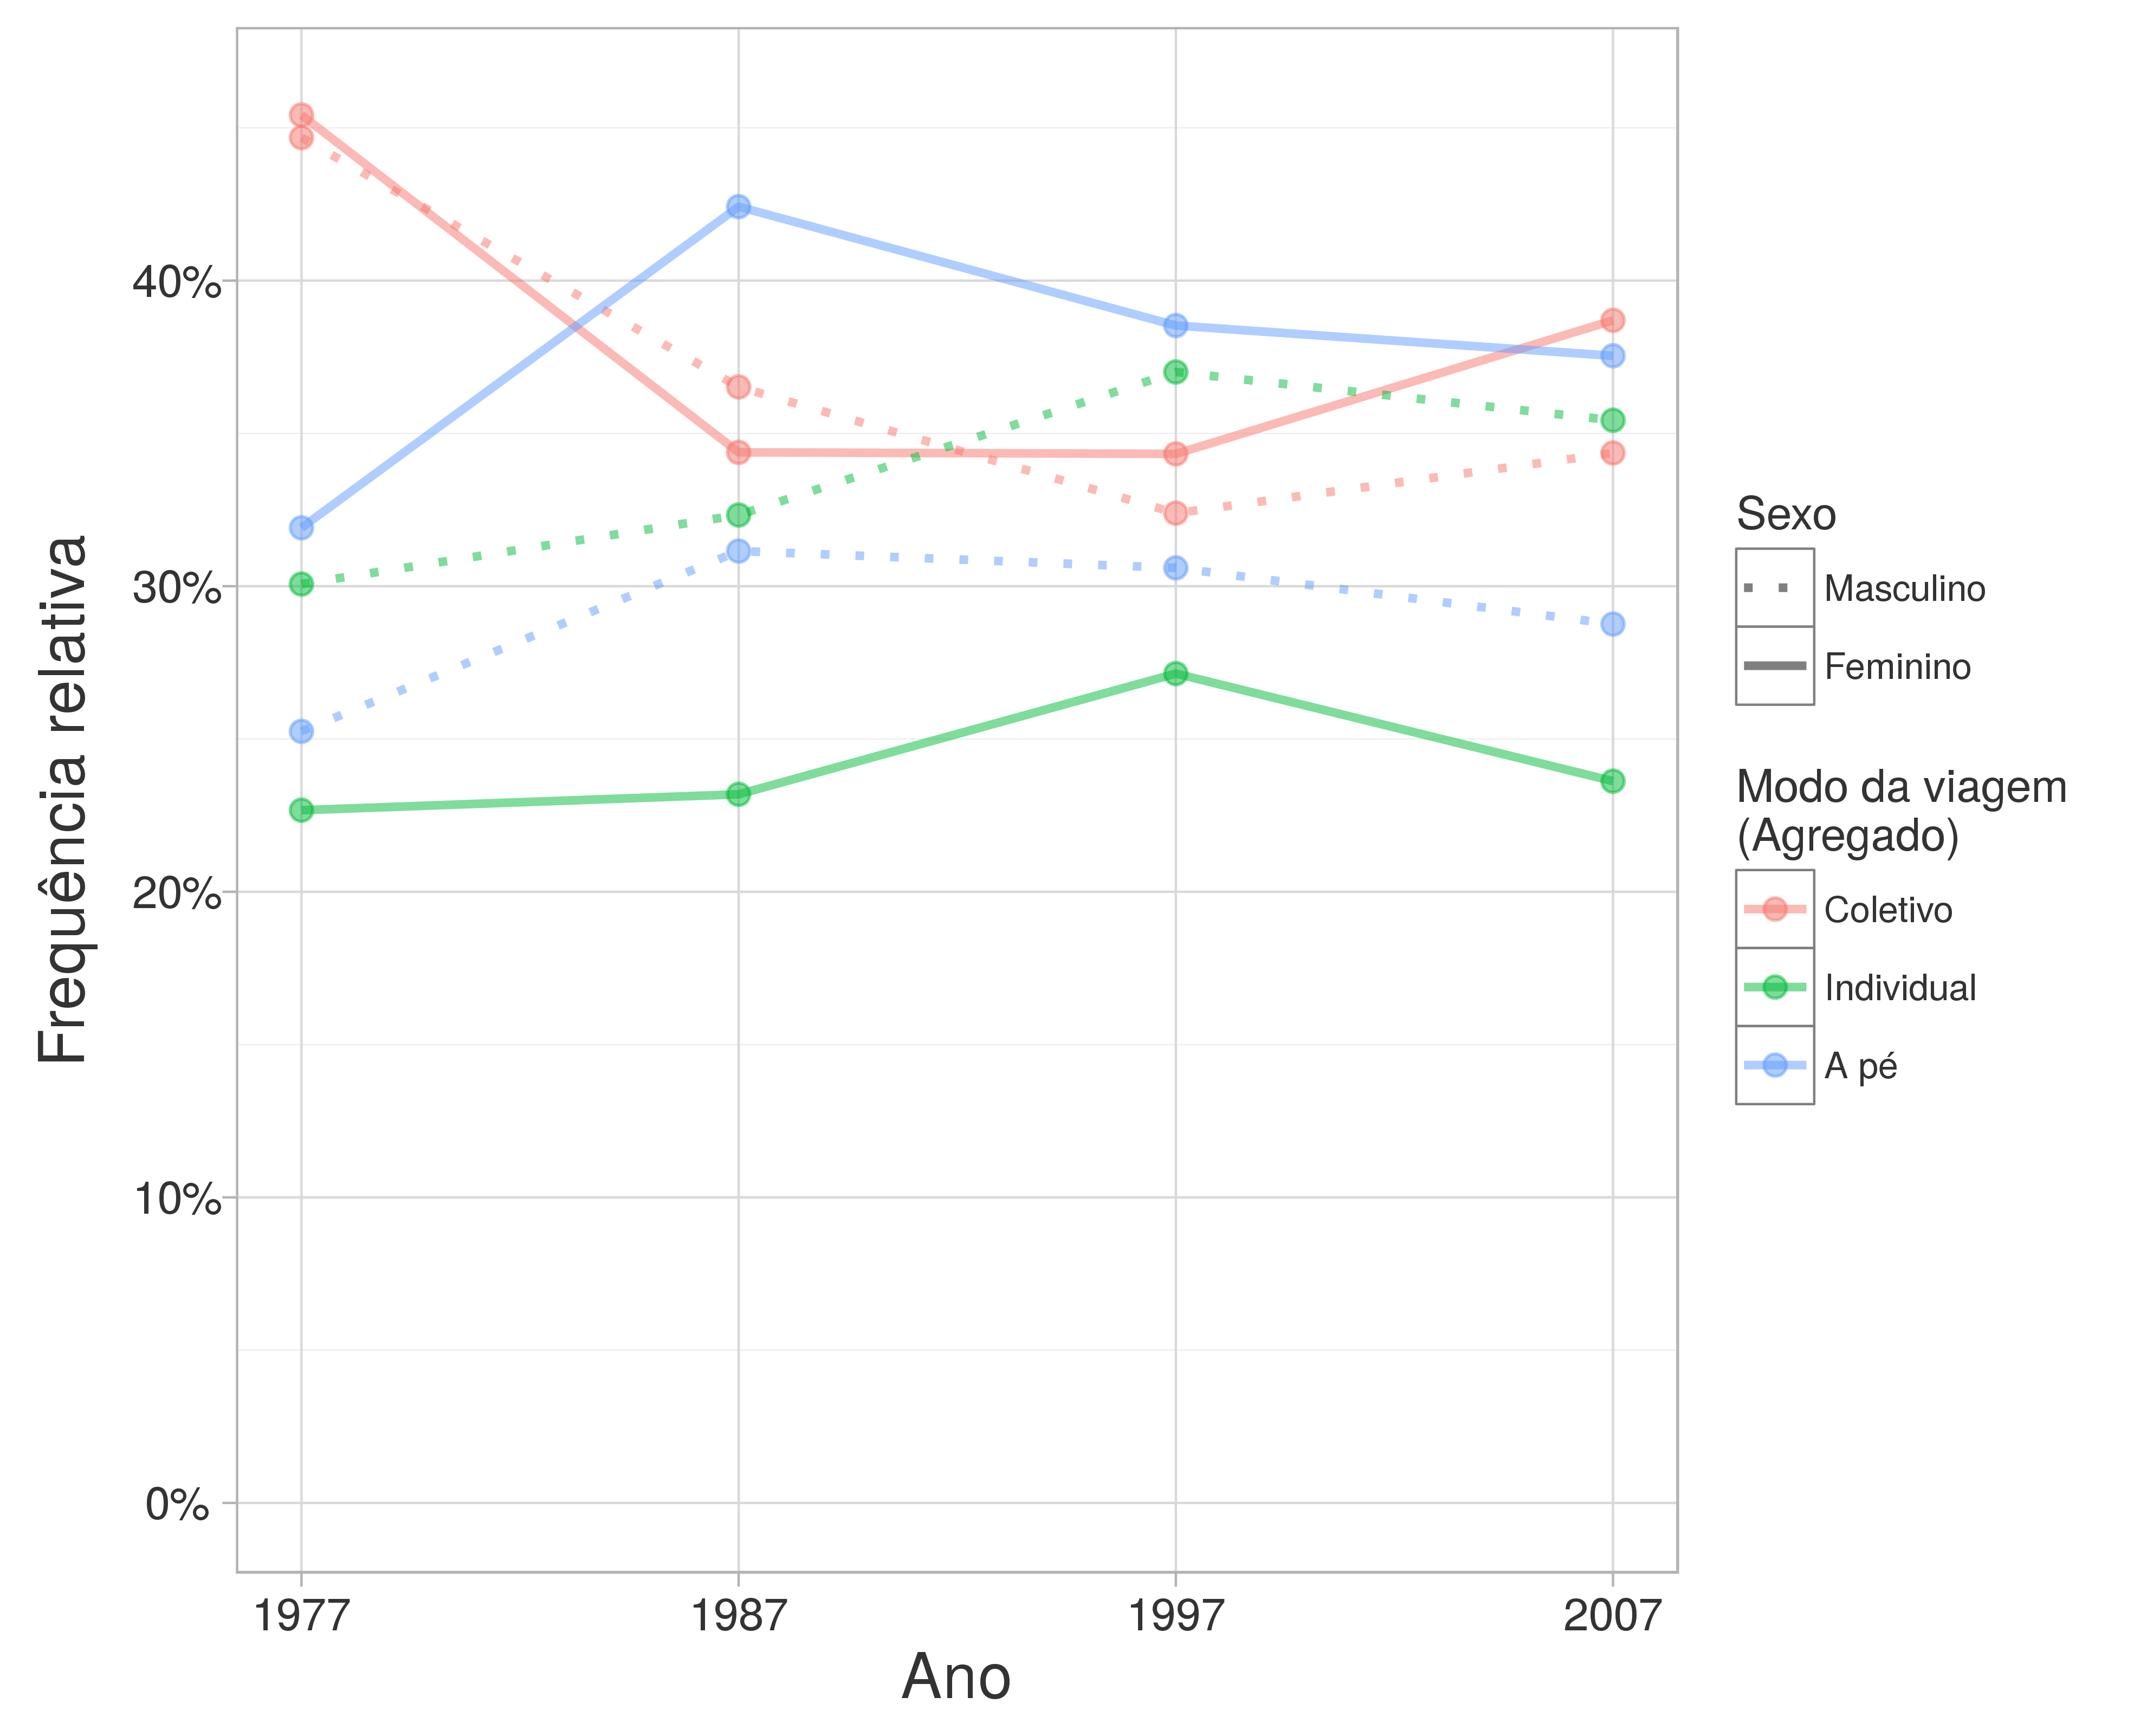
\includegraphics[width=1\textwidth]{./imagens/freq-tipo-viag.png}%
    \end{center}%
%    \fonte{Compilação própria}
\end{grafico}%
% Estatísticas para registros com F_VIAG==1 e SEXO
% Expandido com FE_VIAG

Para as variáveis de motivo (\textbf{MOTIVO_ORIG} e \textbf{MOTIVO_DEST}) foi criada a categoria ``servir passageiro''. Para tanto, olhava-se a variável de cada OD ``servir passageiro na origem''; caso fosse afirmativo (1), a categoria adotada é ``servir passageiro'', porque o que motiva esse deslocamento é o motivo de outrem, não o da pessoa respondente. Caso contrário, adota-se o motivo de origem indicado originalmente na base de dados. Tal procedimento foi realizado com as bases de 1997 e 2007. A base de 1977 já conta com a categoria ``servir passageiro''. A base de 1987 é a única que não possui informações suficientes para identificar esse motivo de viagem.

Será explorada a variável motivo no destino porque essa variável indica a atividade fim que gerou o deslocamento.
A Tabela \ref{tab:estat-motivo-dest} foi feita expandindo as viagens com o FE_VIAG, consequentemente consideradas apenas as viagens realizadas (cujo FE_VIAG não foram iguais a zero).
Observa-se que o motivo ``residência'' corresponde à maior parte das viagens (cerca de 45\%) realizadas, se alterando pouco ao longo dos anos - resultado próximo ao esperado (pouco menos de 50\%) dado que o comportamento de deslocamentos da demanda tem a residência como base, ou seja, é para onde a maior parte das pessoas retornam após executar alguma outra atividade.
O segundo motivo mais frequente é ``trabalho'' girando em torno dos 23,5\% e também oscilando pouco (1\%) ao longo dos anos, seguido por ``educação'', que cresce de 1977 (13,2\%) para 1987 (16,9\%) e depois decresce em 1997 (14\%) e se mantém em 2007 (14\%).
Assim, trabalho, educação e residência são os motivos de pouco mais de 80\% das viagens em todos os anos.
A proporção das viagens motivo ``manutenção-compras'' cresce de 1977 (3,9\%) para 1987 (4,5\%) e praticamente retorna ao mesmo patamar em 1997 (3,8\%), caindo um mais um pouco em 2007 (3,6\%).
O percentual de viagens motivo ``lazer/outros'' vem diminuindo com o tempo, cerca de 2 pontos percentuais por década.
O percentual de viagens ``servir passageiro'', por sua vez, vem aumentando com o tempo, saindo de 1,0\% em 1977 para 7,0\% em 2007.

\begin{table}[htb]
\centering
   \IBGEtab{%\renewcommand{\arraystretch}{1.5}%%\ABNTEXfontereduzida%
        \renewcommand{\arraystretch}{1.5}
        \caption{Frequência relativa da variável ``MOTIVO_DEST'', por ano}
        \label{tab:estat-motivo-dest}
    }{%

    \begin{tabular}{ccccccc}
        \toprule
        \textbf{}   & \textbf{Servir} & \textbf{} & \textbf{} & \textbf{} & \textbf{Manutenção/} & \textbf{Lazer/} \\
        \textbf{ANO}   & \textbf{Passageiro} & \textbf{Trabalho} & \textbf{Educação} & \textbf{Residência} & \textbf{compras} & \textbf{Outros} \\ \midrule \midrule
        \textbf{1977}  & 1,0\% & 24,4\% & 13,2\% & 44,6\% & 3,9\% & 12,9\% \\ \hline
        \textbf{1987}  &   -   & 22,6\% & 16,9\% & 45,7\% & 4,5\% & 10,3\% \\ \hline
        \textbf{1997}  & 6,4\% & 22,3\% & 14,0\% & 44,9\% & 3,8\% &  8,6\% \\ \hline
        \textbf{2007}  & 7,0\% & 23,7\% & 14,0\% & 45,0\% & 3,6\% &  6,7\% \\\bottomrule          
      
    \end{tabular}
    }{%
%		\fonte{Elaboração própria}
	}
\end{table}
% Estatísticas para registros com F_VIAG==1
% Expandido com FE_VIAG

%\begin{table}[htb]
%    \IBGEtab{%\renewcommand{\arraystretch}{1.5}%%\ABNTEXfontereduzida%
%        \renewcommand{\arraystretch}{1.5}
%        \caption{Estatísticas da variável ``MOTIVO_DEST''}
%        \label{tab:estat-motivo-dest}
%    }{%
%
%    \begin{tabular}{cccccc}
%        \toprule
%        \textbf{ANO} & \textbf{1977} & \textbf{1987} & \textbf{1997} & \textbf{2007} & \textbf{Total}\\ \midrule \midrule
%        \textbf{MOTIVO_DEST=1}  & 13.688 & 12.629 &  5.663 &  4.434 &  36.414 \\ \hline
%        \textbf{MOTIVO_DEST=2}  &  9.159 &  8.374 &  8.439 &  7.536 &  33.508 \\ \hline
%        \textbf{MOTIVO_DEST=3}  & 19.248 & 20.345 & 22.984 & 29.239 &  91.816 \\ \hline
%        \textbf{MOTIVO_DEST=4}  & 26.363 & 31.161 & 28.970 & 27.589 & 114.083 \\ \hline
%        \textbf{MOTIVO_DEST=5}  &  4.310 &  4.618 &  4.166 &  4.652 &  17.746 \\ \hline
%        \textbf{MOTIVO_DEST=6}  &  2.675 &  3.464 &  3.391 &  3.954 &  13.484 \\ \hline
%        \textbf{MOTIVO_DEST=7}  & 11.940 & 10.306 &  6.465 &  5.419 &  34.130 \\ \hline
%        \textbf{MOTIVO_DEST=8}  & 83.660 & 83.720 & 73.315 & 75.217 & 315.912 \\ \hline
%        \textbf{MOTIVO_DEST=9}  & 16.374 &  8.501 & 10.141 & 11.625 &  46.641 \\ \hline
%        \textbf{MOTIVO_DEST=NA} &     24 &      0 &      0 &      0 &      24 \\ \bottomrule
%        \end{tabular}
%    }
%
%\end{table}
%% Estatísticas para registros com F_VIAG==1

Ao observar o Gráfico \ref{graf:freq-motivos}, que dentro de cada ano segmenta por sexo os motivos de viagens, percebe-se que as proporções das viagens motivo ``trabalho'' femininas são sempre inferiores às masculinas e essa diferença vem diminuindo com o tempo por conta da maior participação das mulheres no mercado de trabalho.
As proporções das viagens motivo ``educação'' femininas são sempre superiores às masculinas e essa diferença vem diminuindo e em 2007 essa diferença não chega a 1\%.
As viagens motivo ``lazer / outros'' cai para ambos sexos sendo as porcentagens das viagens femininas superiores às masculinas em todos os períodos.
As viagens motivo ``manutenção / compras'' são sempre mais frequentes para mulheres do que para homens e a diferença entre ambos caiu de 4,05 ponto percentuais em 1977, quando as mulheres faziam 2,8 vezes mais viagens deste tipo do que os homens, para 2,25 pontos percentuais em 2007, quando as mulheres passaram a fazer quase o dobro (1,9 vezes) deste tipo de viagem que os homens.
As viagens motivo ``servir passageiro'' são menos representativas do total para ambos sexos e sempre mais frequentes para mulheres do que para homens. Excluindo 1987, cujos dados não estavam disponíveis nesta categoria, a relação entre o percentual feminino e o masculino era de 2,3  em 1977, passou para 1,8 em 1997 e para 1,5 em 2007.

\begin{grafico}[htb]%
    \caption{\label{graf:freq-motivos}Proporção das viagens do sexo feminino e do sexo masculino, segundo o motivo de destino, por ano}%
    \begin{center}%
        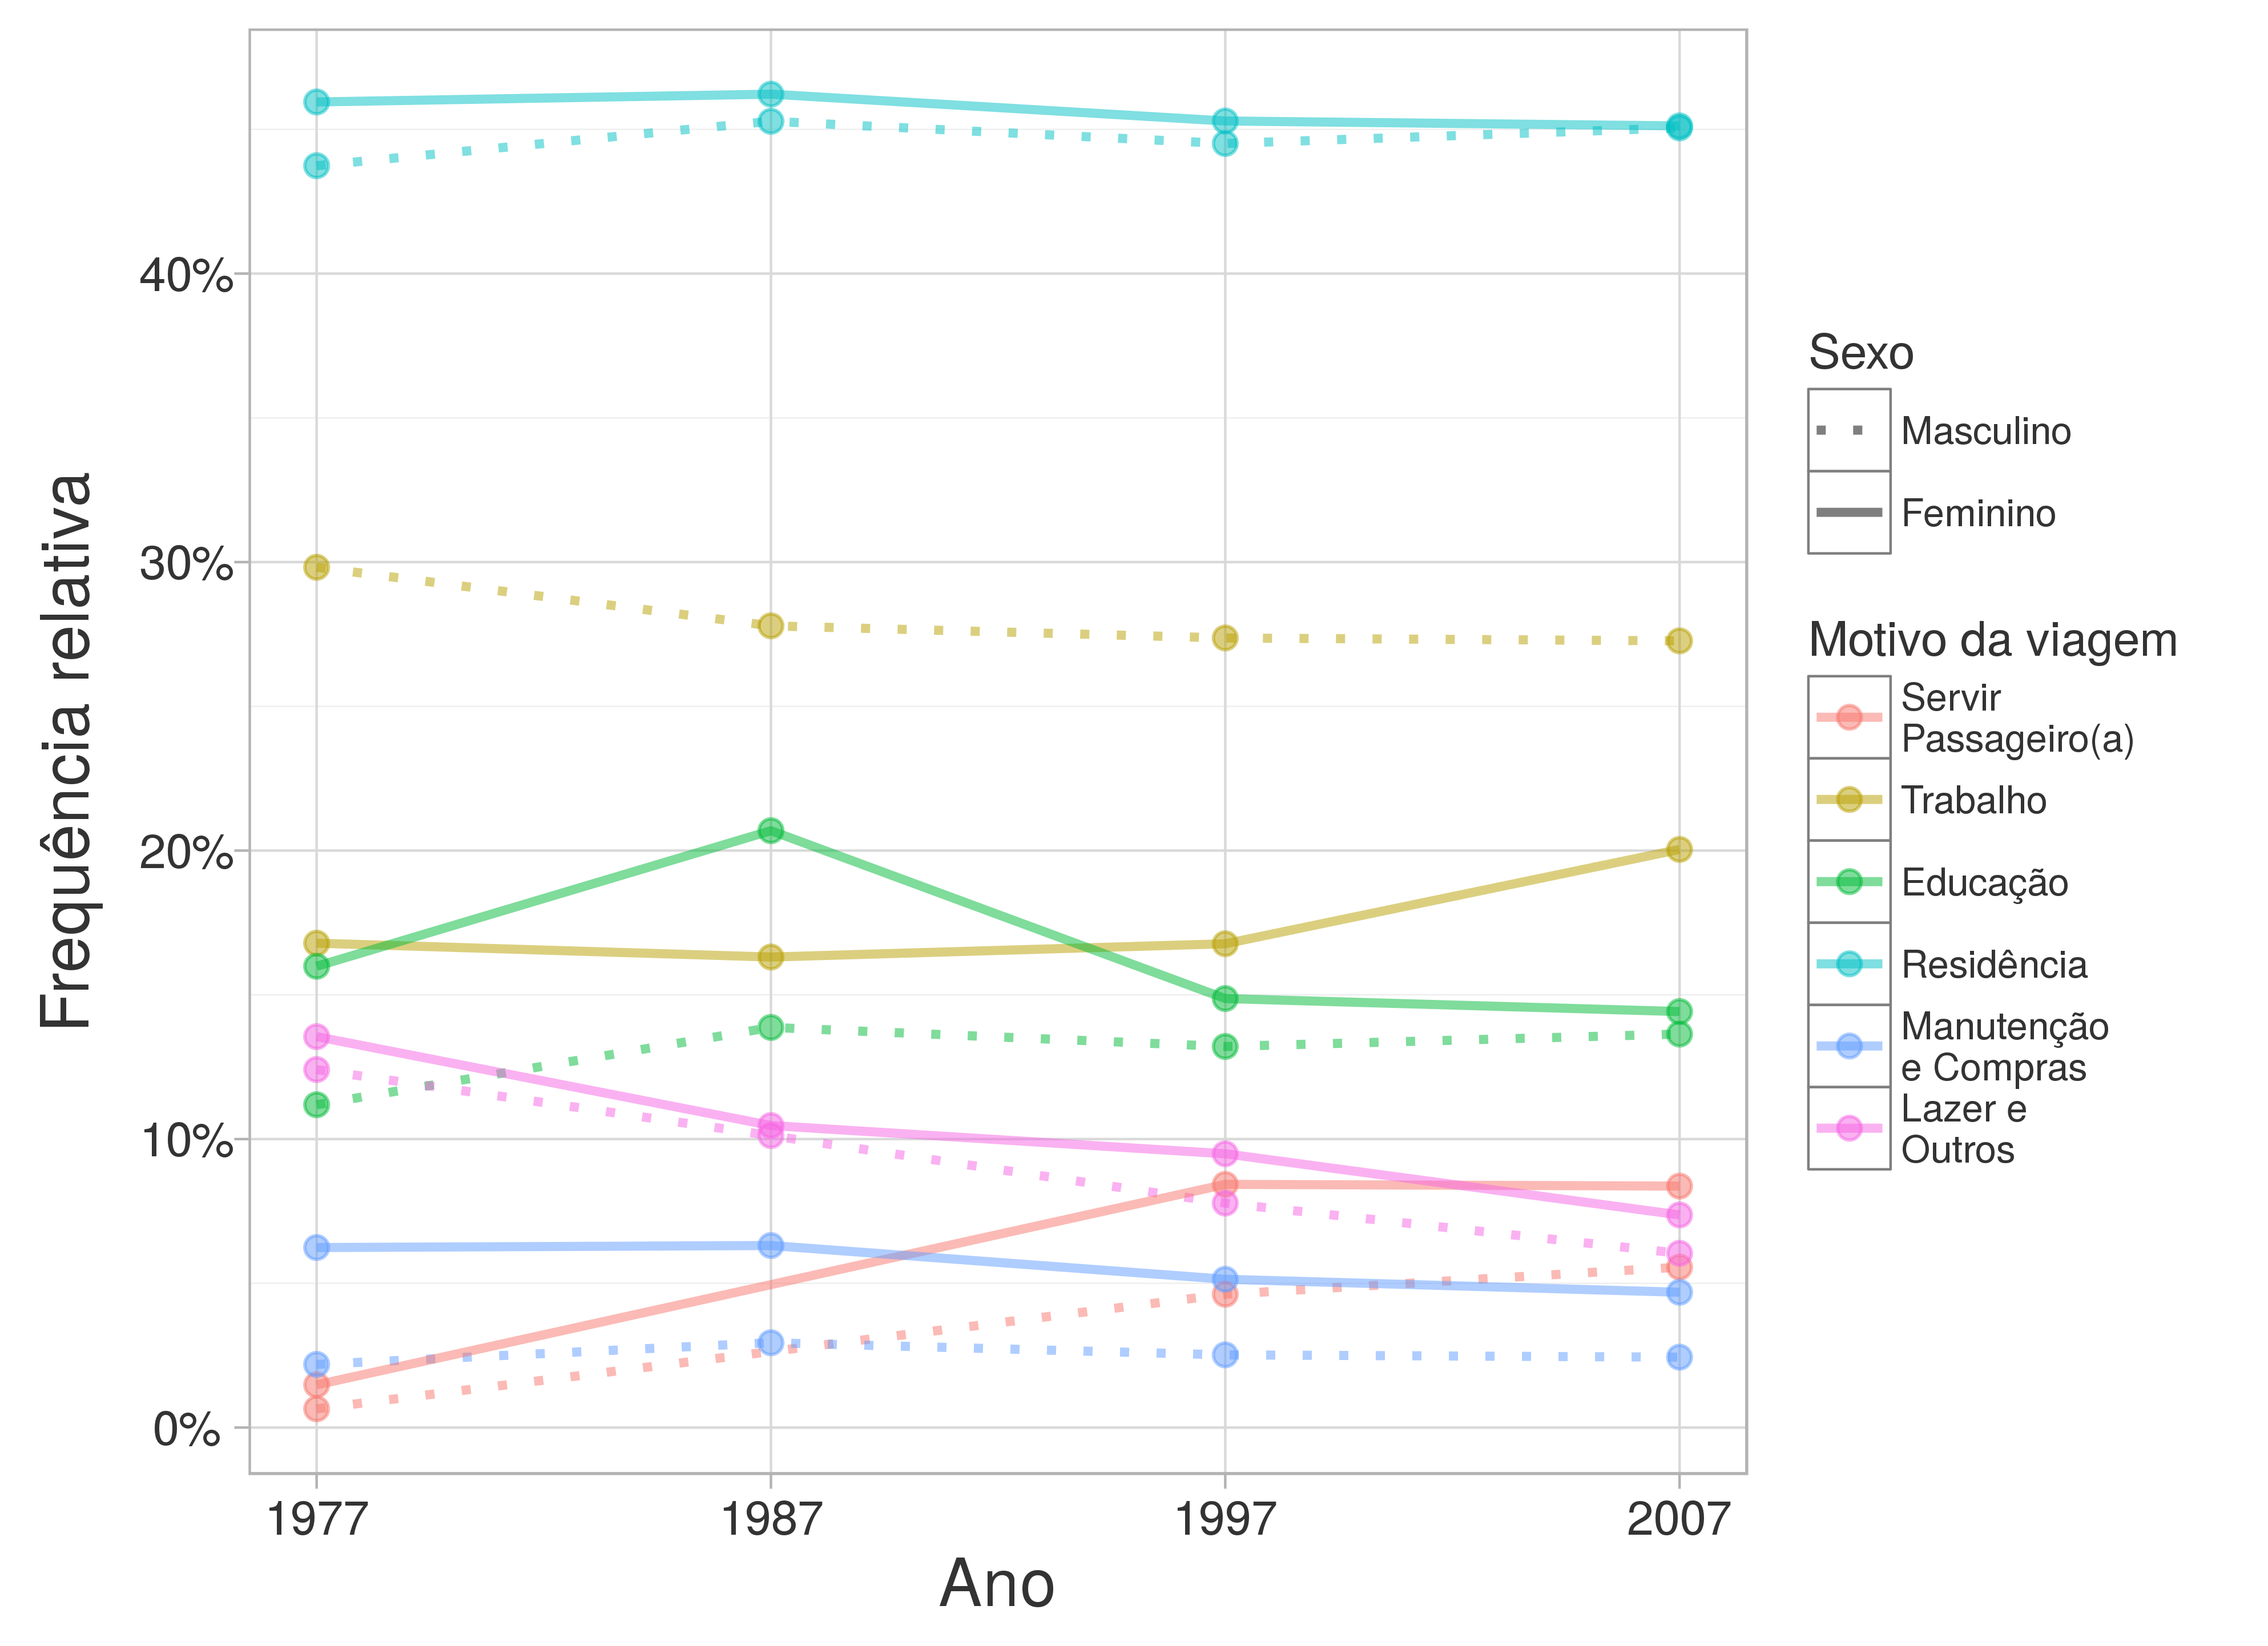
\includegraphics[width=0.9\textwidth]{./imagens/freq-motivo.png}%
    \end{center}%
%    \fonte{Compilação própria}
\end{grafico}%
% Estatísticas para registros com F_VIAG==1 e SEXO
% Expandido com FE_VIAG

%A variável \textbf{DURACAO} representa a duração total da viagem de uma pessoa, a duração média por pessoa é o somatório das durações dividido pelo número total de viagens de cada pessoa.
%Não existem \textit{missing values} neste campo, os valores mínimos para todos anos e ambos sexo são 0, bem como também são 0 os valores do primeiro quartil (25\%). Os valores das demais estatísticas (considerando os fatores de expansão para a população) estão apresentados na Tabela \ref{tab:estat-dur-med-viag}. Conforme já era de se esperar, para quem faz viagem no dia da pesquisa (número de viagem é não nulo) existe a predominância do valor 2, ou seja, são pessoas que saem de suas residências com um propósito único (trabalhar, estudar, fazer compras) e depois retornam à residência após a atividade.
%Percebe-se que, independente do sexo, o número médio de viagens por pessoa em relação a 1977 caiu um pouco em 1987 e 1997 (de 1,67 para 1,64) e subiu novamente em 2007 (para 1,70). Os desvios padrão caíram ao longo do tempo, indicando tendência de menor dispersão dos dados. Os valores de assimetria são positivos, indicando maior concentração à esquerda e cauda longa à direita da distribuição. Os valores de curtose evidenciam não tratar-se de distribuição normal.
%Analisando esses dados segmentados por sexo, vê-se que as medianas são iguais. O número médio e máximo de viagens para mulheres é sempre inferior ao dos homens, para o mesmo ano. Os valores de assimetria para o sexo feminino e o masculino são positivos e convergem para o valor geral com o passar das décadas. 
%A diferença entre o número médio de viagens de mulheres e homens vem diminuindo.

%\begin{table}[htb]
%\centering
%   \IBGEtab{%\renewcommand{\arraystretch}{1.5}%%\ABNTEXfontereduzida%
%        \renewcommand{\arraystretch}{1.5}
%        \caption{Estatísticas da variável ``PESS_DURACAO_MED'', por ano e por sexo}
%        \label{tab:estat-dur-med-viag}
%    }{%
%
%    \begin{tabular}{ccccccc}
%        \toprule
%        \textbf{Geral} & \multicolumn{3}{c}{\textbf{}} & \multicolumn{3}{c}{\textbf{}} \\ \hline
%        \textbf{ANO}   & \textbf{Média} & \textbf{Desvio Padrão} & \textbf{Mediana} & \textbf{Máximo} & \textbf{Assimetria} & \textbf{Curtose} \\ \midrule \midrule
%        \textbf{1977}  & 21,31 & 28,96 & 10,00 & 240 & 2,06 & 5,74 \\ \hline
%        \textbf{1987}  & 22,41 & 30,04 & 10,00 & 360 & 1,95 & 4,68 \\ \hline
%        \textbf{1997}  & 23,22 & 31,07 & 12,50 & 315 & 1,99 & 4,75 \\ \hline
%        \textbf{2007}  & 29,16 & 35,94 & 16,25 & 240 & 1,68 & 2,94 \\\bottomrule          
%
%        \textbf{Sexo Feminino} & \multicolumn{3}{c}{\textbf{}} & \multicolumn{3}{c}{\textbf{}} \\ \hline
%        \textbf{ANO}   & \textbf{Média} & \textbf{Desvio Padrão} & \textbf{Mediana} & \textbf{Máximo} & \textbf{Assimetria} & \textbf{Curtose} \\ \midrule \midrule
%        \textbf{1977}  & 16,49 & 25,70 &  5,00 & 240 & 1,80 & 4,41 \\ \hline
%        \textbf{1987}  & 17,55 & 26,68 &  5,00 & 360 & 1,66 & 3,16 \\ \hline
%        \textbf{1997}  & 19,89 & 28,67 & 10,00 & 300 & 1,82 & 3,93 \\ \hline
%        \textbf{2007}  & 26,49 & 34,93 & 15,00 & 240 & 1,55 & 2,45 \\\bottomrule
%        
%        \textbf{Sexo Masculino} & \multicolumn{3}{c}{\textbf{}} & \multicolumn{3}{c}{\textbf{}} \\ \hline
%        \textbf{ANO}   & \textbf{Média} & \textbf{Desvio Padrão} & \textbf{Mediana} & \textbf{Máximo} & \textbf{Assimetria} & \textbf{Curtose} \\ \midrule \midrule
%        \textbf{1977}  & 26,39 & 31,24 & 16,67 & 240 & 2,41 & 7,94 \\ \hline
%        \textbf{1987}  & 26,80 & 32,49 & 16,67 & 310 & 2,32 & 7,22 \\ \hline
%        \textbf{1997}  & 27,66 & 33,09 & 15,00 & 315 & 2,17 & 5,71 \\ \hline
%        \textbf{2007}  & 32,13 & 36,81 & 20,00 & 240 & 1,82 & 3,54 \\\bottomrule             
%       
%    \end{tabular}
%    }{%
%%		\fonte{Elaboração própria}
%	}
%\end{table}
%% Estatísticas para registros com F_PESS==1, filtro por SEXO
%% Expandido com FE_PESS
%
%\begin{table}[htb]
%\centering
%   \IBGEtab{%\renewcommand{\arraystretch}{1.5}%%\ABNTEXfontereduzida%
%        \renewcommand{\arraystretch}{1.5}
%        \caption{Estatísticas da variável ``PESS_DURACAO_MED'', por ano e por sexo, considerando somente quem fez viagem com duração superior a 4 minutos}
%        \label{tab:estat-dur-med-viag-maisde4}
%    }{%
%
%    \begin{tabular}{ccccccc}
%        \toprule
%        \textbf{Geral} & \multicolumn{3}{c}{\textbf{}} & \multicolumn{3}{c}{\textbf{}} \\ \hline
%        \textbf{ANO}   & \textbf{Média} & \textbf{Desvio Padrão} & \textbf{Mediana} & \textbf{Máximo} & \textbf{Assimetria} & \textbf{Curtose} \\ \midrule \midrule
%        \textbf{1977}  & 35,50 & 29,92 & 27,50 & 240 & 1,83 & 4,76 \\ \hline
%        \textbf{1987}  & 36,00 & 31,02 & 26,25 & 360 & 1,67 & 3,58 \\ \hline
%        \textbf{1997}  & 36,90 & 32,11 & 26,67 & 315 & 1,73 & 3,57 \\ \hline
%        \textbf{2007}  & 43,05 & 36,20 & 30,00 & 240 & 1,47 & 2,16 \\\bottomrule          
%
%        \textbf{Sexo Feminino} & \multicolumn{3}{c}{\textbf{}} & \multicolumn{3}{c}{\textbf{}} \\ \hline
%        \textbf{ANO}   & \textbf{Média} & \textbf{Desvio Padrão} & \textbf{Mediana} & \textbf{Máximo} & \textbf{Assimetria} & \textbf{Curtose} \\ \midrule \midrule
%        \textbf{1977}  & 32,39 & 28,00 & 23,33 & 235 & 1,97 & 5,64 \\ \hline
%        \textbf{1987}  & 33,48 & 28,88 & 22,50 & 360 & 1,88 & 5,10 \\ \hline
%        \textbf{1997}  & 34,48 & 30,39 & 25,00 & 300 & 1,82 & 3,90 \\ \hline
%        \textbf{2007}  & 41,79 & 35,87 & 30,00 & 240 & 1,53 & 2,37 \\\bottomrule
%        
%        \textbf{Sexo Masculino} & \multicolumn{3}{c}{\textbf{}} & \multicolumn{3}{c}{\textbf{}} \\ \hline
%        \textbf{ANO}   & \textbf{Média} & \textbf{Desvio Padrão} & \textbf{Mediana} & \textbf{Máximo} & \textbf{Assimetria} & \textbf{Curtose} \\ \midrule \midrule
%        \textbf{1977}  & 37,89 & 31,10 & 30,00 & 240 & 1,73 & 4,22 \\ \hline
%        \textbf{1987}  & 38,89 & 32,39 & 30,00 & 310 & 1,52 & 2,71 \\ \hline
%        \textbf{1997}  & 39,10 & 33,44 & 30,00 & 315 & 1,65 & 3,25 \\ \hline
%        \textbf{2007}  & 44,27 & 36,48 & 30,00 & 240 & 1,42 & 1,99 \\\bottomrule             
%       
%    \end{tabular}
%    }{%
%%		\fonte{Elaboração própria}
%	}
%\end{table}
%% Estatísticas para registros com F_PESS==1, filtro por SEXO
%% Expandido com FE_PESS

%\begin{grafico}[htb]%
%    \caption{\label{graf:distr-duracao}Distribuição da variável ``PESS_DURACAO_MED'' por ano e por sexo}%
%    \begin{center}%
%        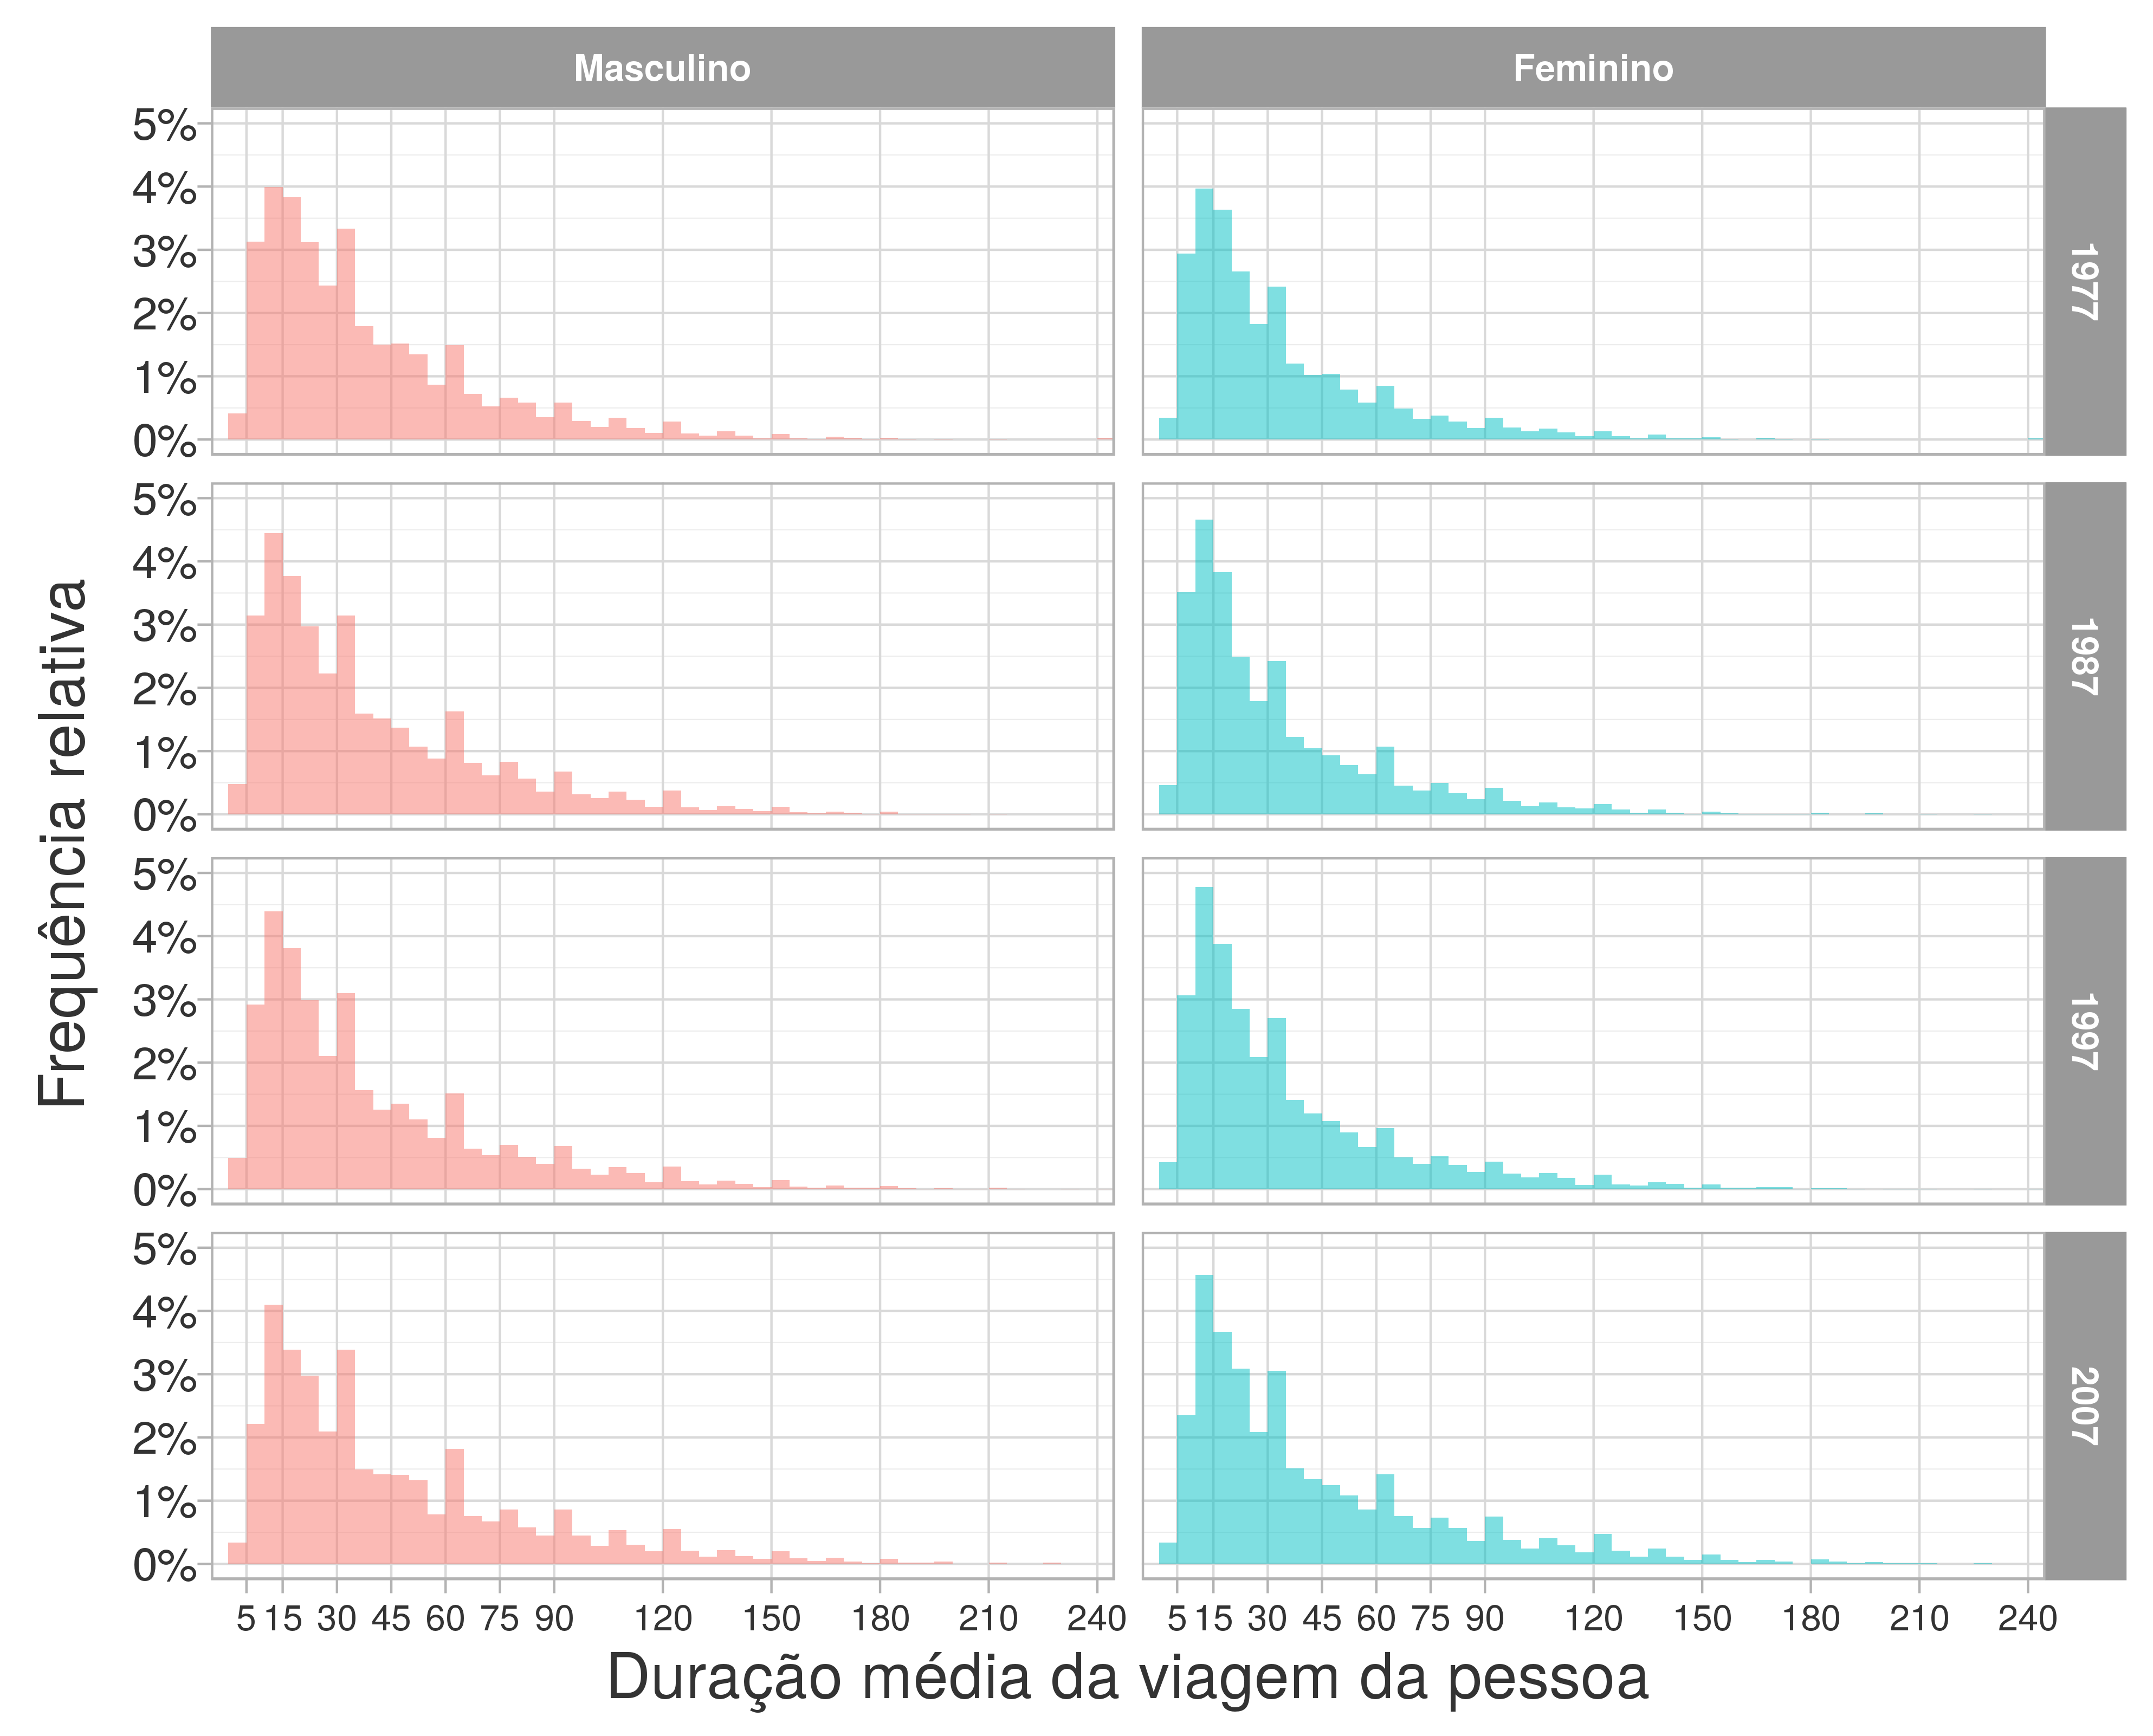
\includegraphics[width=1\textwidth]{./imagens/pess-duracao-med.png}%
%    \end{center}%
%%    \fonte{Compilação própria}
%\end{grafico}%
%% Estatísticas para registros com F_PESS==1 e SEXO
%% Expandido com FE_PESS

%\begin{table}[htb]
%\centering
%   \IBGEtab{%\renewcommand{\arraystretch}{1.5}%%\ABNTEXfontereduzida%
%        \renewcommand{\arraystretch}{1.5}
%        \caption{Estatísticas da variável ``FAM_DURACAO_TOT'', por ano}
%        \label{tab:estat-fam-duracao-tot}
%    }{%
%
%    \begin{tabular}{ccccccc}
%        \toprule
%        \textbf{} & \multicolumn{6}{c}{\textbf{Considerando famílias em que a duração média é superior a 4 minutos}} \\ \hline
%        \textbf{ANO}   & \textbf{Média} & \textbf{Desvio Padrão} & \textbf{Mediana} & \textbf{Máximo} & \textbf{Assimetria} & \textbf{Curtose} \\ \midrule \midrule
%        \textbf{1977}  & 293,14 & 222,68 & 240,00 & 2090 & 1,59 & 3,87 \\ \hline
%        \textbf{1987}  & 265,22 & 199,68 & 220,00 & 2703 & 1,69 & 5,23 \\ \hline
%        \textbf{1997}  & 256,91 & 187,29 & 215,00 & 1890 & 1,42 & 2,87 \\ \hline
%        \textbf{2007}  & 279,18 & 201,34 & 240,00 & 3035 & 1,72 & 9,02 \\\bottomrule          
%
%        \textbf{} & \multicolumn{6}{c}{\textbf{Considerando inclusive família em que ninguém fez viagem}} \\ \hline
%        \textbf{ANO}   & \textbf{Média} & \textbf{Desvio Padrão} & \textbf{Mediana} & \textbf{Máximo} & \textbf{Assimetria} & \textbf{Curtose} \\ \midrule \midrule
%        \textbf{1977}  & 270,74 & 220,08 & 220,00 & 2090 & 1,55 & 3,86 \\ \hline
%        \textbf{1987}  & 251,07 & 200,59 & 210,00 & 2703 & 1,68 & 5,71 \\ \hline
%        \textbf{1997}  & 240,13 & 193,64 & 200,00 & 1890 & 1,37 & 2,87 \\ \hline
%        \textbf{2007}  & 242,07 & 194,09 & 205,00 & 3035 & 1,58 & 7,25 \\\bottomrule
%
%    \end{tabular}
%    }{%
%%		\fonte{Elaboração própria}
%	}
%\end{table}
%% Estatísticas para registros com F_FAM==1, filtro por ANO
%% Expandido com FE_FAM

%O Gráfico \ref{graf:distr-dur-viag} foi construído considerando-se apenas as viagens cuja duração fosse igual ou superior a 5 minutos. Em todos os anos, para homens e para mulheres, percebem-se alguns picos que ocorrem nos valores múltiplos de cinco minutos. Isso porque a duração de viagem é aquela percebida e declarada pelo(a) respondente. Em 1977, a duração das viagens mais curtas (como 5 e 30 minutos) era menos frequente entre as mulheres (13\% e 14\%, respectivamente) do que entre os homens (26\% e 15\%). Em 1987 as viagens de 5 minutos passam a ser mais frequentes entre mulheres (32\%) do que entre homens (26,5\%). Essa situação se inverte em 1997 e retorna em 2007.
%Em todos os anos as viagens mais longas (de 60 e 90 minutos) são mais frequentes entre os homens do que entre as mulheres.
%Na Tabela \ref{tab:dur-med-viag} são apresentadas as durações médias de viagens para homens e mulheres. As médias de homens são superiores às das mulheres, ao nível de significância estatística de 5\%. É possível perceber que a duração média de viagem para ambos vem crescendo e a diferença entre esses grupos vem diminuindo.


A variável \textbf{DURACAO} tem suas principais estatísticas apresentadas na Tabela \ref{tab:estat-duracao}.
Não existem \textit{missing values} neste campo e, desconsiderando quem não fez viagem (duração igual a 0 minutos), os valores mínimos para todos anos e ambos sexo são 1 minuto.
As medianas da duração, independente do sexo, saem de 30 minutos em 1977 para 20 minutos em 1987 e 1997 e retornam para o valor 30 em 2007.
Os valores de assimetria são todos positivos, indicando maior concentração à esquerda e cauda longa à direita da distribuição.
Os valores de curtose evidenciam não se tratar de distribuição normal.
O tempo médio geral de viagem vai de 1977 para 1987 e daí em diante só aumenta, comportamento semelhante ao segmento feminino.
Os tempos médios das viagens do homens cresce sistematicamente década a década, da ordem de 1 minuto entre 1977, 1987 e 1997. Já 2007 o acréscimo no tempo médio de viagem masculino subiu 4,5 minutos - tal efeito pode ser explicado pela expansão urbana da RMSP.
Analisando esses dados segmentados por sexo, vê-se que as medianas das mulheres são sempre 5 minutos a menos que as dos homens. 
A diferença entre as durações médias das viagens de mulheres e de homens cresce de quase 0,5 minuto em 1977 para pouco mais de 5,5 minutos em 1987 e vem diminuindo desde então.
Foram feitos teste t para avaliar se eram estatisticamente significantes (intervalo de confiança de 95\%) as médias entre os sexos, no mesmo ano; e entre os anos, para o mesmo sexo. Todas médias foram estatisticamente diferentes umas das outras.

\begin{table}[htb]
\centering
   \IBGEtab{%\renewcommand{\arraystretch}{1.5}%%\ABNTEXfontereduzida%
        \renewcommand{\arraystretch}{1.5}
        \caption{Estatísticas da variável ``DURACAO'', por ano}
        \label{tab:estat-duracao}
    }{%

    \begin{tabular}{ccccccc}
        \toprule
        \textbf{Total} & \multicolumn{6}{c}{\textbf{}} \\ \hline
        \textbf{ANO}   & \textbf{Média} & \textbf{Desvio Padrão} & \textbf{Mediana} & \textbf{Máximo} & \textbf{Assimetria} & \textbf{Curtose} \\ \midrule \midrule
        \textbf{1977}  & 36,07 & 31,99 & 30 & 240 & 1,74 & 3,78 \\ \hline
        \textbf{1987}  & 33,27 & 31,99 & 20 & 360 & 1,92 & 4,97 \\ \hline
        \textbf{1997}  & 34,13 & 33,52 & 20 & 370 & 1,94 & 4,54 \\ \hline
        \textbf{2007}  & 39,29 & 37,22 & 30 & 299 & 1,74 & 3,37 \\\bottomrule          

        \textbf{Sexo feminino} & \multicolumn{6}{c}{\textbf{}} \\ \hline
        \textbf{ANO}   & \textbf{Média} & \textbf{Desvio Padrão} & \textbf{Mediana} & \textbf{Máximo} & \textbf{Assimetria} & \textbf{Curtose} \\ \midrule \midrule
        \textbf{1977}  & 34,09 & 30,54 & 25 & 240 & 1,81 & 4,12 \\ \hline
        \textbf{1987}  & 30,15 & 29,76 & 20 & 360 & 2,08 & 5,89 \\ \hline
        \textbf{1997}  & 31,97 & 31,67 & 20 & 315 & 2,02 & 4,78 \\ \hline
        \textbf{2007}  & 37,96 & 36,72 & 25 & 299 & 1,81 & 3,68 \\\bottomrule     

        \textbf{Sexo Masculino} & \multicolumn{6}{c}{\textbf{}} \\ \hline
        \textbf{ANO}   & \textbf{Média} & \textbf{Desvio Padrão} & \textbf{Mediana} & \textbf{Máximo} & \textbf{Assimetria} & \textbf{Curtose} \\ \midrule \midrule
        \textbf{1977}  & 34,47 & 32,89 & 30 & 240 & 1,69 & 3,53 \\ \hline
        \textbf{1987}  & 35,83 & 33,50 & 25 & 360 & 1,80 & 4,36 \\ \hline
        \textbf{1997}  & 36,11 & 35,02 & 25 & 370 & 1,86 & 4,25 \\ \hline
        \textbf{2007}  & 40,61 & 37,67 & 30 & 270 & 1,67 & 3,11 \\\bottomrule             

    \end{tabular}
    }{%
%		\fonte{Elaboração própria}
	}
\end{table}
% Estatísticas para registros com F_FAM==1, filtro por ANO
% Expandido com FE_FAM

Com o intuito de melhor explorar as durações médias das viagens analisando modos e motivos, foram elaborados os Gráficos \ref{graf:duracao-modo}, \ref{graf:duracao-coletivo} e \ref{graf:duracao-motivo}.
O Gráfico \ref{graf:duracao-modo} apresenta as durações médias do transporte coletivo, individual e a pé, para homens e para mulheres. Verifica-se que:
\begin{compactitem}[]
\item (i) As durações médias de homens e mulheres são muito próximas para as viagens a pé, girando em torno de 15 minutos para ambos.
\item (ii) A duração média no transporte individual cai um pouco de 1977 para 1987 (de 23,0 para 20,4 min para mulheres e de 27,07 para 25,7 min para homens).
\item (iii) A duração média no transporte individual aumenta de 1987 para 2007 (7,3 min para mulheres e 8,1 min para homens).
\item (iv) A duração média no transporte coletivo aumenta entre 1977 e 2007 para ambos sexos, sendo a taxa mais acentuada de 1997 para 2007. 
\item (v) As diferenças nas durações médias nas viagens feitas por transporte coletivo entre mulheres e homens aumenta de 1977 (4,2 min) para 1987 (6,3 min) e depois decresce nas décadas seguintes (6,0 min em 1997 e 3,2 min em 2007).
\end{compactitem}

\begin{grafico}[htb]%
    \caption{\label{graf:duracao-modo}Comparação entre as durações médias de viagem por ano e por sexo, segundo os modos (agregados)}%
    \begin{center}%
        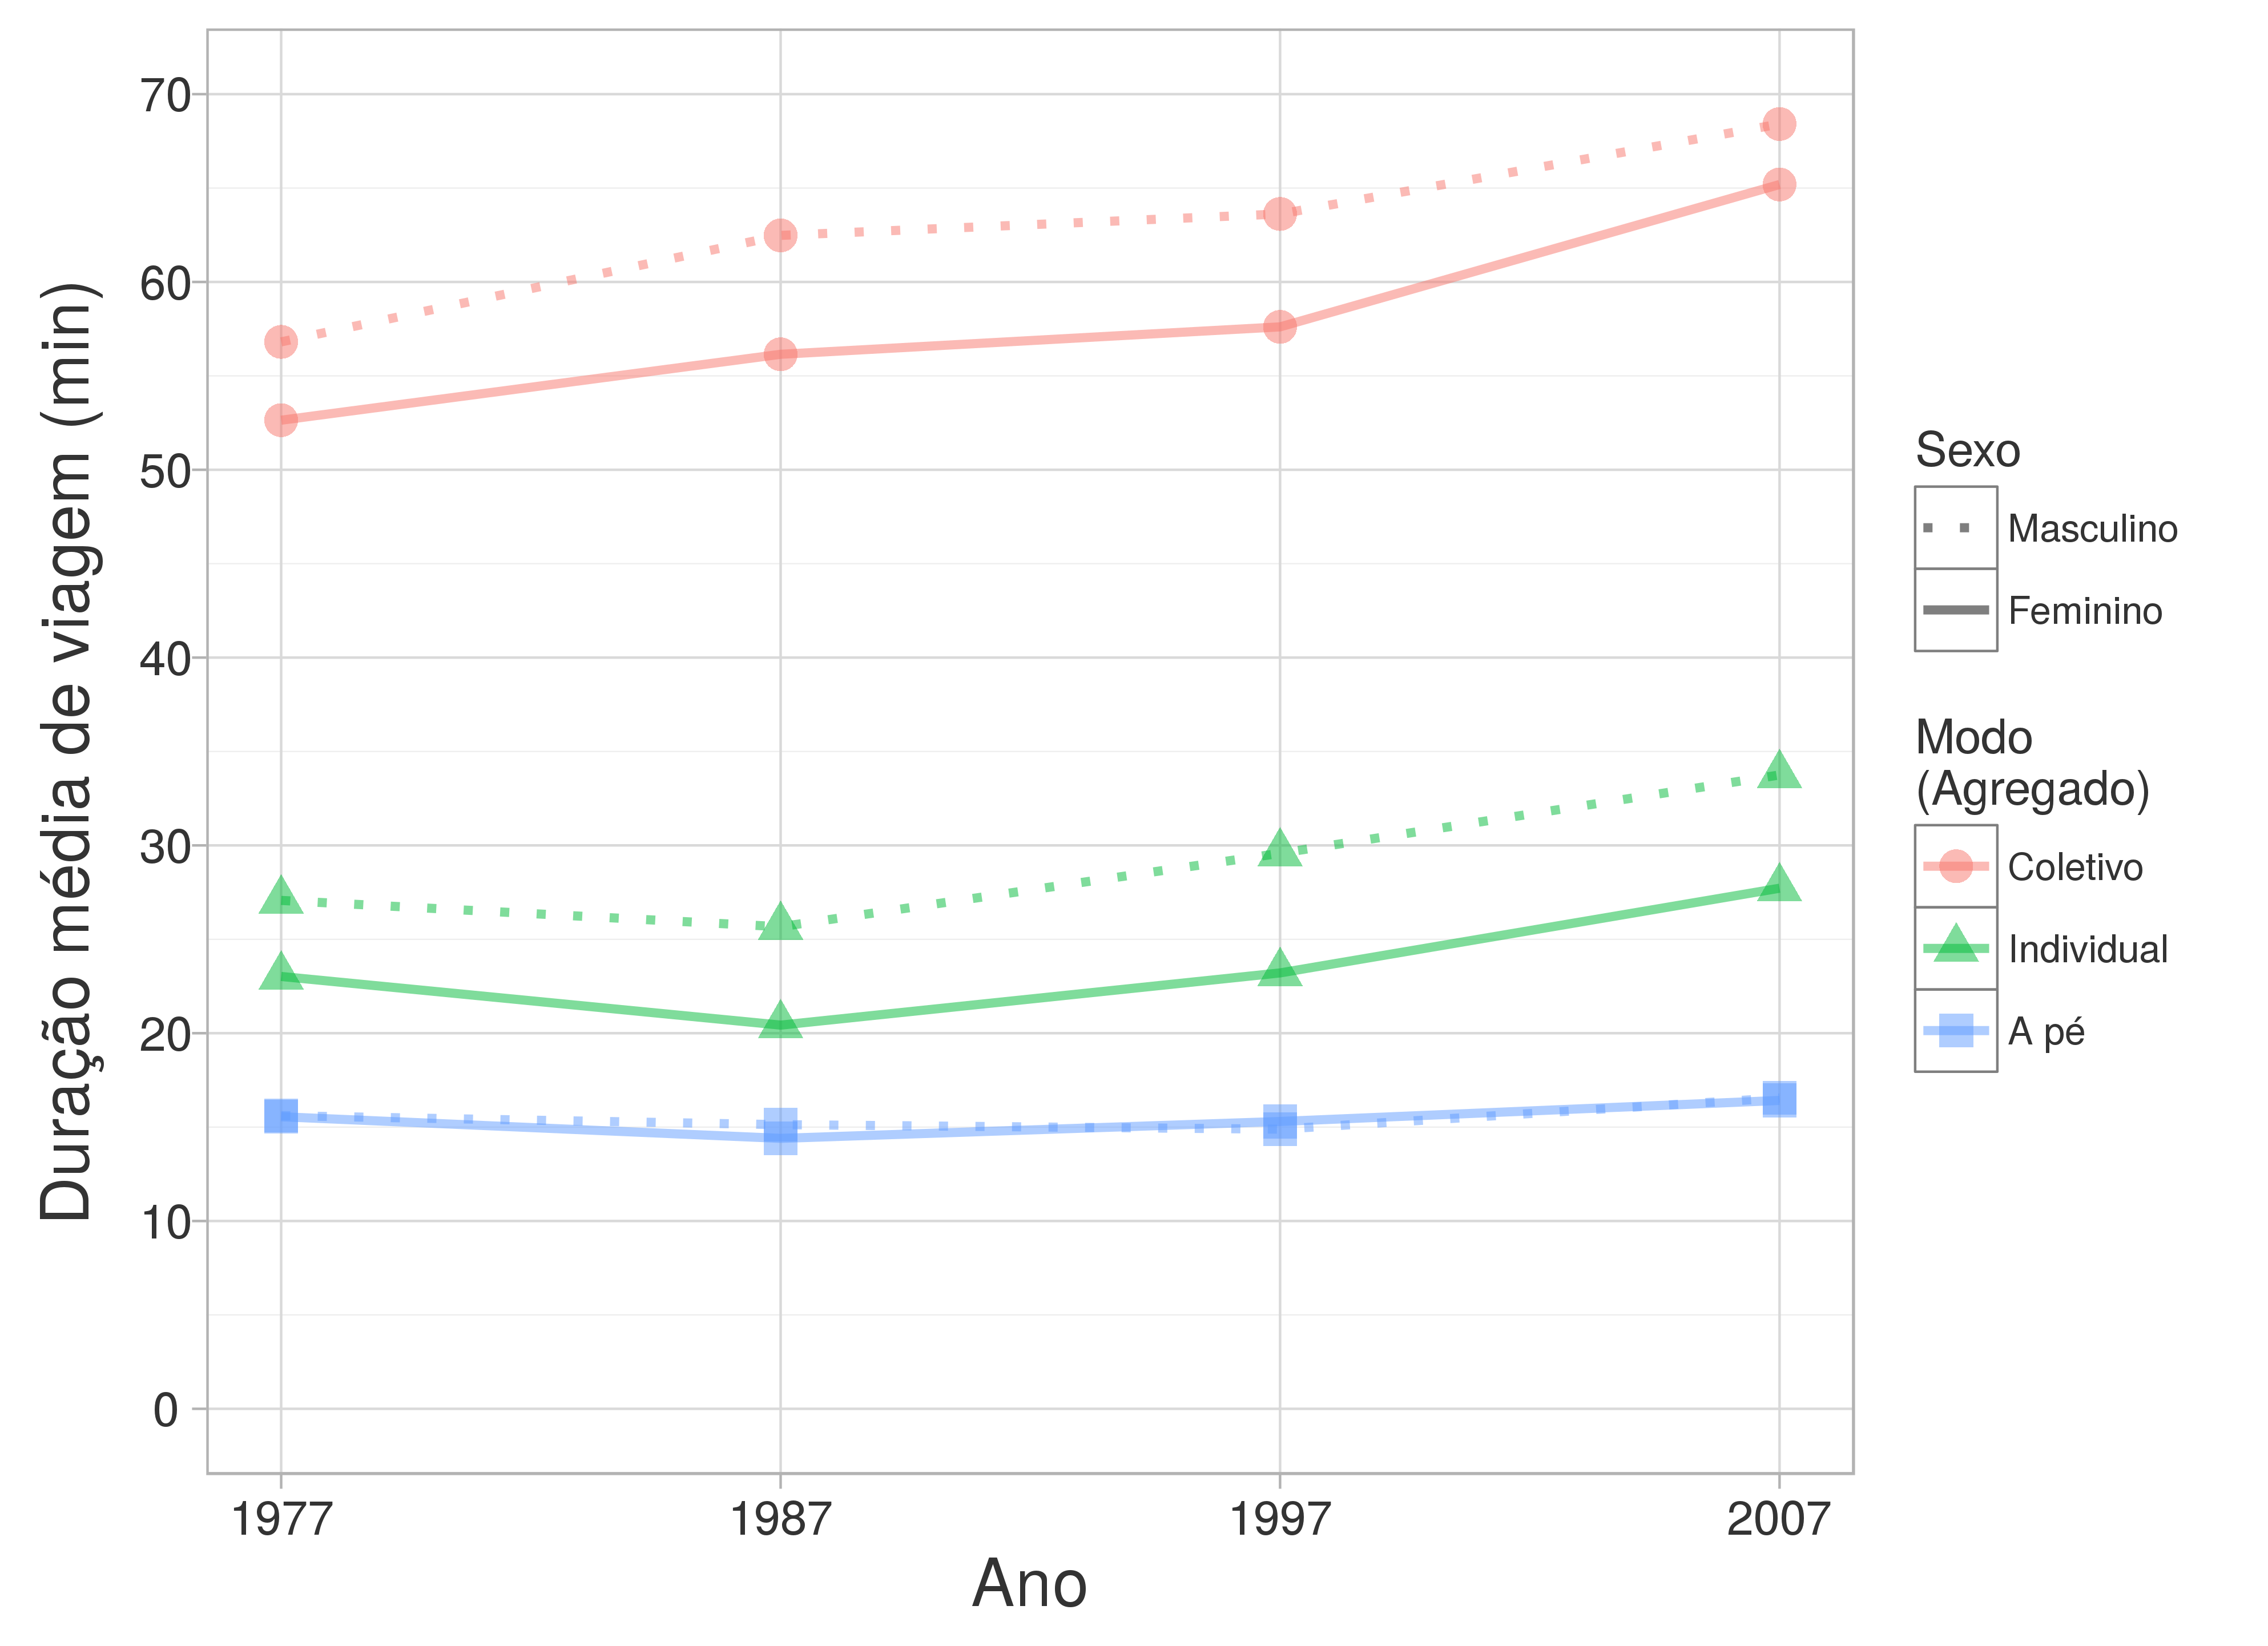
\includegraphics[width=1\textwidth]{./imagens/duracao-modo.png}%
    \end{center}%
%    \fonte{Compilação própria}
\end{grafico}%
% Estatísticas para registros com F_VIAG==1 e SEXO
% Expandido com FE_VIAG

O Gráfico \ref{graf:duracao-coletivo} apresenta as durações médias dos modos de transporte coletivo (ônibus de linha, ônibus de empresa/escolar, lotação/perua/van/microônibus, Metrô e trem), para homens e para mulheres - foram separados os modos de alta capacidade dos demais para facilitar a compreensão dos gráficos. Verifica-se que:
\begin{compactitem}[]
\item (i) A duração média do trem é superior a todos outros modos, inclusive o Metrô, com médias gerais caindo de 83,3 min em 1977 para 80,8 min em 1987 e crescendo para 89,45 min em 1997. Em 2007, esse valor permanece no mesmo patamar de 1997 (90,2 min).
\item (ii) Para o trem, a duração média feminina é inferior à masculina em 1977 (diferença de 2,9 min) e 1987 (diferença de 2,1 min), supera a masculina em 1997 (por 1,6 min) e distancia da masculina em 2007 (diferença de 8,0 min).
\item (iii) A duração média das viagens de Metrô crescem sistematicamente, pelo menos 6 min por década, de 1977 (53,8 min) a 2007 (74,4 min).
\item (iv) Para o Metrô, a duração média feminina é superior à masculina em 1977 (diferença de 1,3 min) e em 2007 (diferença de 1,7 min). A situação é inversa, com durações médias das viagens masculinas superiores às femininas em 1987 (diferença de 3,8 min) e 1997 (diferença de 5,0 min).
\item (v) A duração média das viagens dos ônibus de linha crescem sistematicamente, 5 min por década entre 1977 e 1987, 0,9 min entre 1987 e 1997, e 8,8 min entre 1997 e 2007.
\item (vi) Para ônibus de linha, a duração média feminina é inferior à masculina - a diferença é de 4,0 min em 1977, de 6,9 min em 1987, de 6,3 min em 1997 e de 3,9 min em 2007.
\item (vii) A duração média das viagens de lotações/vans crescem de 1977 (54,1 min) para 1987 (60,8 min), caem em 1997 (49,9 min) e sobem novamente em 2007 (66,3 min).
\item (viii) Para viagens de lotações/vans, a duração média feminina era inferior à masculina em 1977 (diferença de 6,4 min) e em 2007 (diferença 9,4 de min). A situação é inversa em 1987, com diferenças de 7,7 min entre os sexos. E, em 1997, as durações médias são estatisticamente iguais.
\item (ix) A duração média das viagens de ônibus escolar/fretado são as menores entre os transportes coletivos, para ambos sexos variando numa faixa de 40,9 a 44,1 min.
\item (x) Para viagens de ônibus escolar/fretado, a duração média feminina é sempre inferior à masculina - a diferença é de 6,8 min em 1977, de 7,2 min em 1987, de 7,1 min em 1997 e de 2,9 min em 2007.
\end{compactitem}

\begin{grafico}[htb]%
    \caption{\label{graf:duracao-coletivo}Comparação entre as durações médias de viagem por ano e por sexo, segundo os modos coletivos}%
    \begin{center}%
        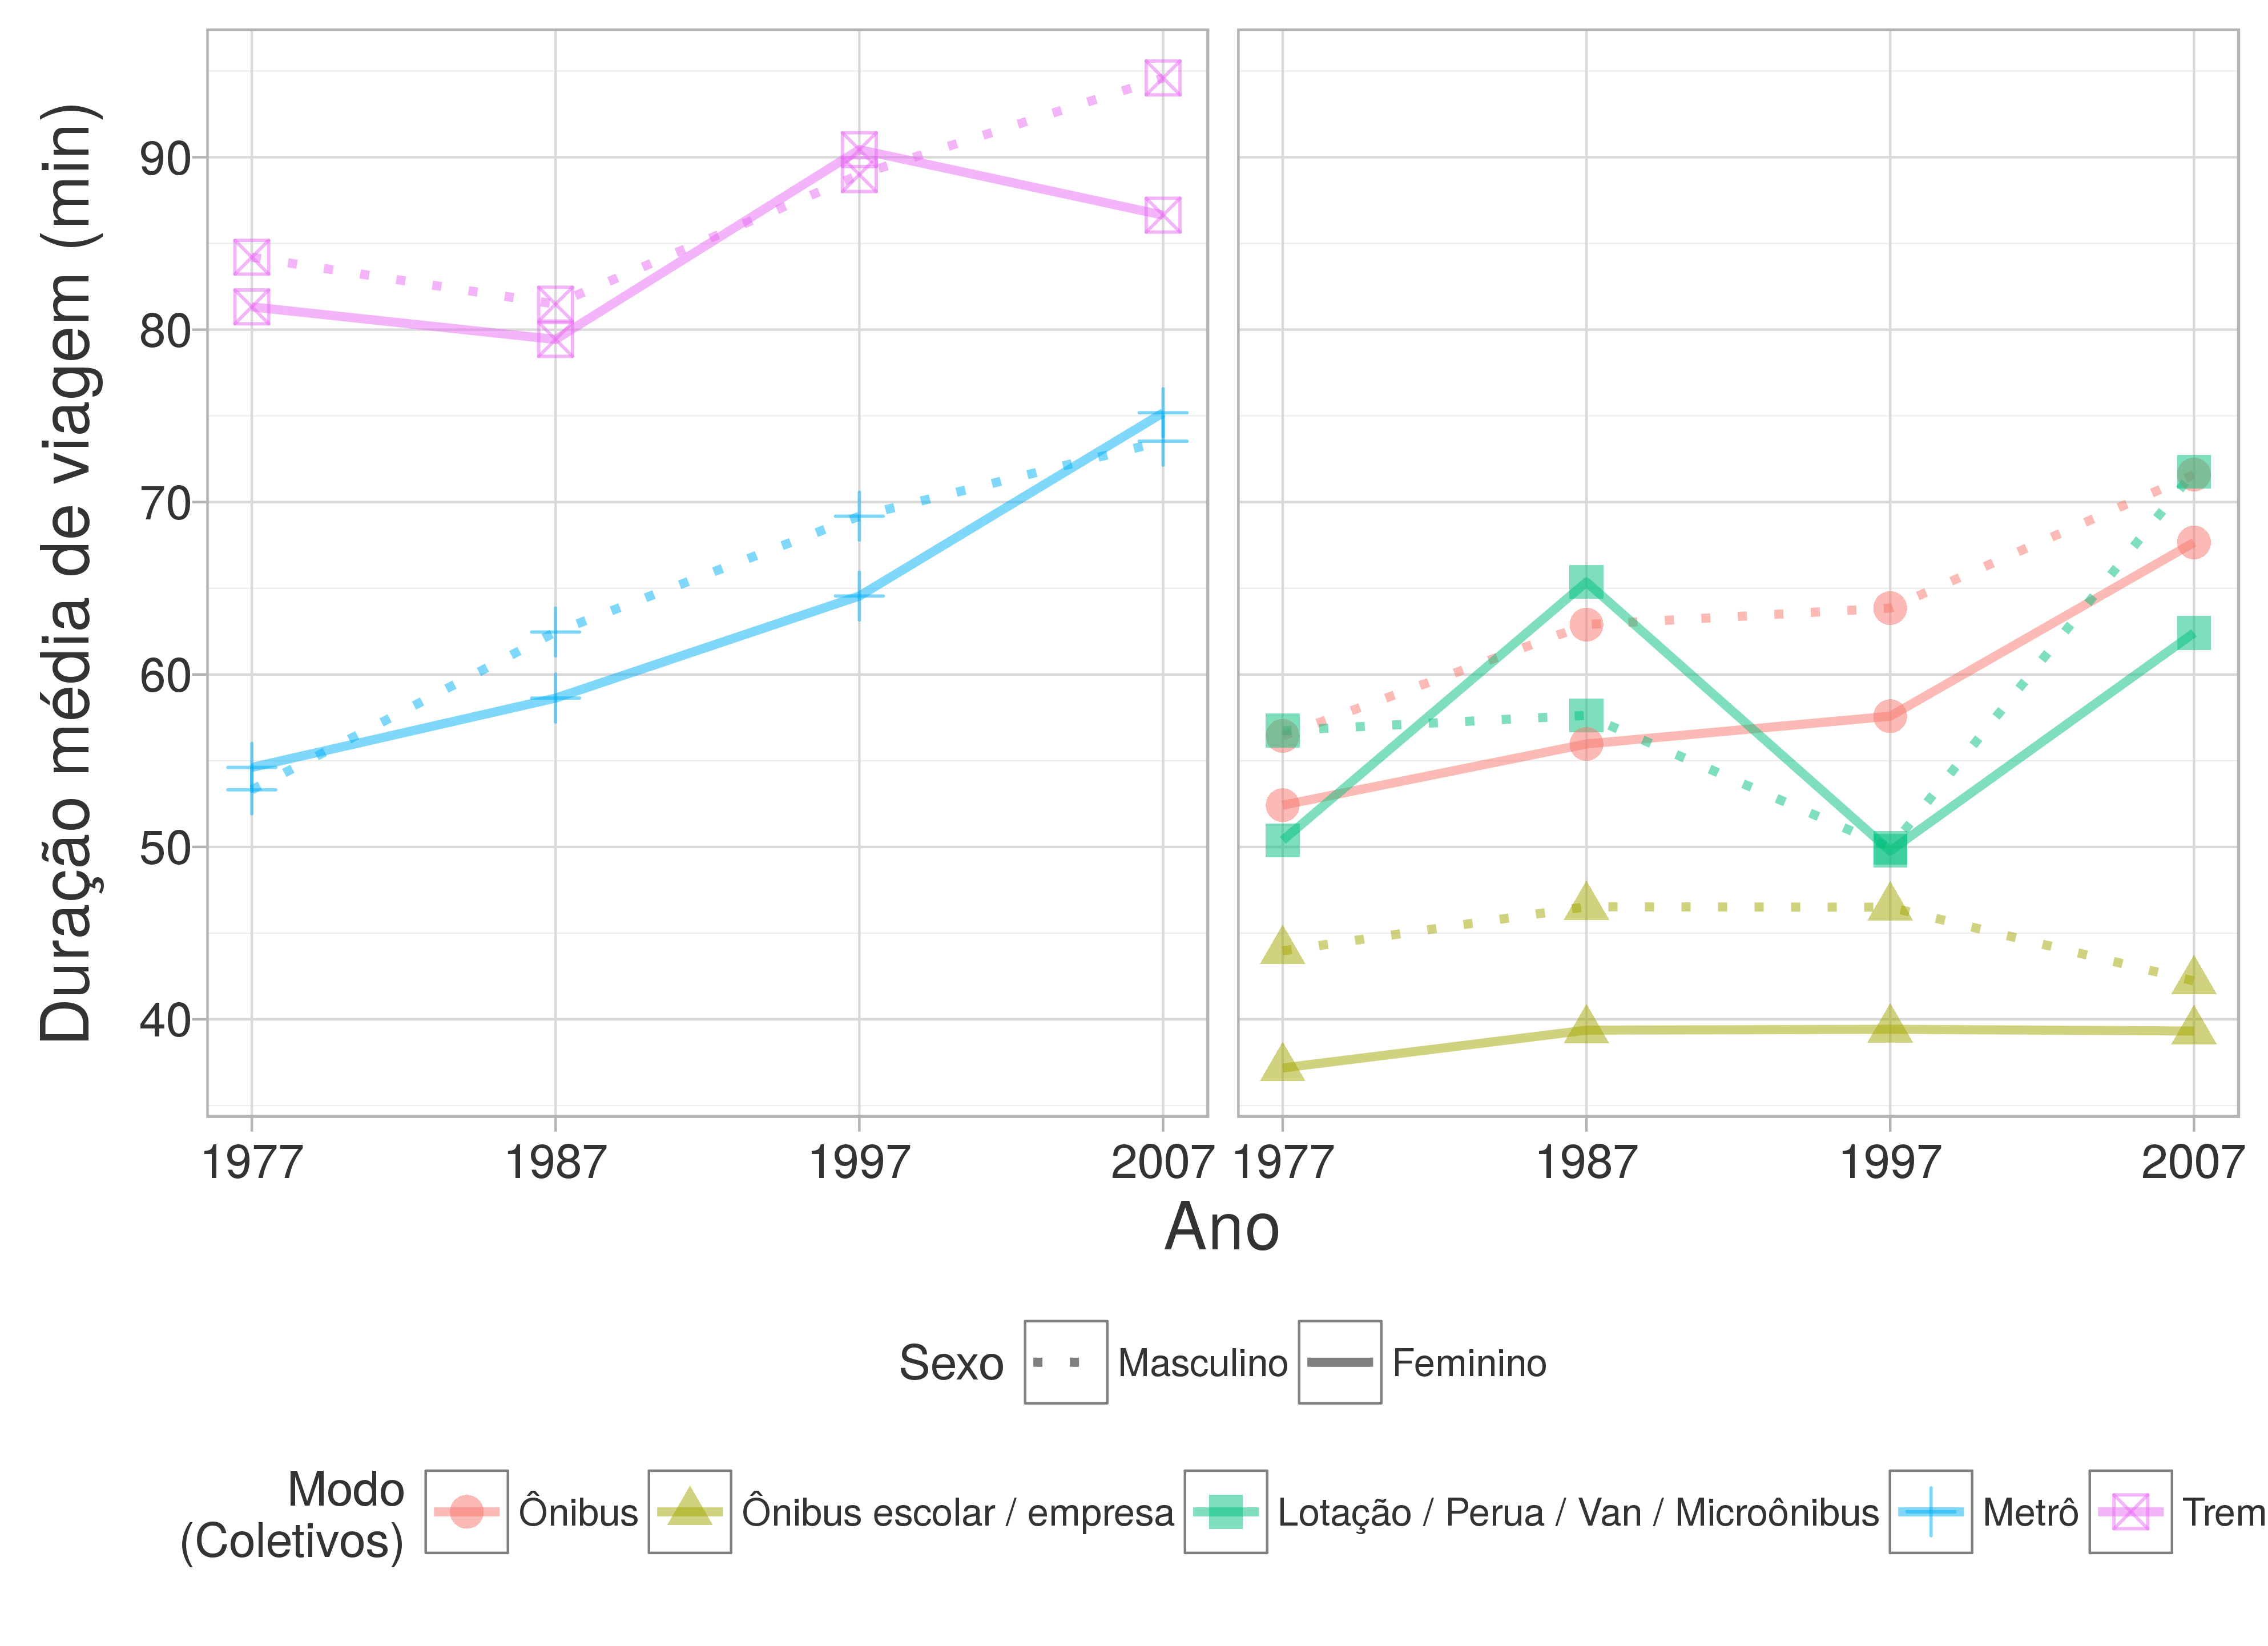
\includegraphics[width=1\textwidth]{./imagens/duracao-coletivo.png}%
    \end{center}%
%    \fonte{Compilação própria}
\end{grafico}%
% Estatísticas para registros com F_VIAG==1 e SEXO
% Expandido com FE_VIAG

O Gráfico \ref{graf:duracao-motivo} apresenta as durações médias por motivo de viagem (trabalho, educação, servir passageiro, manutenção/compras e lazer/outros), para homens e para mulheres. Verifica-se que:
\begin{compactitem}[]
\item (i) A duração média da viagem motivo trabalho (de natureza compulsória) é superior a de todos outros motivos. Ela permanece no mesmo patamar entre 1977 (40,9 min) e 1987 (40,8 min), sobe um pouco em 1997 (42,7 min) e continua a subir em 2007 (48,9 min).
\item (ii) Para o motivo trabalho, a duração média feminina é estatisticamente igual à masculina em 1977, inferior, em 1987 (diferença de 2,5 min) e em 1997 (diferenças de 1,3 min) e levemente superior em 2007 (0,7 min).
\item (iii) A duração média das viagens motivo educação decresce de 1977 (21,0 min) para 1987 (18,3 min), a partir de quando sobem até 2007 (26,1 min).
\item (iv) Para o motivo educação, a duração média feminina é praticamente igual à masculina em 1977 e em 1997 (diferenças de menos de 0,5 min), levemente inferior à masculina em 1987 (diferença de 0,9 min) e superior em 2007 (diferença de 0,6 min).
\item (v) A duração média das viagens motivo manutenção/compras decresce de 1977 (35,2 min) para 1987 (33,9 min), a partir de quando sobem até 2007 (38,0 min).
\item (vi) Para viagens motivo manutenção/compras, a duração média feminina é inferior à masculina - a diferença é de 1,9 min em 1977, de 0,7 min em 1987, de 3,3 min em 1997 e de 0,7 min em 2007.
\item (vii) A duração média das viagens motivo lazer/outros decresce de 1977 (37,5 min) para 1987 (34,7 min), a partir de quando sobem até 2007 (40,7 min).
\item (viii) Para viagens motivo lazer/outros, a duração média feminina é inferior à masculina - a diferença é de 3,3 min em 1977, de 5,6 min em 1987, de 4,0 min em 1997 e de 2,7 min em 2007.
\item (ix) A duração média das viagens motivo servir passageiro decresce de 1977 (37,2 min) para 1997 (20,43 min), a partir de quando sobem até 2007 (23,1 min). Vale destacar que em 1987 não havia o modo servir passageiro.
\item (x) Para viagens motivo servir passageiro,  a duração média feminina é estatisticamente igual à masculina em 1977, e inferior em 1997 (diferenças de 1,6 min) e em 2007 (diferenças de 2,7 min).
\end{compactitem}


\begin{grafico}[htb]%
    \caption{\label{graf:duracao-motivo}Comparação entre as durações médias de viagem por ano e por sexo, segundo o motivo da viagem}%
    \begin{center}%
        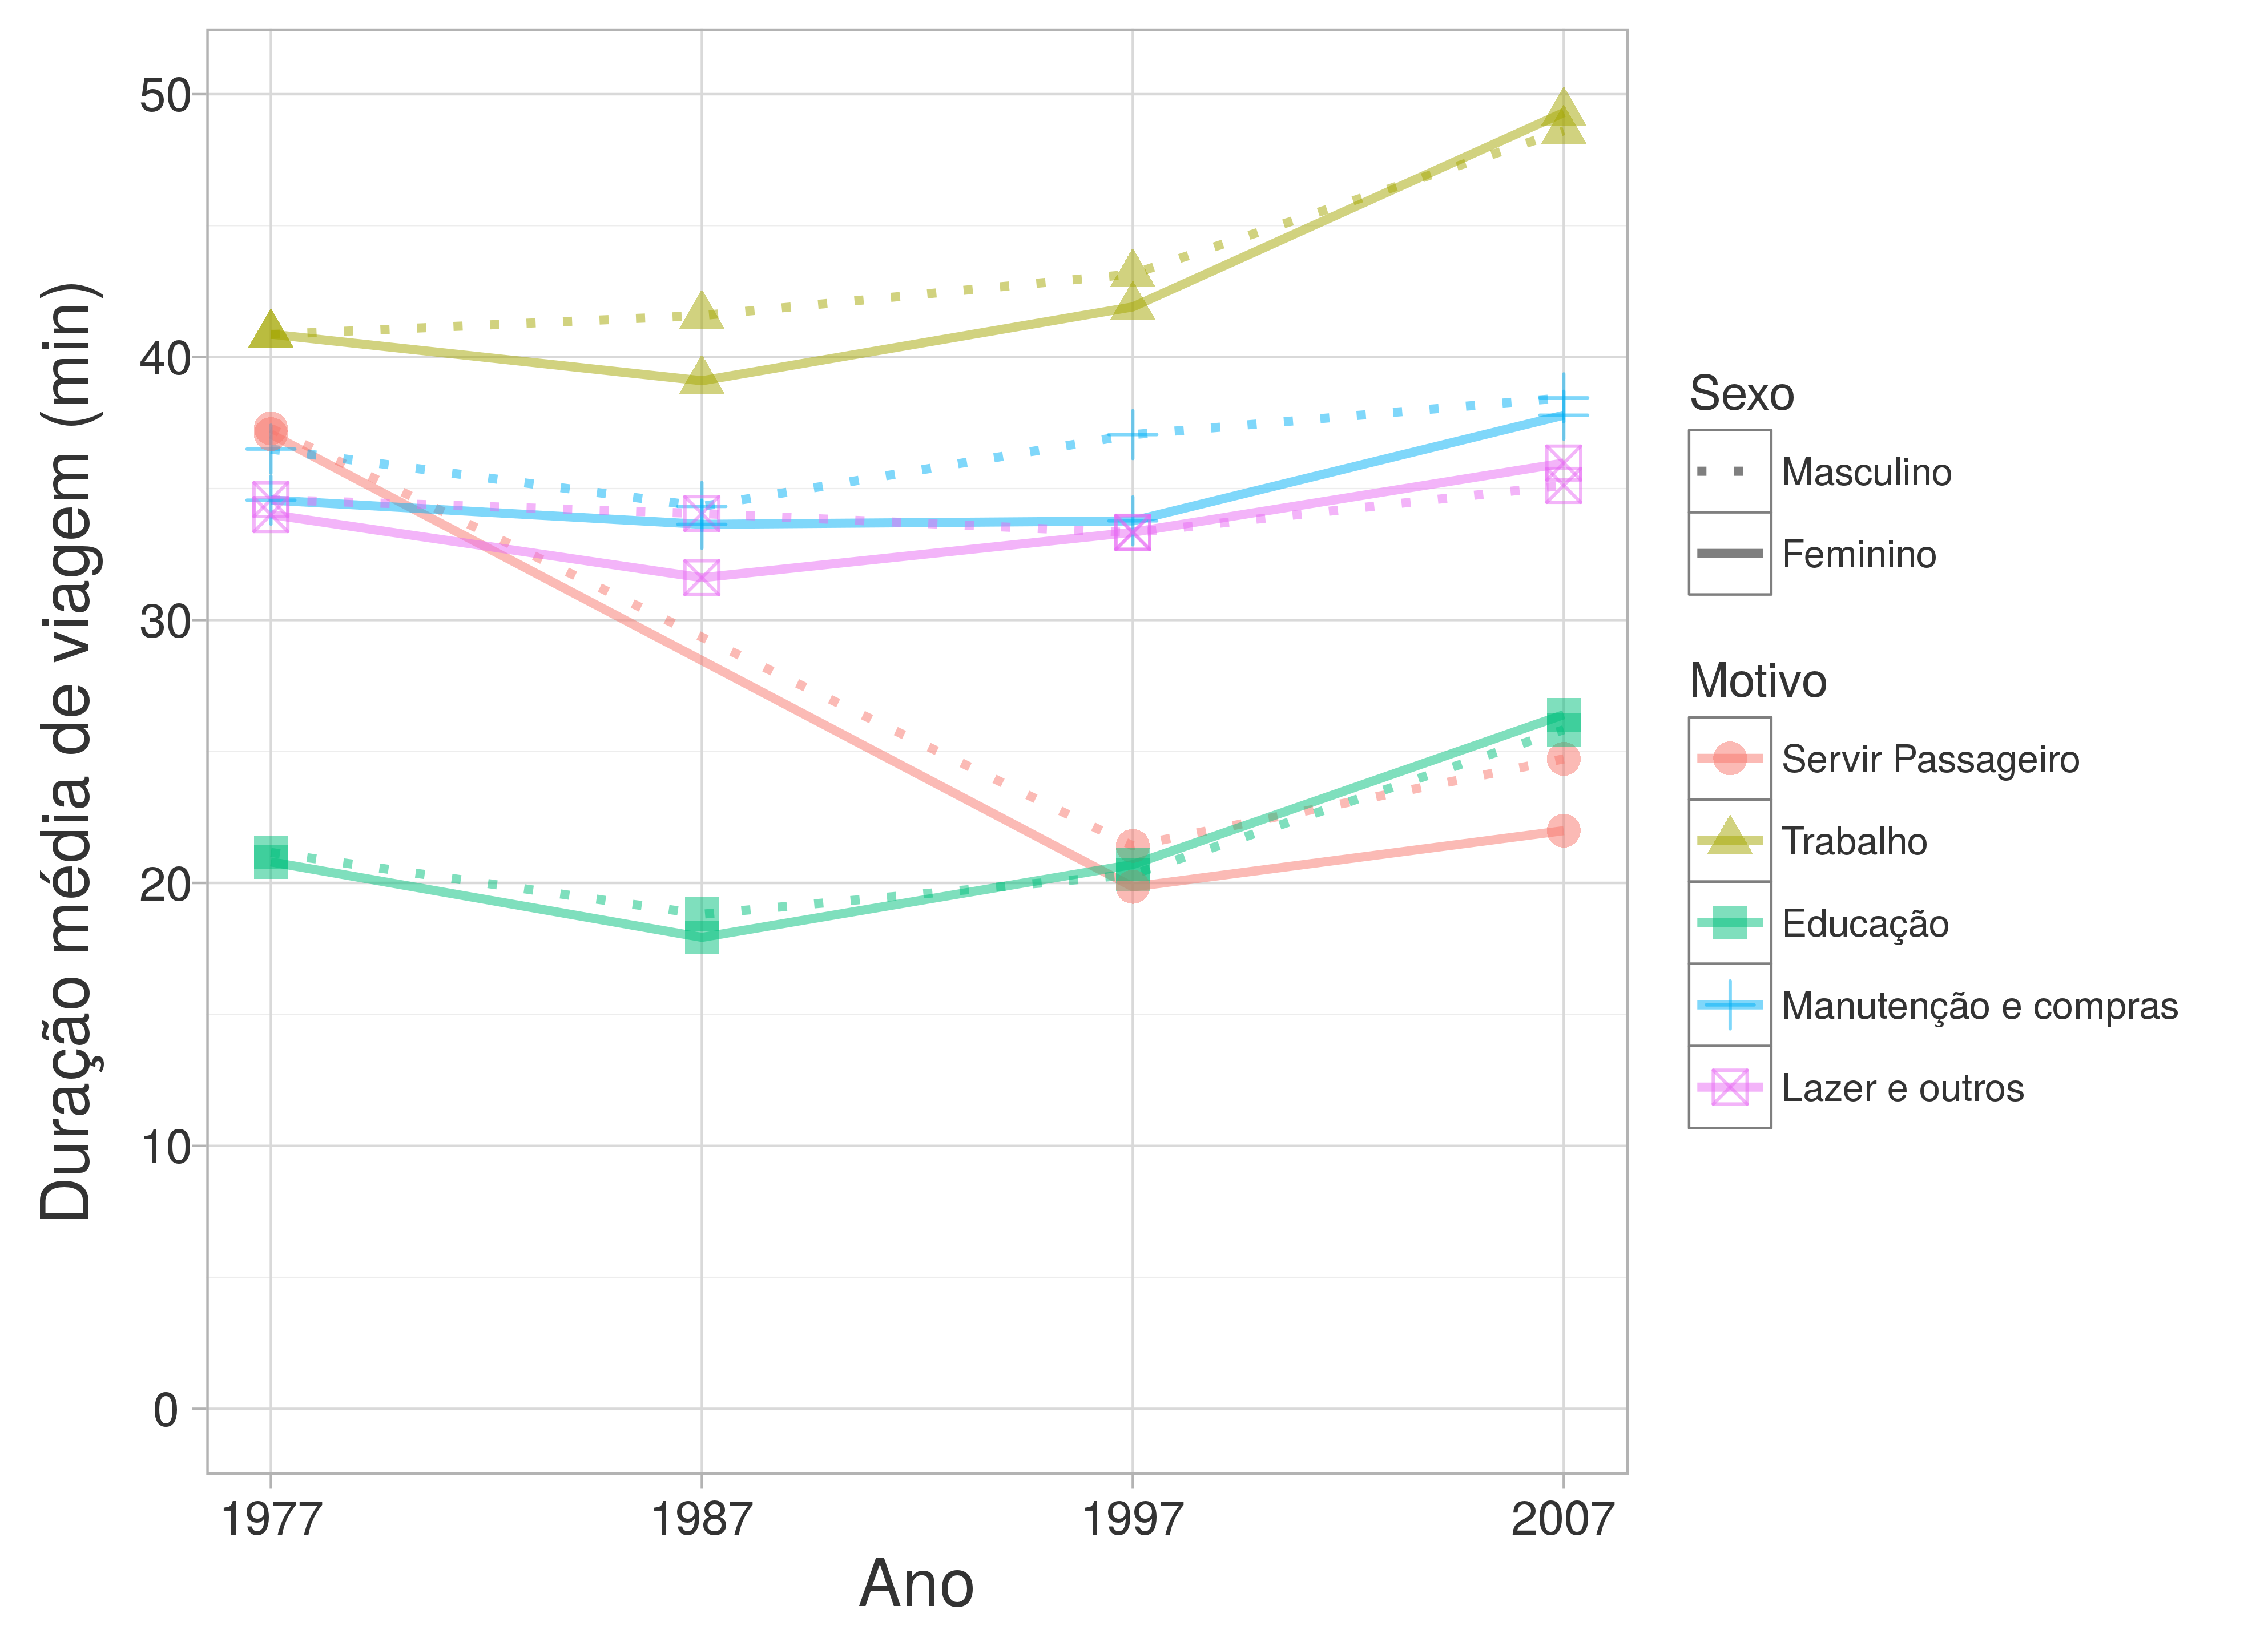
\includegraphics[width=1\textwidth]{./imagens/duracao-motivo.png}%
    \end{center}%
%    \fonte{Compilação própria}
\end{grafico}%
% Estatísticas para registros com F_VIAG==1 e SEXO
% Expandido com FE_VIAG

%TODO ?? Fazer DURACAO (médias) por faixas etárias / situação familliar
%Tendo em vista ainda as questões apontadas na revisão de literatura a respeito da mobilidade/imobilidade das pessoas e formas de mensurá-la, pretende-se avaliar a distância média das viagens em função das variáveis sexo, idade, renda familiar, renda individual, estado civil e presença de filhos da família \cite{ROSENBLOOM2006,SHEARMUR2006,HANSON2010}.

Em “Estatísticas sob Suspeita”, \citeauthoronline{CARRASCO2012} (\citeyear{CARRASCO2012}, p.100-101) propõe indicadores com base na experiência das mulheres e, especificamente, no capítulo relativo ao acesso à mobilidade e ao planejamento territorial, recomenda a formulação e consideração dos seguintes indicadores quando da formulação de políticas públicas:
motivos dos deslocamentos, meio utilizado nos deslocamentos e distâncias dos deslocamentos, entre outros.
Anteriormente foram apresentados os panoramas de motivos e modos, agora, serão exploradas as distâncias de deslocamento.

A variável de distância da viagem (\textbf{DIST_VIAG}) contém a distância euclidiana entre as coordenadas x e y de origem e as coordenadas x e y de destino, com as limitações que a determinação dessas coordenadas impõem, já que foram calculadas a partir dos centroides das subzonas ou zonas (na ausência das subzonas). 

%TODO -> Fazer estatísticas de PESS_DIST_TOT
%Dalmaso e Strambi (2006) estudaram como o comportamento da distância total viajada por uma pessoa relaciona-se com seus atributos individuais sexo e idade.


\clearpage
\section{Análise de conglomerados para identificação de grupos}\label{sec:analises-clusters}

A análise de conglomerados tem como objetivo segregar elementos (observações) “em grupos homogêneos internamente, heterogêneos entre si e mutuamente exclusivos, a partir de determinados parâmetros conforme uma medida similaridade ou distância” \cite[p.196]{FAVERO2009}.  Esta técnica estatística de interdependência foi escolhida pois se deseja agrupar as pessoas, ou mesmo famílias, em grupos homogêneos em função da similaridade do comportamento de viagens.

%Vários trabalhos têm usados análises de agrupamento no estudo de XXXXX %TODO

Foi utilizada a função \textit{hclust} do pacote \textit{stats}
\footnote{Também existe a função \textit{agnes}, do pacote \textit{cluster}, cuja documentação está disponível em \url{https://cran.r-project.org/web/packages/cluster/cluster.pdf} e que se propõe a resolver o mesmo algoritmo. Porém, o resultado obtido dos três pacotes (stats, fastcluster e cluster) não foram iguais. \citeauthoronline{MURTAGH1975} (\citeyear{MURTAGH1975}) já apontavam divergência entre as funções \textit{hclust} e \textit{agnes} quando aplicadas à mesma matriz de distâncias.} \cite{RTEAM2011} para realizar as análises hierárquicas de conglomerados. Devido ao tamanho da base de dados e ao baixo desempenho em termos computacionais do pacote \textit{stats}, preferiu-se a função \textit{hclust} do pacote \textit{fastcluster}
\footnote{Detalhes da implementação disponível em \citeauthoronline{MULLNER2011} (\citeyear{MULLNER2011}).}. 
Segundo \citeauthoronline{MULLNER2013} (\citeyear{MULLNER2013}), no pior caso, a função do pacote \textit{stats} tem seu tempo de execução proporcional a $N^3$, já a mesma função no pacote \textit{fastcluster}, é poporcional a $N^2$. As análises de conglomerados não hierárquicas foram executadas pela função kmeans do pacote \textit{stats}. Na Figura \ref{fig:roteiro-cluster} pode-se observar os passos realizados nesta etapa de análise.

\begin{figure}[htb]%
    \caption{\label{fig:roteiro-cluster}Etapas para a realização de análise de conglomerados (\textit{clusters})}%
    \begin{center}%
        \includegraphics[width=0.30\textwidth]{./imagens/roteiro-cluster.eps}%
    \end{center}%
%    \fonte{Elaboração própria}
\end{figure}%


Na \textbf{etapa A}, foram delimitados dois conjuntos iniciais de variáveis de análise:
\begin{compactitem}
\item \textbf{conjunto I}: De atributos de viagem, relativas à família, a saber: FAM_DIST_TOT, FAM_DIST_MED, FAM_DURACAO_TOT, FAM_DURACAO_MED, FAM_VIAG_TOT;
\item \textbf{conjunto II}: De atributos de viagem, relativas à pessoa, a saber: PESS_DIST_TOT, PESS_DIST_MED, PESS_DURACAO_TOT, PESS_DURACAO_MED, PESS_MODO_ONIBUS, PESS_MODO_DIRIG, PESS_MODO_PASS, PESS_MODO_TREM, PESS_MODO_MOTO, PESS_MODO_BICI, PESS_MODO_APE, PESS_MODO_OUTROS, PESS_NO_MODOS, PESS_MOTIVO_TRAB, PESS_MOTIVO_EDUC, PESS_MOTIVO_RES, PESS_MOTIVO_SERV_PAS, PESS_MOTIVO_MANUT_COMPRAS, PESS_MOTIVO_LAZER_OUTROS, PESS_NO_MOTIVOS, PESS_PER_MADRUG, PESS_PER_COM_MAN, PESS_PER_MANHA, PESS_PER_MEIODIA, PESS_PER_TARDE, PESS_PER_COM_NOI, PESS_PER_NOITE, PESS_NO_PERIODOS, TOT_VIAG.
\end{compactitem}

Ocorre em diversos bancos de dados, inclusive neste, de se desejar analisar variáveis cujas unidades e ordens de grandezas não são as mesmas.
\citeauthoronline{FARIA2009} (\citeyear{FARIA2009}) indica que há duas razões para padronizar dados: (i) "evitar que as unidades escolhidas para mensurar as características afetem arbitrariamente a similaridade entre indivíduos", e (ii) fazer com "que as características contribuam igualmente na avaliação da similaridade entre indivíduos". Se houver alguma unidade de medição que tenha uma amplitude maior que as demais (como é o caso das distâncias totais da família em relação à distância média da pessoa), ela terá maior peso na análise de \textit{cluster}. Então, para mitigar o efeito dessas diferenças é indicado padronizar os dados antes de submetê-los à análise de conglomerados. Ao fazer isso, o pesquisador assume que a importância da variável decresce conforme a variabilidade aumenta \cite{EVERITT2011}. Há diversas formas de fazer essa padronização, as mais comuns são \textit{z-scores} e normalização \cite{FAVERO2009}. Há também possibilidades como dividir pela mediana dos desvios absolutos ou pelos intervalos de valores da variável \apud{GNANA1995}{EVERITT2011}, porém, a complexidade deste últimos métodos não se justificam frente ao conjunto de dados em discussão. Assim, na \textbf{etapa B} do presente trabalho, foi feita padronização das variáveis pelo método \textit{z-scores} conforme Equações \eqref{eq:z-score}, \eqref{eq:media} e \eqref{eq:desvio-padrao}.

\begin{equation}\label{eq:z-score}
Z(x)_{i} = \frac{x_{i} - \bar{x}}{\sigma(x)}
\end{equation}
sendo:
\begin{equation}\label{eq:media}
\bar{x} = \frac{1}{n} \sum_{i=1}^{n} x_{i}
\end{equation}

\begin{equation}\label{eq:desvio-padrao}
\sigma(x) = \sqrt{\frac{1}{(n-1)} \sum_{i=1}^{n}(x_{i}-\bar{x})^2 }
\end{equation}

\newpage
Um dos principais problemas das técnicas de aglomeração não hierárquica (K-means) é definir de início o número de \textit{clusters} desejado \cite{HARTIGAN1985, FAVERO2009, EVERITT2011}. Existem algumas técnicas para essa determinação:

\begin{compactitem}[]
\item (i) A \textbf{\textit{upper tail rule}} que considera os valores de fusão como uma série. Calcula-se a média, desvio padrão, estatística t como o desvio normalizado a partir da média. Em seguida, calcula-se o desvio padrão para cada valor de fusão (assumida distribuição normal), seleciona o primeiro ``significativo'' como sendo aquele cuja estatística t exceda o nível de 5\% de significância. Assim, a hipótese nula é que o valor fusão do k-ésimo termo advém da distribuição normal dos valores de fusão \cite{MOJENA1977}.
\item (ii) O \textbf{índice RMSSTD} (\textit{root mean square standard deviation}), ou raiz quadrada do desvio padrão médio (ver Equação \eqref{eq:RMSSTD}, calcula a homogeneidade dos agrupamentos \cite{SHARMA1996}, de maneira que quanto mais compactos os grupos, menor o valor desta estatística.
 
\begin{equation}\label{eq:RMSSTD} 
RMSSTD = \sqrt{\frac{\displaystyle\sum_{\substack{i=1\\
j=1}}^{\substack{nc\\
d}}\displaystyle\sum_{k=1}^{n_{j}}(x_{k}-\bar{x}_{j})^2}{\displaystyle\sum_{\substack{i=1\\
j=1}}^{\substack{nc\\
d}}(n_{ij}-1)}}
\end{equation}

\item (iii) O \textbf{índice $R^2$ ajustado} (ver Equação \eqref{eq:RS}), indica dissimilaridade entre agrupamentos \cite{SHARMA1996}, assim, quanto mais alto o valor de $R^2$ ajustado, mais dissimilaridade existe entre os grupos. O pesquisador pode estabelecer um valor desejado para $R^2$ e, a partir daí, determinar o número de \textit{clusters}.

\begin{equation}\label{eq:RS} 
R^2 = \frac{\left[\displaystyle\sum_{\substack{i=1\\
j=1}}^{\substack{nc\\
d}}\sum_{k=1}^{n_{j}}(x_{i}-\bar{x}_{j})^2\right]-\left[\displaystyle\sum_{\substack{i=1\\
j=1}}^{\substack{nc\\
d}}\displaystyle\sum_{k=1}^{n_{ij}}(x_{k}-\bar{x}_{j})^2\right]}{\displaystyle\sum_{j=1}^{d}\displaystyle\sum_{k=1}^{n_{j}}(x_{k} - \bar{x}_{j})^2 }
\end{equation}

\item (iv) O \textbf{\textit{best cut}} é um método que se baseia em um dendrograma (representação bidimensional em forma de árvore) que deve ser cortado quando as diferenças entre grupos forem visualmente mais significativas. Nesta representação, as linhas são ligadas segundo níveis de similaridade que agregará os indivíduos \cite{EVERITT2011}.
\end{compactitem}

Então, primeiro foi realizada a aglomeração hierárquica para definir as quantidades grupos.
No método hierárquico, se há n observações (linhas), parte-se de n grupos, ou seja, existe uma observações por grupo. A partir de medidas de similaridade, num processo iterativo, as observações vão sendo agrupadas até que se chegue a um único grupo no final. Segundo \cite{MAXWELL1977}, primeiro é feita a conversão da matriz \textit{n versus p} de dados em uma matriz \textit{n versus n} de medidas de similaridade ou dissimilaridade, tendo-se \textit{n} unidades amostrais e \textit{p} características.
Optou-se por primeiro utilizar o \textbf{\textit{best cut}} com os dendrogramas
\footnote{Os dendrogramas gerados admitiram escala não-monotônica.} 
e, em seguida, seriam avaliados os índices \textbf{RMSSTD} e \textbf{$R^2$ ajustado} de 90\%.

As medidas de (dis)similaridade podem ser de distância, correlação ou associação, esta última indicada para variáveis qualitativas. Como as variáveis selecionadas na \textbf{etapa A} são métricas ou \textit{dummies}, são indicadas medidas de distância ou correlação. 
Na Tabela \ref{tab:dist-cluster} é possível observar algumas das principais medidas de dissimilaridade comumente utilizadas.
Optou-se, na \textbf{etapa C}, pela medida de distância euclidiana, indicada pela literatura \apud{HAIR2005}{FAVERO2009}, 
a ser adotada em conjunto com os métodos de agrupamento Ward \cite{WARD1963} e centroide. O arcabouço teórico indica que tanto as distâncias euclidianas quanto as euclidianas quadráticas resultarão nos mesmos \textit{clusters} e, no caso da função \textit{hclust} utilizada, a distância padrão calculada é a euclidiana.



\begin{table}[htb]
    \IBGEtab{
	    \renewcommand{\arraystretch}{2.8}
        \caption{Medidas de dissimilaridade utilizadas em análise de \textit{cluster}}
		\label{tab:dist-cluster}
    }{%
	    \begin{tabular}{ll}
        \toprule
		    \headerTabCenterCell{Medida} &
	   	    \headerTabCenterCell{Fórmula}\\
		    \midrule \midrule
						Distância Euclidiana &
						\begin{math}
						    d_{ij}=\left[\displaystyle\sum_{k=1}^{p}w_{k}^2(x_{ik}-x_{jk})^2\right]^{}1/_2
						\end{math} \\
		    %\midrule
						Distância \textit{city block} &
						\begin{math}
                d_{ij}=\displaystyle\sum_{k=1}^{p}w_{k}|x_{ik}-x_{jk}|
						\end{math} \\
				%\midrule
				    Distância de Minkowski &
				    \begin{math}
				        d_{ij}=\left(\displaystyle\sum_{k=1}^{p}w_{k}^{r}|x_{ik}-x_{jk}|^{r}\right)^{{}1/_r} \quad (r\geq1)
				    \end{math} \\
				%\midrule
				    Distância de Canberra &
				    \begin{math}
				        d_{ij}= \begin{cases}
				                  0 & \quad \text{for } x_{ik}=x_{jk}=0 \\
				                  \displaystyle\sum_{k=1}^{p}w_{k}|x_{ik}-x_{jk}|/(|x_{ik}|+|x_{jk}|) & \quad \text{for } x_{ik} \neq 0 \text{ or } x_{jk} \neq 0\\
				                \end{cases}
				    \end{math} \\
			\bottomrule	
		\end{tabular}
    }{%
		\fonte{\cite{EVERITT2011}}
		}
\end{table}

Na \textbf{etapa D}, foi feita a aglomeração para o \textbf{conjunto I} de variáveis da família e para o \textbf{conjunto II} de variáveis da pessoa, utilizando tanto o método Ward quanto o centroide, utilizando filtros que captassem a ocorrência da família (F_FAM=1) ou da pessoa (F_PESS=1), respectivamente, para que não houvesse repetição indevida de famílias ou pessoas. Essas aglomerações foram feitas sem distinção dos anos e resultaram nos dendrogramas apresentados nas Figuras \ref{fig:cluster-fam-total} e \ref{fig:cluster-pess-total}. Percebe-se que a forma do dendrograma difere muito pouco entre os métodos Ward e centroide para o mesmo conjunto de variáveis.
%Para as análises seguintes foi escolhido o centroide pois segundo \apudonline{HAIR2005}{FAVERO2009}  “este método é mais robusto para observações atípicas”. 

Considerando o \textbf{best cut} observa-se que os dendrogramas que partiram das variáveis de família, indicam 4 como sendo um número de \textit{clusters} interessante de ser dado como \textit{input} do método K-means - observar seções S da Figura \ref{fig:cluster-fam-total}. Os índices \textbf{RMSSTD} e \textbf{$R^2$} ajustado, conforme pode ser visto no Gráfico \ref{graf:rmsstd-r2-cluster-fam-total}, também corroboram para a divisão em 4 grupos, representando 90\% da variância.

Partindo do conjunto de atributos de viagens relativas às pessoas, o \textbf{best cut} dos dendrogramas resultantes também indicam 4 \textit{clusters}, seja pelo método Ward, seja pelo centroide - observar seções S da Figura \ref{fig:cluster-pess-total}. Os índices \textbf{RMSSTD} e \textbf{$R^2$} ajustado, conforme pode ser visto no Gráfico \ref{graf:rmsstd-r2-cluster-pess-total}, também corroboram para a divisão em 4 grupos, representando mais de 90\% da variância.

Assim, na \textbf{etapa E}, definiu-se que seriam adotados 4 \textit{clusters}, tanto para o conjunto de variáveis I (de família) como o II (de pessoas) no método de aglomeração K-means
\footnote{ A função \textit{kmeans} do pacote \textit{stats} do software R implementa o algoritmo de \citeauthoronline{HARTIGAN1979} (\citeyear{HARTIGAN1979}) por padrão para sua execução, que utiliza também a distância euclidiana como medida de similaridade.} 
que, segundo \apudonline{GOUVEA2006}{FAVERO2009}, minimiza a variância interna aos grupos e maximiza a variância entre grupos.

\begin{figure}[htb]%
    \caption{\label{fig:cluster-fam-total}Dendrograma resultante da análise de conglomerados hierárquico, para o conjunto de atributos de viagens relativas às famílias}%
    \begin{center}%
        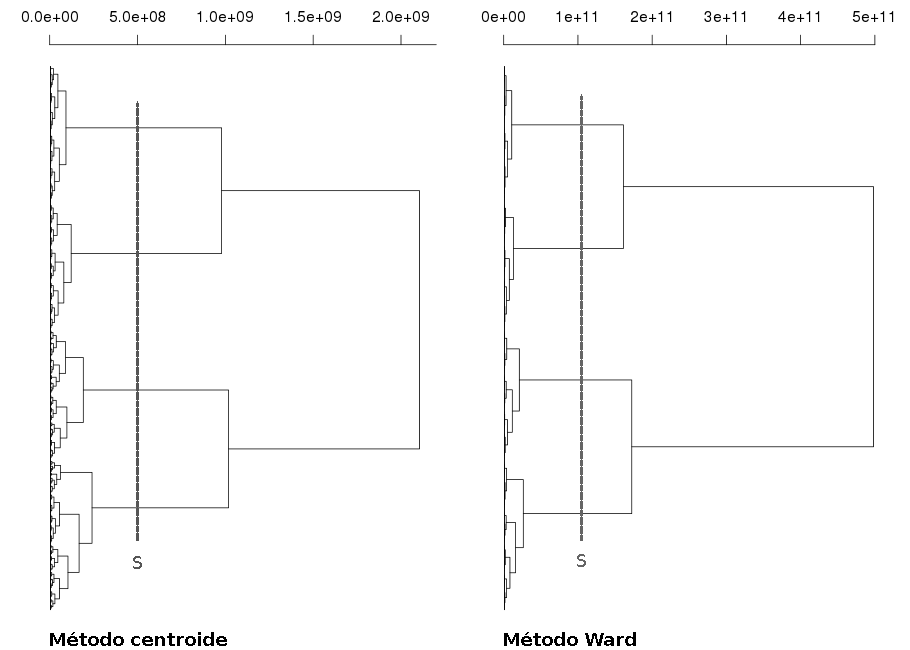
\includegraphics[width=0.95\textwidth]{./imagens/dendro-hierarq-cluster-familia-total-final.png}%
    \end{center}%
%    \fonte{Elaboração própria}
\end{figure}%


\begin{grafico}[htb]%
    \caption{\label{graf:rmsstd-r2-cluster-fam-total}Avaliação do número de \textit{clusters} para o conjunto de atributos de viagens relativas às famílias}%
    \begin{center}%
        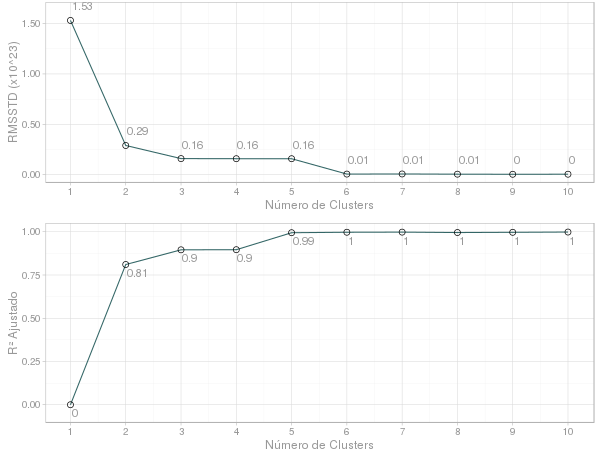
\includegraphics[width=0.8\textwidth]{./imagens/No-clusters-R2-RMSSTD-familia.png}%
    \end{center}%
%    \fonte{Elaboração própria}
\end{grafico}%


\begin{figure}[htb]%
    \caption{\label{fig:cluster-pess-total}Dendrograma resultante da análise de conglomerados hierárquico, para o conjunto de atributos de viagens relativas às pessoas}%
    \begin{center}%
        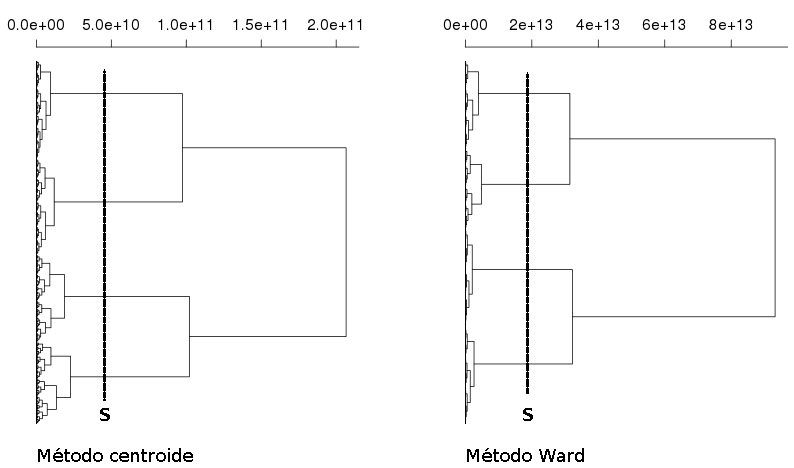
\includegraphics[width=0.95\textwidth]{./imagens/dendro-hierarq-cluster-pessoa-total-final.png}%
    \end{center}%
%    \fonte{Elaboração própria}
\end{figure}%

\clearpage

\begin{grafico}[htb]%
    \caption{\label{graf:rmsstd-r2-cluster-pess-total}Avaliação do número de \textit{clusters} para o conjunto de atributos de viagens relativas às pessoas}%
    \begin{center}%
        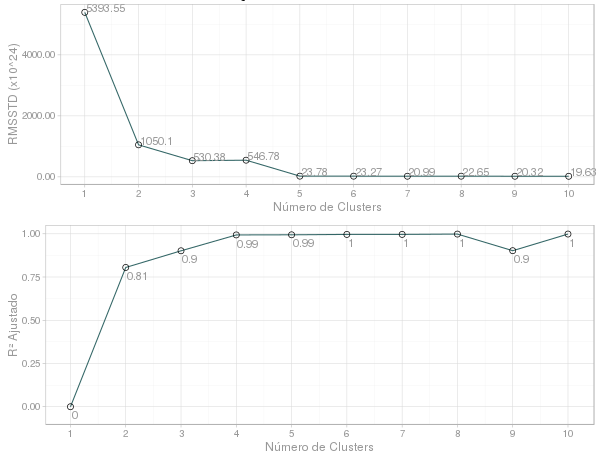
\includegraphics[width=0.8\textwidth]{./imagens/No-clusters-R2-RMSSTD-pessoas.png}%
    \end{center}%
%    \fonte{Elaboração própria}
\end{grafico}%

Na \textbf{etapa F}, foram formados então quatro agrupamentos para atributos de viagens de \textbf{família}, pelo método Ward. Observa-se que os grupos formados correspondem exatamente às observações de cada ano. 
Ou seja, o \textit{cluster} 1 agregou as observações de 1977, o \textit{cluster} 2 agregou as observações de 1987, e assim por diante - ver Tabela \ref{tab:cluster-fam-ward-4}. Entretanto, utilizando o método centroide, houve a união de 1997 e 2007, além da separação de 1987 em dois grupos distintos - ver Tabela \ref{tab:cluster-fam-centroide-4}.
Ao analisar os quatro agrupamentos para atributos de viagens de \textbf{pessoas}, tanto com o método centroide quanto com o Ward, os grupos formados também correspondem exatamente às observações de cada ano. 

\begin{table}[htb]
    \IBGEtab{%\renewcommand{\arraystretch}{1.5}%%\ABNTEXfontereduzida%
%	    \renewcommand{\arraystretch}{1.5}
        \caption{Resultado do agrupamento de 4 \textit{clusters}, por atributos de viagens de família - método Ward}
		\label{tab:cluster-fam-ward-4}
    }{%
	    \begin{tabular}{P{1.00cm} P{3.00cm} P{3.00cm} P{3.00cm} P{3.00cm}}
            \toprule
	           \headerCenterCell{\textit{Cluster} nº} &
   	           \headerCenterCell{\% de famílias de 1977} &
   	           \headerCenterCell{\% de famílias de 1987} &   	           
   	           \headerCenterCell{\% de famílias de 1997} &   	           
   	           \headerCenterCell{\% de famílias de 2007}\\
		    \midrule \midrule
				1& % É  o 2, na verdade
		    	100&
		    	0&
		    	0&
				0\\
			\midrule
				2& % É o 1, na verdade
				0&
				100&
				0&
		        0\\
			\midrule
				3& % É o 3 mesmo
				0&
				0&
				100&
		        0\\
			\midrule
				4& % È o 4 mesmo
				0&
				0&
				0&
		        100\\
			\bottomrule	
		\end{tabular}
    }{%
		%\fonte{Elaboração própria}
	}
\end{table}

\begin{table}[htb]
    \IBGEtab{%\renewcommand{\arraystretch}{1.5}%%\ABNTEXfontereduzida%
%	    \renewcommand{\arraystretch}{1.5}
        \caption{Resultado do agrupamento de 4 \textit{clusters}, por atributos de viagens de família - método centroide}
		\label{tab:cluster-fam-centroide-4}
    }{%
	    \begin{tabular}{P{1.00cm} P{3.00cm} P{3.00cm} P{3.00cm} P{3.00cm}}
            \toprule
	           \headerCenterCell{\textit{Cluster} nº} &
   	           \headerCenterCell{\% de famílias de 1977} &
   	           \headerCenterCell{\% de famílias de 1987} &   	           
   	           \headerCenterCell{\% de famílias de 1997} &   	           
   	           \headerCenterCell{\% de famílias de 2007}\\
		    \midrule \midrule
				1& % É  o 3, na verdade
		    	100&
		    	0&
		    	0&
				0\\
			\midrule
				2& % É o 1, na verdade
				0&
				100&
				0&
		        0\\
			\midrule
				3& % É o 2, na verdade
				0&
				100&
				0&
		        0\\
			\midrule
				4& % È o 4 mesmo
				0&
				0&
				51,94&
		        48,06\\
			\bottomrule	
		\end{tabular}
    }{%
		%\fonte{Elaboração própria}
	}
\end{table}

\newpage
Tomando três agrupamentos, tendo em foco a \textbf{família}, pelo método Ward os grupos que se unem são os anos de 1997 e 2007. Já pelo método centroide, 1997 destaca-se de 2007, enquanto 1987 se agrega completamente a 1977, conforme pode ser observado nas Tabelas \ref{tab:cluster-fam-ward-3} e \ref{tab:cluster-fam-centroide-3}. Ao focar os atributos de viagens das \textbf{pessoas}, agrupadas em três \textit{clusters}, não houve diferença no resultado utilizando Ward ou centroide, tal como foi com quatro grupos. 

\begin{table}[htb]
    \IBGEtab{%\renewcommand{\arraystretch}{1.5}%%\ABNTEXfontereduzida%
%	    \renewcommand{\arraystretch}{1.5}
        \caption{Resultado do agrupamento de 3 \textit{clusters}, por atributos de viagens de família - método Ward}
		\label{tab:cluster-fam-ward-3}
    }{%
	    \begin{tabular}{P{1.00cm} P{3.00cm} P{3.00cm} P{3.00cm} P{3.00cm}}
            \toprule
	           \headerCenterCell{\textit{Cluster} nº} &
   	           \headerCenterCell{\% de famílias de 1977} &
   	           \headerCenterCell{\% de famílias de 1987} &   	           
   	           \headerCenterCell{\% de famílias de 1997} &   	           
   	           \headerCenterCell{\% de famílias de 2007}\\
		    \midrule \midrule
				1& 
		    	100&
		    	0&
		    	0&
				0\\
			\midrule
				2& 
				0&
				100&
				0&
		        0\\
			\midrule
				3& % É o 3 mesmo
				0&
				0&
				46,5&
		        53,5\\
			\bottomrule	
		\end{tabular}
    }{%
		%\fonte{Elaboração própria}
	}
\end{table}

\begin{table}[htb]
    \IBGEtab{%\renewcommand{\arraystretch}{1.5}%%\ABNTEXfontereduzida%
%	    \renewcommand{\arraystretch}{1.5}
        \caption{Resultado do agrupamento de 3 \textit{clusters}, por atributos de viagens de família - método centroide}
		\label{tab:cluster-fam-centroide-3}
    }{%
	    \begin{tabular}{P{1.00cm} P{3.00cm} P{3.00cm} P{3.00cm} P{3.00cm}}
            \toprule
	           \headerCenterCell{\textit{Cluster} nº} &
   	           \headerCenterCell{\% de famílias de 1977} &
   	           \headerCenterCell{\% de famílias de 1987} &   	           
   	           \headerCenterCell{\% de famílias de 1997} &   	           
   	           \headerCenterCell{\% de famílias de 2007}\\
		    \midrule \midrule
				1&
		    	48,1&
		    	51,9&
		    	0&
				0\\
			\midrule
				2&
				0&
				0&
				100&
		        0\\
			\midrule
				3&
				0&
				0&
				0&
		        100\\
			\bottomrule	
		\end{tabular}
    }{%
		%\fonte{Elaboração própria}
	}
\end{table}


\newpage
Na Tabela \ref{tab:cluster-pess-ward-centroide-3} é possível observar que 1977 e 1987 se separam, e 1997 se une a 2007. 
Percebe-se que a variável ANO, embora não inserida nas análises de conglomerados, acabou sendo a grande diferenciadora dos grupos.
Esses resultados levantam a questões como:
\begin{compactitem}[]
\item (i) o tempo (em si ou como \textit{proxy} de outras variáveis) é uma categoria de análise relevante;
\item (ii) pode ter havido evolução no método de pesquisa e o agrupamento temporal esteja captando este efeito; 
\item (iii) parece haver semelhanças entre 2007 e 1997;
\item (iv) parece haver semelhanças entre 1987 e 1977, talvez mais fracas que as entre 2007 e 1997;
\item (v) não parece haver semelhanças tão fortes entre 1987 e 1997.
\end{compactitem}
    
\begin{table}[htb]
    \IBGEtab{%\renewcommand{\arraystretch}{1.5}%%\ABNTEXfontereduzida%
	    \renewcommand{\arraystretch}{1.5}
        \caption{Resultado do agrupamento de 3 \textit{clusters}, por atributos de viagens de pessoas - métodos Ward e centroide}
		\label{tab:cluster-pess-ward-centroide-3}
    }{%
	    \begin{tabular}{P{1.00cm} P{3.00cm} P{3.00cm} P{3.00cm} P{3.00cm}}
            \toprule
	           \headerCenterCell{\textit{Cluster} nº} &
   	           \headerCenterCell{\% de pessoas de 1977} &
   	           \headerCenterCell{\% de pessoas de 1987} &   	           
   	           \headerCenterCell{\% de pessoas de 1997} &   	           
   	           \headerCenterCell{\% de pessoas de 2007}\\
		    \midrule \midrule
				1& 
		    	100&
		    	0&
		    	0&
				0\\
			\midrule
				2& 
				0&
				100&
				0&
		        0\\
			\midrule
				3&
				0&
				0&
				51,9&
		        48,1\\
			\bottomrule	
		\end{tabular}
    }{%
		%\fonte{Elaboração própria}
	}
\end{table}

Sob a perspectiva de gênero, retomando os dados de participação na PEA apresentados no Gráfico \ref{graf:evolucao-pea}, 
percebe-se o $\Delta_{1991-1980} = 6,3\%$, $\Delta_{2000-1991} = 11,2\%$ e $\Delta_{2010-2000} = 4,8\%$. Embora, os dados da PEA refiram-se aos anos 1980, 1991, 2000 e 2010, não coincidentes com os das Pesquisas OD (1977, 1987, 1997 e 2007), se tomarmos os anos mais próximos como referencial de análise, percebemos que o maior salto na participação feminina no mercado de trabalho ocorreu entre 2000 e 1991, e que as pesquisas que parecem apresentar a maior dissemelhança são as OD-1997 e OD-1987. Não é possível fazer muitas afirmações a partir somente deste paralelo, entretanto, isto pode ser um indicativo de que os padrões de mobilidade se alteraram sob efeito do tempo e também considerando o gênero como categoria de análise.
 
Para explorar melhor o que ocorre dentro de cada grupo e o que ocorre entre grupos foram analisadas as características de viagens, das pessoas e das famílias a partir da segregação dos 4 \textit{clusters} resultantes - ver Anexo \ref{chap:anexo_4_clusters_td}.

No agrupamento feito por atributos de viagens da família pelo método Ward, observa-se que a maior diferença percentual entre valores mínimo e máximo entre grupos ocorreu com a variável ``\% de pessoas com superior completo'' (76\%) e a menor diferença ocorreu com a variável ``sexo'' (4\%).
A Tabela \ref{tab:cluster-fam-ward-top10} apresenta as variáveis que apresentaram as diferenças percentuais entre valores máximos e mínimos superiores a 50\%.
Para estas nove variáveis foi realizado teste qui-quadrado de Pearson (de independência) em relação à variável que indica os \textit{clusters} e todas mostraram-se significativas considerando um intervalo de confiança de 99\%. 

\begin{table}[htb]
    \IBGEtab{%\renewcommand{\arraystretch}{1.5}%%\ABNTEXfontereduzida%
	    \renewcommand{\arraystretch}{1.5}
        \caption{Ordenamento das variáveis pelas maiores diferenças percentuais - para agrupamento FAM_CLUSTER_WARD4}
		\label{tab:cluster-fam-ward-top10}
    }\\
		    \midrule \midrule
		    	1º&
				\% de pessoas com superior completo& 
				76\\
			\midrule
				2º& 
				\% de pessoas com situação famíliar `outros'&
		        71\\
			\midrule
				3º& 
				\% de famílias na Classe A&
		        67\\		        
			\midrule
				4º& 
				\% de pessoas com médio completo ou superior incompleto&
		        66\\	
			\midrule
				5º& 
				\% de pessoas que servem passageiro no destino&
		        65\\			        
			\midrule
				6º& 
				\% de famílias na Classe E&
		        61\\
			\midrule
				7º& 
				\% de famílias com presença de criança entre 0 e 4 anos&
		        60\\
			\midrule
				8º& 
				\% de pessoas empregadas&
		        59\\
			\midrule
				9º&
				\% de famílias com presença de criança entre 5 e 9 &
		        56\\
			\bottomrule	
		\end{tabular}
    }{%
		%\fonte{Elaboração própria}
	}
\end{table}

No agrupamento feito por atributos de viagens da família pelo método centroide, observa-se que a maior diferença percentual entre valores mínimo e máximo entre grupos ocorreu com a variável ``\% de famílias na Classe A'' (79\%) e a menor diferença ocorreu com a variável ``Média da quantidade de trabalhadores (as) na família'' (2\%).
Vale mencionar que as diferenças percentuais entre valores mínimo e máximo ocorreram entre os grupos 2 (uma parte de 1987) e 3 (outra parte de 1987) em relação as seguintes características: (i) distância média por viagem da pessoa; (ii) distância média por pessoa da família; (iii) \% de pessoas do sexo feminino e (iv) \% de outros parentes / agregados.

A Tabela \ref{tab:cluster-fam-centr-top10} apresenta as variáveis que apresentaram as diferenças percentuais entre valores máximos e mínimos superiores a 50\%.
Para estas nove variáveis foi realizado teste qui-quadrado de Pearson (de independência) em relação à variável que indica os \textit{clusters} e todas mostraram-se significativas considerando um intervalo de confiança de 99\%. 

\begin{table}[htb]
    \IBGEtab{%\renewcommand{\arraystretch}{1.5}%%\ABNTEXfontereduzida%
	    \renewcommand{\arraystretch}{1.5}
        \caption{Ordenamento das variáveis pelas maiores diferenças percentuais - para agrupamento FAM_CLUSTER_CENTROIDE4}
		\label{tab:cluster-fam-centr-top10}
    }\\
		    \midrule \midrule
				1º& 
				\% de famílias na Classe A&
		        79\\		        
			\midrule
				2º& 
				\% de pessoas empregadas&
		        76\\
			\midrule			
		    	3º&
				\% de pessoas com superior completo& 
				73\\
			\midrule
				4º& 
				\% de pessoas com situação famíliar `outros'&
		        71\\
			\midrule
				5º& 
				\% de famílias na Classe E&
		        66\\
			\midrule
				6º& 
				\% de pessoas com médio completo ou superior incompleto&
		        65\\	
			\midrule
				7º& 
				\% de pessoas que servem passageiro no destino&
		        61\\			        
			\midrule
				8º& 
				\% de famílias na Classe E&
		        57\\
			\midrule
				9º& 
				\% de famílias com presença de criança entre 0 e 4 anos&
		        51\\
			\bottomrule	
		\end{tabular}
    }{%
		%\fonte{Elaboração própria}
	}
\end{table}

Oito dentre as nove variáveis listadas nas Tabelas  \ref{tab:cluster-fam-ward-top10} e \ref{tab:cluster-fam-centr-top10} repetem-se, indicando mais consistência do que divergência entre os métodos utilizados. Ao se dar importância para a \% de pessoas com superior completo ou \% de pessoas com médio completo ou superior incompleto, na realidade, se está elencando a variável \textbf{grau de instrução} como relevante para explicar os agrupamentos. As porcentagens de famílias nas classes A, B ou E, colocam a \textbf{renda familiar} como outra variável relevante.
Raciocínio análogo se aplica entre a \% de pessoas com situação familiar `outros' e a \textbf{situação familiar} e entre a \% de pessoas que servem passageiro no destino e o \textbf{motivo no destino}.
\textit{Dummies} que indicam se a pessoa \textbf{trabalha ou não} ou \textbf{se há crianças até 9 anos} na família também são relevantes para explicar os agrupamentos.

Seguindo recomendação de \citeauthoronline{VESPUCCI2003} (\citeyear{VESPUCCI2003}) foi feita uma análise de conglomerados a partir da primeira análise de conglomerados. Ou seja, o procedimento de análise de \textit{clusters} (hierárquico e não hierárquico) foi feito separadamente para 1977, 1987, 1997 e 2007, para os conjuntos de variáveis I (famílias) e II (indivíduos).

%TODO confirmar ver página ou citar

>> INSERIR TABELAS AQUI

 \clearpage
\section{Regressão logística para investigar a formação de grupos}\label{sec:analises-reg-log}

A regressão logística
\footnote{Técnica desenvolvida inicialmente por \citeauthoronline{COX1958} (\citeyear{COX1958}).}
%TODO Cox, DR (1958). "The regression analysis of binary sequences (with discussion)". J Roy Stat Soc B 20: 215–242.
 (binária) é uma técnica estatística que busca investigar a relação entre uma variável dependente categórica (neste caso uma \textit{dummy}) e variáveis explicativas métricas ou não métricas. Não se trata de um método de classificação, mas neste caso, é uma técnica que está sendo combinada após a utilização da análise de conglomerados, para tentar responder quais os pesos de cada variável na formação dos grupos (coincidente com os anos, na maior parte doas aglomerações).

As probabilidades são estimadas usando a função logística definida conforme Equações \eqref{eq:func-log} e \eqref{eq:Z}. Z (logit) assume valores entre menos e mais infinito, levando f(Z) a assumir valores entre 0 e 1, respectivamente. A ideia, analogamente à regressão linear, é construir uma função de predição que pondere as importâncias das variáveis explicativas na explicação de um determinado evento. Só é preciso ressaltar que na regressão linear, os estimadores correspondem às probabilidades, diretamente, já na regressão logística, o que se obtém, são scores do tipo $\operatorname(\mathbf{X}_i,k) = \boldsymbol\beta_k \cdot \mathbf{X}_i$,
onde \textit{Xi} é o vetor das variáveis descritivas por obervação i, \textit{k} é o vetor de pesos (ou coeficientes da regressão) correspondente à escolha \textit{k}.
Nos modelos de escolha discreta, as observações correspondem às pessoas que escolhem entre \textit{k} opções.
No presente caso, as observações correspondem às famílias ou às pessoas, que foram agrupadas num determinado \textit{cluster k}.
O termo \textit{(p/1-p)} é que representa, de fato, a chance de ocorrência do evento. 

\begin{equation}\label{eq:func-log}
f(Z) = \frac{1}{1+e^{-Z}}
\end{equation}
sendo:
\begin{equation}\label{eq:Z}
Z = \ln \left( \frac{p}{1 - p} \right) = \alpha + \sum\beta_{k}.X_{i} 
\end{equation}

Na regressão logística multinomial a variável dependente é categórica com duas ou mais categorias, de natureza ordinal ou nominal. Tomemos por linha de análise o caso intrigante em que os \textit{clusters} coincidem com os anos. Assim, tomando 2007 (categoria 4) por referência temos as Expressões \eqref{eq:Z1}, \eqref{eq:Z2} e \eqref{eq:Z3}.

\begin{equation}\label{eq:Z1}
Z = \ln \left( \frac{P(cluster=1|X)}{P(cluster=4|X)} \right) = \alpha_{1} + \sum\beta_{1}.X_{i} 
\end{equation}

\begin{equation}\label{eq:Z2}
Z = \ln \left( \frac{P(cluster=2|X)}{P(cluster=4|X)} \right) = \alpha_{2} + \sum\beta_{2}.X_{i} 
\end{equation}

\begin{equation}\label{eq:Z3}
Z = \ln \left( \frac{P(cluster=3|X)}{P(cluster=4|X)} \right) = \alpha_{3} + \sum\beta_{3}.X_{i} 
\end{equation}

Foram utilizadas tanto a função \textit{mlogit} da versão 11 do software estatístico STATA quanto a função \textit{multinom} do pacote \textit{nnet}
\footnote{Documentação do pacote \textit{nnet} disponível em \url{https://cran.r-project.org/web/packages/nnet/nnet.pdf} - acesso em 27 de janeiro de 2016.} do R, 
para o cálculo da regressão logística multinomial de ANO, em função das variáveis de atributos de viagem, relativas à família.
\begin{table}[htb]
    \IBGEtab{%\renewcommand{\arraystretch}{1.5}%%\ABNTEXfontereduzida%
	    \renewcommand{\arraystretch}{1.5}
        \caption{Resultado da regressão logística multinomial com categoria de referência Ano=4 (correspondente a 2007)}
		\label{tab:reg-multinom}
    }{%
	    \begin{tabular}{P{4.00cm} P{2.00cm} P{2.00cm} P{2.00cm} P{2.00cm}}
            \toprule
	           \headerTabCenterCell{Variáveis} &
   	           \headerTabCenterCell{Coeficientes} &
   	           \headerTabCenterCell{Desvio Padrão} &   	           
   	           \headerTabCenterCell{z valor} &   	           
   	           \headerTabCenterCell{Pr(>|z|)}\\
		    \midrule \midrule
		        ANO=1977
		    	&
		    	&
		    	&
				\\
			\midrule
				intercepto& 
		    	-0,576&
		    	0,0194&
		    	-29,67&
				0,000 (***)\\
			\midrule
				FAM_VIAG_TOT& 
				0,098&
				0,0031&
				31,59&
		        0,000 (***)\\
			\midrule
				FAM_DIST_TOT& 
				3,01 E-06&
				0,0000&
				4,90&
		        0,000 (***)\\
			\midrule
				FAM_DIST_MED& 
				3,35 E-06&
				0,0000&
				0,97&
		        0,334 (-)\\
			\midrule
				FAM_DURACAO_TOT& 
				-0,002&
				0,0001&
				-11,89&
		        0,000 (***)\\		        		        
			\midrule
				FAM_DURACAO_MED& 
				0,001&
				0,0007&
				0,91&
		        0,364 (-)\\	
			\midrule
		        ANO=1987
		    	&
		    	&
		    	&
				\\
			\midrule
				intercepto& 
		    	-0,431&
		    	0,0187&
		    	-23,10&
				0,000 (***)\\
			\midrule
				FAM_VIAG_TOT& 
				0,077&
				0,0031&
				24,99&
		        0,000 (***)\\
			\midrule
				FAM_DIST_TOT& 
				4,18 E-07&
				0,0000&
				0,67&
		        0,501 (-)\\
			\midrule
				FAM_DIST_MED& 
				3,19 E-06&
				0,0000&
				0,96&
		        0,338 (-)\\
			\midrule
				FAM_DURACAO_TOT& 
				-0,001&
				0,0001&
				-9,91&
		        0,000 (***)\\		        		        
			\midrule
				FAM_DURACAO_MED& 
				0,003&
				0,0007&
				5,07&
		        0,000 (***)\\	
			\midrule			
    		    ANO=1997
		    	&
		    	&
		    	&
				\\
			\midrule			
				intercepto& 
		    	-0,328&
		    	0,0186&
		    	-17,64&
				0,000 (***)\\
			\midrule
				FAM_VIAG_TOT& 
				0,054&
				0,0032&
				16,94&
		        0,000 (***)\\
			\midrule
				FAM_DIST_TOT& 
				-5,43 E-06&
				0,0000&
				-7,85&
		        0,000 (***)\\
			\midrule
				FAM_DIST_MED& 
				-2,27 E-05&
				0,0000&
				-6,14&
		        0,000 (***)\\
			\midrule
				FAM_DURACAO_TOT& 
				-2,60 E-04&
				0,0001&
				-1,98&
		        0,048 (***)\\		        		        
			\midrule
				FAM_DURACAO_MED& 
				0,005&
				0,0007&
				7,58&
		        0,000 (***)\\	
			\bottomrule	
		\end{tabular}
    }{%
		%\fonte{Elaboração própria}
	}
\end{table}

Os resultados relativos aos coeficientes, apresentados na Tabela \ref{tab:reg-multinom}. A maior diferença entre os grupos está no intercepto (provavelmente por englobar o termo de erro indicando a ausência de variável explicativa relevante) no modelo. 
O total de viagens da família é a variável com maior relevância, cujos coeficientes vão decrescendo quanto mais nos aproximamos do ano de referência, 2007. 
Não foram significativos os coeficientes relativos a distância média da família para 1977 e 1987, assim como a distância total da família para 1987 e a duração média da família para 1977.
A duração total foi significante para todos anos, em relação a 2007.
O grau de explicação do modelo, expresso pelo pseudo $R^2$, foi de 0,0097, um valor baixo. Entretanto, o foco aqui não é criar um modelo preditivo, mas diagnosticar a influência de cada variável na formação dos agrupamentos.

>> PARA CADA ANO INSERIR AQUI

%Aí, rodei uma regressão logística para cada ano [ver aba R-logistic-regression] e os resutlados foram coerentes com esses primeiros.
%- O intercepto é o maior valor, em módulo, de todas regressões.
%- O nº total de viagens da família parece ser o fator de maior relevância tanto para 1977 quanto para 1987, ambos com p-valor da significância tendendo a 0.
%- As variáveis de duração parecem ser as mais importantes para 1997 e 2007, sendo a durção média para 1997 e a duração total para 2007.
%- Não apresentaram significância as variáveis FAM_DIST_TOT e FAM_DURACAO_MED para 1987, bem como a variável FAM_DIST_TOT para 2007.
%- o AIC (Akaike Information Criteria), que quanto menor, melhor, giram em torno de valores de ordem de grandeza próximas, sendo que o AIC de 1977 parece ser apenas um pouco melhor que o de 2007.


%Foram elencadas inicialmente cinco variáveis de interesse características das viagens: (i) distância, (ii) duração, (iii) modo, (iv) motivo e  (v) período. Essas variáveis podem ser consideradas olhando para cada registro (cada viagem), ou ainda considerando o conjunto de viagens feitas por uma pessoa, ou ainda, por uma família. Assim, pode-se acrescentar outra variável de viagem, que só existe quando observados esses conjuntos: (vi) a quantidade total de viagens realizada. 
%Já as pessoas, dadas as experiências registradas na literatura, possuem características individuais a serem consideradas ao se estudar os seus padrões de deslocamento. Neste trabalho, como se deseja investigar as implicações das relações de gênero nos padrões de deslocamento, (i) sexo é uma variável natural de interesse. Além dela, há também: (ii), idade, (iii) situação familiar, (iv) grau de instrução, (v) se trabalha e (vi) se estuda. 
%Compreendendo que o indivíduo é influenciado por suas relações sociais e, principalmente, pela família, algumas variáveis relativas à família também são de interesse, tais como: (i) renda ou faixa de renda familiar, (ii) tamanho, (iii) presença de criança na família e (iv) presença de idoso na família e (v) quantidade de automóveis ou presença de automóvel. Várias das variáveis de interesse mencionadas já estão disponíveis no BDU, entretanto, outras precisaram ser criadas. 

